%% FEUP THESIS STYLE for LaTeX2e
%% how to use feupteses (portuguese version)
%%
%% FEUP, JCL & JCF, 31 Jul 2012
%%
%% PLEASE send improvements to jlopes at fe.up.pt and to jcf at fe.up.pt
%%
%%========================================
%% Commands: pdflatex tese
%%           bibtex tese
%%           makeindex tese (only if creating an index) 
%%           pdflatex tese
%% Alternative:
%%          latexmk -pdf tese.tex
%%========================================

\documentclass[11pt,a4paper,oneside,openany]{report}

%% For iso-8859-1 (latin1), comment next line and uncomment the second line
\usepackage[utf8]{inputenc}
\usepackage{amssymb}
\usepackage{mathrsfs}
\usepackage{caption}
\usepackage{subcaption}
%\usepackage[latin1]{inputenc}

%% Portuguese version

%% MIEIC options
\usepackage[portugues,mieic]{feupteses}
%\usepackage[portugues,mieic,juri]{feupteses}
%\usepackage[portugues,mieic,final]{feupteses}
%\usepackage[portugues,mieic,final,onpaper]{feupteses}

%% For other degrees
\usepackage[portugues]{feupteses} % you must define the degree bellow

%% Options: 
%% - portugues: titles, etc in portuguese
%% - onpaper: links are not shown (for paper versions)
%% - backrefs: include back references from bibliography to citation place

%% Uncomment to create an index (at the end of the document)
%\makeindex

%% Path to the figures directory
%% TIP: use folder ``figures'' to keep all your figures
\graphicspath{{figures/}}

%%----------------------------------------
%% TIP: if you want to define more macros, use an external file to keep them
%some macro definitions

% format
\newcommand{\class}[1]{{\normalfont\slshape #1\/}}

% entities
\newcommand{\Feup}{Faculdade de Engenharia da Universidade do Porto}

\newcommand{\svg}{\class{SVG}}
\newcommand{\scada}{\class{SCADA}}
\newcommand{\scadadms}{\class{SCADA/DMS}}

%%----------------------------------------

%%========================================
%% Start of document
%%========================================
\begin{document}

%%----------------------------------------
%% Information about the work
%%----------------------------------------
\title{Visage - Impacto dos Filtros de Abstração no Reconhecimento Facial em Imagens}
\author{Pedro Tiago Pontes}

%% Comment next line if not necessary for degree name
\degree{Mestrado Integrado em Engenharia Informática e Computação}

%% Uncomment next line for date of submission
\thesisdate{06 de Fevereiro de 2013}

%% Comment next line for copyright text if not used
\copyrightnotice{Pedro Tiago Pontes, 2013}

\supervisor{Orientador}{Cristina Ribeiro}

%% Uncomment next line if necessary
\supervisor{Co-orientador}{Filipe Coelho}

%% Uncomment committee stuff in the final version if used
%\committeetext{Aprovado em provas públicas pelo Júri:}
%\committeemember{Presidente}{Nome do presidente do júri}
%\committeemember{Arguente}{Nome do arguente do júri}
%\committeemember{Vogal}{Nome do vogal do júri}
%\signature

%% Specify cover logo (in folder ``figures'')
\logo{uporto-feup.pdf}
 
%% Uncomment next line for additional text below the author's name (front page)
\additionalfronttext{Preparação da Dissertação}

%%----------------------------------------
%% Preliminary materials
%%----------------------------------------

% remove unnecessary \include{} commands
\begin{Prolog}
  \chapter*{Resumo}
%\addcontentsline{toc}{chapter}{Resumo}
O reconhecimento facial é efetuado de forma rotineira e quase sem esforço por parte das pessoas no seu dia-a-dia. No entanto, a construção de sistemas automáticos de reconhecimento facial é uma tarefa complexa que engloba um conjunto de sub-problemas específicos, nomeadamente a deteção e segmentação das faces presentes na imagem, a sua normalização e a extração das características distintivas das faces, para que, por fim, seja efetuado o reconhecimento da identidade das pessoas representadas. À resolução com sucesso deste conjunto de sub-problemas, colocam-se também um conjunto de desafios dos quais se destacam a variação ao nível da pose, iluminação e expressão das pessoas representadas.

Os desafios inerentes ao processo de reconhecimento, assim como a vasta gama de aplicações onde a identificação de indivíduos é necessária, como por exemplo o controlo de acesso a informação, a segurança, a aplicação da lei, o entretenimento e a gestão de conteúdos multimédia, despoletou a atenção de inúmeros investigadores ao longo dos últimos 40 anos. Como consequência, verificou-se uma evolução notável ao nível da eficácia dos sistemas desenvolvidos, considerando-se mesmo que o problema de reconhecimento facial em cenários cooperativos e com condições de captura de imagens controladas se encontra praticamente resolvido. Por outro lado, em cenários não cooperativos e onde se regista uma variação não controlada da captura das imagens, esta é ainda uma área de investigação em aberto. 

Os filtros de abstração constituem uma forma moderna de simplificação do conteúdo visual, permitindo remover informação redundante e dar destaque à mensagem visual a transmitir.

O projeto Visage visou o desenvolvimento de um sistema de reconhecimento facial de personalidades, baseado em código aberto, onde seja utilizada a abstração de imagens juntamente com um conjunto de outras tarefas de pré-processamento sobre as imagens a reconhecer. Com o sistema desenvolvido foi analisado o impacto dos filtros de abstração e das restantes tarefas de pré-processamento utilizadas no processo de reconhecimento. A avaliação de desempenho foi efetuada com recurso à biblioteca de imagens \textit{Labelled Faces in the Wild}, sobre duas perspetivas, \textit{Closed-set identification} e \textit{Image Retrieval}, e utilizando nove cadeias de pré-processamento de imagens distintas. Foram reportados para os resultados obtidos nos algoritmos \textit{Eigenfaces, Fisherfaces e LBPH}.

Os resultados demonstram que a aplicação de filtros de abstração no processo de reconhecimento resulta num compromisso entre a diminuição dos requisitos de armazenamento das imagens e uma ligeira diminuição da eficácia da identificação. Ao nível das restantes tarefas de pré-processamento, a deteção e segmentação das faces presentes nas imagens revelou ser a fase de pré-processamento com maior importância para a obtenção de resultados positivos. Por último, dos três algoritmos analisados, o algoritmo \textit{LBPH} revelou ter o melhor desempenho na maioria dos conjuntos analisados.

\chapter*{Abstract}
%\addcontentsline{toc}{chapter}{Abstract}
Face recognition is performed in a routine and effortless way by people in their daily life. However, building automated face recognition systems is a complex task that involves a set of specific sub-problems, namely face detection and segmentation, normalization of the extracted face and the extraction of the distinguishing features of the face, so that the recognition of the person present in a picture can be performed. In order to solve each of sub-problems with success, a set of challenges must be overcome, from which variation in pose, illumination and facial expression can be highlighted.

The challenges associated with the recognition process, as well as the wide range of areas where the identification of people is required, such as information access control, security, law enforcement, entertainment and multimedia content management, raised the attention of numerous researchers in the past 40 years. Consequently, a remarkable evolution was noticed in terms of system's performance. In cooperative scenarios with controlled image capturing conditions, it is considered that the problem of face recognition is almost solved. On the other hand,  in non-cooperative scenarios this is still an open research area.

Abstraction filters are a modern way to simplify visual content, allowing the removal of useless detail and the use of abstraction for effective communication.

The Visage project proposes the development of a face recognition system for public figures, based in open source libraries, where image abstraction along with some other pre-processing techniques are used in the process of recognition. The system has been used to analyse the impact of abstraction filters and the other pre-processing steps in face recognition. The performance was evaluated in Closed-set Identification and Image Retrieval perspectives, using the Labelled Faces in the Wild image library, with nine different pre-processing chains. Results were reported for Eigenfaces, Fisherfaces and Local Binary Patterns Histograms algorithms.

Results show that using abstraction filters in the process of automated face recognition results in a trade-off between reducing the images' storage requirements and a small decrease in the effectiveness of identification. Regarding the other pre-processing techniques, face detection and segmentation have shown the bigger positive impact on the results. Finally, three algorithms used in the analysis, Local Binary Patterns Histogram obtained the best performance in most of the analysed sets.  % the abstract
%%  \chapter*{Agradecimentos}
%\addcontentsline{toc}{chapter}{Agradecimentos}
A elaboração da presente dissertação constitui um marco fundamental da minha formação académica e pessoal. Gostaria de agradecer a todos os que contribuíram para que a conclusão desta etapa com sucesso e prazer.

\vspace{2mm}
Em primeiro lugar, gostaria de agradecer à Professora Maria Cristina Ribeiro e ao Engenheiro Filipe Coelho, pela supervisão, dedicação e apoio prestado na realização desta dissertação.

\vspace{2mm}
Um especial agradecimento aos meus pais e aos meus irmãos, pelo apoio constante, pela confiança, pela educação e valores que me transmitiram e por me proporcionarem todas as condições necessárias para ter sucesso.

\vspace{2mm}
À Maria João pelo apoio, carinho e confiança incondicionais.

\vspace{2mm}
Aos restantes amigos, porque sem vocês a conclusão desta etapa não teria o mesmo sentido.

\vspace{10mm}
Este trabalho foi parcialmente financiando pelo Sapo Labs da Universidade de Porto.

\flushleft{Pedro Tiago Carvalho da Silva Pontes}
  % the acknowledgments
%%  \cleardoublepage
\thispagestyle{plain}

\vspace*{8cm}

\begin{flushright}
   \textsl{``You should be glad that bridge fell down. \\
           I was planning to build thirteen more to that same design''} \\
\vspace*{1.5cm}
           Isambard Kingdom Brunel
\end{flushright}
    % initial quotation if desired
  \cleardoublepage
  \pdfbookmark[0]{Conteúdo}{contents}
  \tableofcontents
  \cleardoublepage
  \pdfbookmark[0]{Lista de Figuras}{figures}
  \listoffigures
  \cleardoublepage
  \pdfbookmark[0]{Lista de Tabelas}{tables}
  \listoftables
  \chapter*{Abreviaturas e Símbolos}
%\addcontentsline{toc}{chapter}{Abbreviations}
\chaptermark{ABREVIATURAS E SÍMBOLOS}

\begin{flushleft}
\begin{tabular}{l p{0.8\linewidth}}
API		& \textit{Application Programming Interface} (Interface de Programação de Aplicações) \\
CPU		& \textit{Central Processing Unit} (Unidade central de processamento)\\
FAR     & \textit{False Accept Rate} \\
FRR		& \textit{False Reject Rate} \\
LBP 	& \textit{Local Binary Patterns}\\
LBPH	& \textit{Local Binary Patterns Histograms}\\
LFW		& \textit{Labeled Faces in the Wild}\\
FERET   & \textit{Face Recognition Technology}\\
FRVT    & \textit{Facial Recognition Vendor Test}\\
GPU		& \textit{Graphics Processing Unit} (Unidade de Processamento Gráfico)\\
HCInt	& \textit{High Computational Intesity test}\\
LDA		& \textit{Linear Discriminant Analysis}\\
MBE		& \textit{Multiple Biometric Evaluation}\\
MCF		& \textit{Mean Curvature Flow}\\
MCInt	& \textit{Medium Computational Intensity test}\\
NIST	& \textit{National Institute of Standards and Technology} \\
OpenCV	& \textit{Open Source Computer Vision Library} \\
PCA		& \textit{Principal Component Analysis}\\
RAPID	& Reconhecimento Automático de Passageiros Identificados Documentalmente \\
ROC		& receiver operating characteristic\\
\end{tabular}
\end{flushleft}

  % the list of abbreviations used
\end{Prolog}

%%----------------------------------------
%% Body
%%----------------------------------------

\StartBody

%% TIP: use a separate file for each chapter
\chapter{Introdução} \label{chap:intro}

A sociedade atual caracteriza-se pelo constante fluxo de informação a que os seus indivíduos estão expostos, assistindo-se a um crescimento acelerado na produção de conteúdos multimédia, principalmente tendo em conta os meios de transmissão de informação digital \citep{IntelCorporation}. O aparecimento de novas formas de comunicação, como por exemplo as redes sociais, e uso de um maior leque de dispositivos para a produção de conteúdos como por exemplo \textit{smarphones} e \textit{tablets}, intensificou ainda mais este crescimento, contribuindo também para o surgimento de conteúdos cada vez mais personalizados e variados. Neste contexto, torna-se importante o desenvolvimento de novas metodologias que possibilitem a categorização, organização e posterior pesquisa por porte dos utilizadores destes conteúdos, representando o reconhecimento facial automático em imagens um papel importante a esse nível.

O reconhecimento facial é um componente importante da capacidade de perceção humana, sendo efetuado de uma forma rotineira e quase sem esforço por parte dos seres humanos. Contudo, a construção de sistemas computacionais capazes de efetuar este tipo de reconhecimento de uma forma semelhante aos humanos é ainda uma área de investigação em aberto \citep{Li2011}. Este é um problema de tal forma desafiante e interessante que tem despertado a atenção de investigadores das mais diversas áreas, ao longo dos últimos 40 anos, tais como: psicologia, reconhecimento de padrões, redes neuronais, visão por computador e computação gráfica \citep{Zhao2003}.

Por outro lado, a abstração de imagens dota os artistas de novas ferramentas de transmissão de informação, tendo como objetivo, melhorar eficácia da comunicação visual. Os filtros de abstração permitem remover informação não essencial de uma imagem, dando apenas destaque à mensagem a transmitir. 

No âmbito desta dissertação, é levantada a seguinte hipótese: O uso de abstração em imagens que vão ser posteriormente alvo de reconhecimento facial, pode melhorar o processo de reconhecimento. Este impacto deverá ser analisado do ponto de vista da eficácia do reconhecimento, mas também ao nível das necessidades de processamento e armazenamento das coleções de dados a reconhecer.

\section{Motivação} \label{sec:motivation}
O reconhecimento facial automático em imagens é uma área de investigação em aberto, principalmente quando considerados ambientes onde onde as condições de captura de imagens não são controladas, uma situação muito comum na grande maioria das bibliotecas de imagens existentes. Nessas situações, as grandes variações existentes ao nível da iluminação, pose e expressão dos indivíduos propõem grandes desafios à tarefa de reconhecimento facial automático para os quais existe ainda a necessidade de evoluir as soluções existentes.

A pesquisa ao nível do reconhecimento facial é motivada não só pelos desafios inerentes ao processo de reconhecimento facial, mas também, pelas inúmeras aplicações onde a identificação de indivíduos é necessária \citep{Li2011}. A esse nível, a evolução tecnológica registada nos últimos vinte anos culminou com o surgimento de uma panóplia de dispositivos e áreas onde se verifica um aumento do interesse na aplicação desta tecnologia, desde a mais tradicional segurança e controlo de informação, a áreas como o entretenimento ou a gestão de conteúdos multimédia e bases de dados. Ao nível dos dispositivos, o surgimento de novas plataformas, e o aumento da capacidade de computação das já existentes, torna possível a aplicação destes sistemas, não só em máquinas dedicadas para o efeito, mas  também em computadores pessoais ou mesmo em dispositivos móveis como \textit{smartphones} ou \textit{tablets}.

Por outro lado, o elevado valor comercial associado aos sistemas de reconhecimento facial existentes, tem como  consequência a existência de um número reduzido de soluções abertas, fazendo com que os resultados eventualmente obtidos no âmbito desta dissertação possam ter uma boa visibilidade.

Finalmente, a aplicação de filtros de abstração de imagens para a ilustração automática de texto demonstrou melhorias ao  nível da informação retornada, assim como, na redução significativa das necessidades de processamento e armazenamento necessárias \citep{Coelho:2012:IAC:2260641.2260676}, tornando-se assim pertinente o estudo do impacto dos filtros de abstração no processo de reconhecimento facial no âmbito desta dissertação.

\section{Objetivos} \label{sec:objetivosintro}
O principal objetivo deste projeto visa o estudo do impacto de filtros de abstração visual de informação no processo de reconhecimento facial automático em imagens. Para isso, destacam-se o seguinte conjunto de objetivos parciais:

\begin{enumerate}
\item Desenvolvimento de um sistema de reconhecimento facial de personalidades;
\item Integração da abstração de imagens no sistema desenvolvido;
\item Avaliação dos resultados da abstração de imagens no processo de reconhecimento facial;
\end{enumerate}

O sistema desenvolvido deverá ser capaz de detetar as faces presentes numa imagem e apresentar uma lista de possíveis entidades nela contidas.

Da avaliação efetuada, para além da publicação desta dissertação, espera-se ainda a publicação de um artigo científico onde sejam descritos os resultados obtidos.

\section{Estrutura do Relatório} \label{sec:struct}
Este relatório encontra-se dividido em quatro capítulos. Após uma breve introdução, é efetuada, no segundo capítulo, uma revisão do problema de reconhecimento facial automático em imagens, analisando os desafios existentes, as suas diversas áreas de aplicação e as estratégias adotadas para os sistemas atualmente existentes. No terceiro capítulo deste relatório, é abordado o tema da abstração de imagens, ilustrando as soluções existentes, assim como o trabalho relacionado com esta dissertação efetuado com  recurso à abstração de imagens. Por último, no quarto capítulo, é apresentada a perspetiva de solução a desenvolver, nomeadamente os detalhes da sua implementação, a forma como temos em vista analisar o desempenho do sistema e o plano de trabalho previsto.
\chapter{Reconhecimento Facial em Imagens} \label{chap:reco}

A capacidade de distinguir indivíduos através das suas características faciais é inata aos seres humanos, efetuada uma forma natural e quase sem esforço. A forma como efetuamos esse reconhecimento, é no entanto um problema complexo, que atrai a atenção de investigadores das mais diversas áreas, sendo da psicologia e na década de 50 \citep{BRUNERJEROMES.TAGIURI1954}, o mais antigo estudo efetuado sobre o tema. Associado a este problema, o reconhecimento facial automático, ou seja, o reconhecimento facial efetuado de uma forma automática com o auxílio de máquinas tais como computadores, tem de igual forma recebido muita atenção por tarte da comunidade científica, sendo que o primeiro sistema de reconhecimento facial automático de que há registo, foi desenvolvido da década de 70 por Takeo Kanade \citep{Kanade1973}. Ao longo dos anos, investigadores das mais diversas áreas, tais como  psicologia, reconhecimento de padrões, neurologia, visão por computador ou computação gráfica, efetuaram estudos em vários aspetos do reconhecimento facial efetuado por computadores e máquinas.

Ao nível do reconhecimento facial automático, após o trabalho de Kanade, e outros realizados por alguns dos seus pares na década de 70, verificou-se um abrandamento na investigação científica efetuada na área até meados dos anos 90, onde o trabalho realizado por Turk e Pentland \citep{Turk1991} trouxe um novo impulso ao desenvolvimento de sistemas e metodologias de reconhecimento facial automático. Neste estudo, Turk e Pentland apresentaram uma nova forma abordagem ao reconhecimento facial designada de \textit{Eingenfaces}. Um outro marco no desenvolvimento nas metodologias de reconhecimento facial, foi o surgimento do método \textit{Fisherfaces} \citep{Belhumeur1997, Zhao1998}, o qual apresenta uma maior insensibilidade em relação à variação da iluminação e expressões faciais presentes nas imagens.

Ao longo da década de 90 a investigação científica na área do reconhecimento facial automático intensificou-se, tendência que ainda se verifica atualmente, tal como pode ser verificado pelo surgimento de várias conferências, das quais são exemplo, desde as mais antigas
\textit{International Conference on Automatic Face and Gesture Recognition (AFGR)} (1995) e \textit{International Conference on Audio- and Video-Based Authentication (AVBPA)} (1997), até à recentemente realizada \textit{5th International Conference on Biometrics (ICBS)} (2012).

Paralelamente, o surgimento de programas como o Face Recognition Technology (FERET) (1993-1998), levado a cabo pelo \textit{National Institute of Standards and Technology (NIST)} dos E.U.A, com o objetivo de financiar a investigação na área e estabelecer padrões para a avaliação das diversas metodologias de reconhecimento facial criadas, assim como impulsionar a criação de uma base de dados de faces de grande dimensões para o teste dos sistemas criados, permitiu uma evolução significativa na área \citep{Phillips1998, Phillips2000}.

No final da década de 90, surgiram as primeiras aplicações comerciais de reconhecimento facial automático, tal como pode ser comprovado  pela participação de 5 soluções comerciais na primeira edição dos \textit{Facial Recognition Vendor Test (FRVT)}, no ano 2000 \citep{BlackburnDuaneM.;BoneMike;Phillips2001}. Nesta avaliação, as soluções eram testadas nas componentes de usabilidade e performance do reconhecimento efetuado, de modo fornecer uma avaliação objetiva e independente dos sistemas de reconhecimento facial presentes no mercado. Estas avaliações foram repetidas nos anos de 2002, 2006, 2010 e 2012.

Neste capítulo, em primeiro lugar, é efetuada uma definição do problema de reconhecimento facial automático, assim como dos sub-problemas que o compõem e dos desafios existentes para a sua resolução. De seguida, são apresentadas as diversas áreas de aplicação do reconhecimento facial automático. Em terceiro lugar, é apresentada uma revisão das estratégias utilizadas para a implementação de sistema de reconhecimento facial automático, assim como dos diversos sistemas existentes. Por último, é efetuada uma revisão das avaliações efetuadas no âmbito dos programas FERET e FRVT, aos sistemas de reconhecimento facial existentes.

\section{Definição do Problema} \label{sec:problema}
De uma forma geral, o problema de reconhecimento facial pode ser formulado da seguinte forma: dada uma imagem (prova), pretende-se identificar ou verificar a presença de uma ou mais pessoas na prova, comparando-a com uma base de dados de faces previamente guardada (galeria) \citep{Yang2002, Zhao2003}. Este problema, pode ainda ser dividido em dois sub-problemas específicos: verificação de faces (ou autenticação) e identificação de faces \citep{Li2011}:

\begin{description}
\item[Verificação] Uma prova é apresentada ao sistema, assim como a respetiva identidade da pessoa presente na imagem. Cabe ao sistema verificar se existe uma correspondência entre a pessoa representada na imagem e a identidade fornecida. Assim, é efetuada uma comparação 1:1, que responde à pergunta: "Esta pessoa é quem realmente afirma ser?".

\item[Identificação] Uma prova é apresentada ao sistema, e pretende-se que este devolva a identidade da pessoa presente na imagem, assim como o nível de confiança associado à correspondência efetuada entre a imagem e a identidade devolvida. A identificação de faces pode ainda ser dividida em dois sub-problemas: 

No primeiro problema designado \textit{watch list} ou \textit{open-set identification}\citep{Chellappa2010}, não é garantido que o sistema conheça a pessoa a ser identificada, pelo que em primeiro lugar é necessário identificar se a pessoa existe na galeria e, caso exista, determinar a identidade da pessoa. Este sub-problema responde às perguntas: "Esta pessoa está presente na galeria? Se sim, de quem é esta face?". 

O segundo caso, é aquele que é geralmente avaliado em sistemas de reconhecimento facial, onde é garantido que a pessoa é conhecida pelo sistema, respondendo-se apenas à pergunta: "De quem é esta face?". Nesta situação, designada de \textit{closed-set identification}, podem ainda ser pedidas todas as correspondências efetuadas com um nível de confiança superior a um valor pré-definido. 
Em qualquer um dos subproblemas de identificação, é efetuada uma comparação 1:N.
\end{description}

Os sistemas de reconhecimento facial podem ainda ser divididos genericamente em dois grupos, tendo em conta a fonte de onde são extraídas as faces a analisar. O primeiro grupo baseia-se no uso de imagens estáticas, como por exemplo fotografias de personalidades ou mesmo em retratos de faces humanas criadas por ilustradores. O segundo, tem por base o uso de vídeos, dos quais são extraídas as faces a identificar ou verificar, sendo que neste caso essa identificação pode ainda ser efetuada em tempo real ou \textit{à posteriori}. No entanto, cada um destes meios representa problemas e desafios diferentes ao reconhecimento facial automático, pelo que devem ser estudados de forma individualizada, sendo que, no âmbito desta dissertação irá apenas ser abordado o sub-problema de reconhecimento facial efetuado em imagens estáticas.

\subsection{Sub-Problemas} \label{sec:sub-problemas}
O problema de reconhecimento facial em imagens é um problema complexo que obriga a que um conjunto de sub-tarefas sejam efetuadas com sucesso para uma identificação ou verificação eficaz da pessoa presente na imagem. Em primeiro lugar, é necessário determinar onde se encontra a face da pessoa a ser identificada, separando-a do resto da imagem. Posteriormente é necessário encontrar características que diferenciem essa face de outras. Finalmente, é ainda necessário efetuar a comparação da face, e respetivas características, com a galeria de imagens existente, fazendo assim o reconhecimento da pessoa representada. Este conjunto de sub-tarefas, são geralmente designados pelos seguintes passos fundamentais \citep{Zhao2003}:
\begin{description}
\item[Deteção:]
Determina a presença de uma face na imagem, e em caso positivo, efetua a sua segmentação do resto da imagem.

\item[Extração características faciais:]
Consiste na extração de características úteis para a diferenciação entre as diversas faces presentes no sistema. As características extraídas variam dependendo do método utilizado, podendo ir desde a distância entre olhos, à textura e cor da pele da pessoa a ser reconhecida, por exemplo. 

\item[Identificação ou Verificação]
Consiste na identificação ou verificação da identidade do sujeito presente na imagem tendo em conta as características extraídas e a informação presente no sistema.
\end{description}

Para além dos três passos mencionados anteriormente, existe ainda um quarto passo, efetuado após a deteção e antes da extração das características faciais, que merece destaque em alguns dos sistemas de reconhecimento facial existentes \citep{Li2011}:
\begin{description}
\item[Normalização]
Introduzida em alguns métodos de reconhecimento facial com o objetivo de melhorar os resultados do reconhecimento ao nível pose e iluminação das faces nas imagens. O seu objetivo consiste em normalizar a face geometricamente, ou seja na sua forma e enquadramento, e fotometricamente, ou seja ao nível da iluminação.
\end{description}
Na figura \ref{fig:genericRF} é possível ver uma representação dos quatro passos fundamentais enunciados anteriormente que constituem um sistema de reconhecimento facial genérico. Em algumas soluções os passos de deteção e extração de características possuem possuem tarefas em comum, sendo realizados simultaneamente.

\begin{figure}[ht]
  \begin{center}
    \leavevmode
    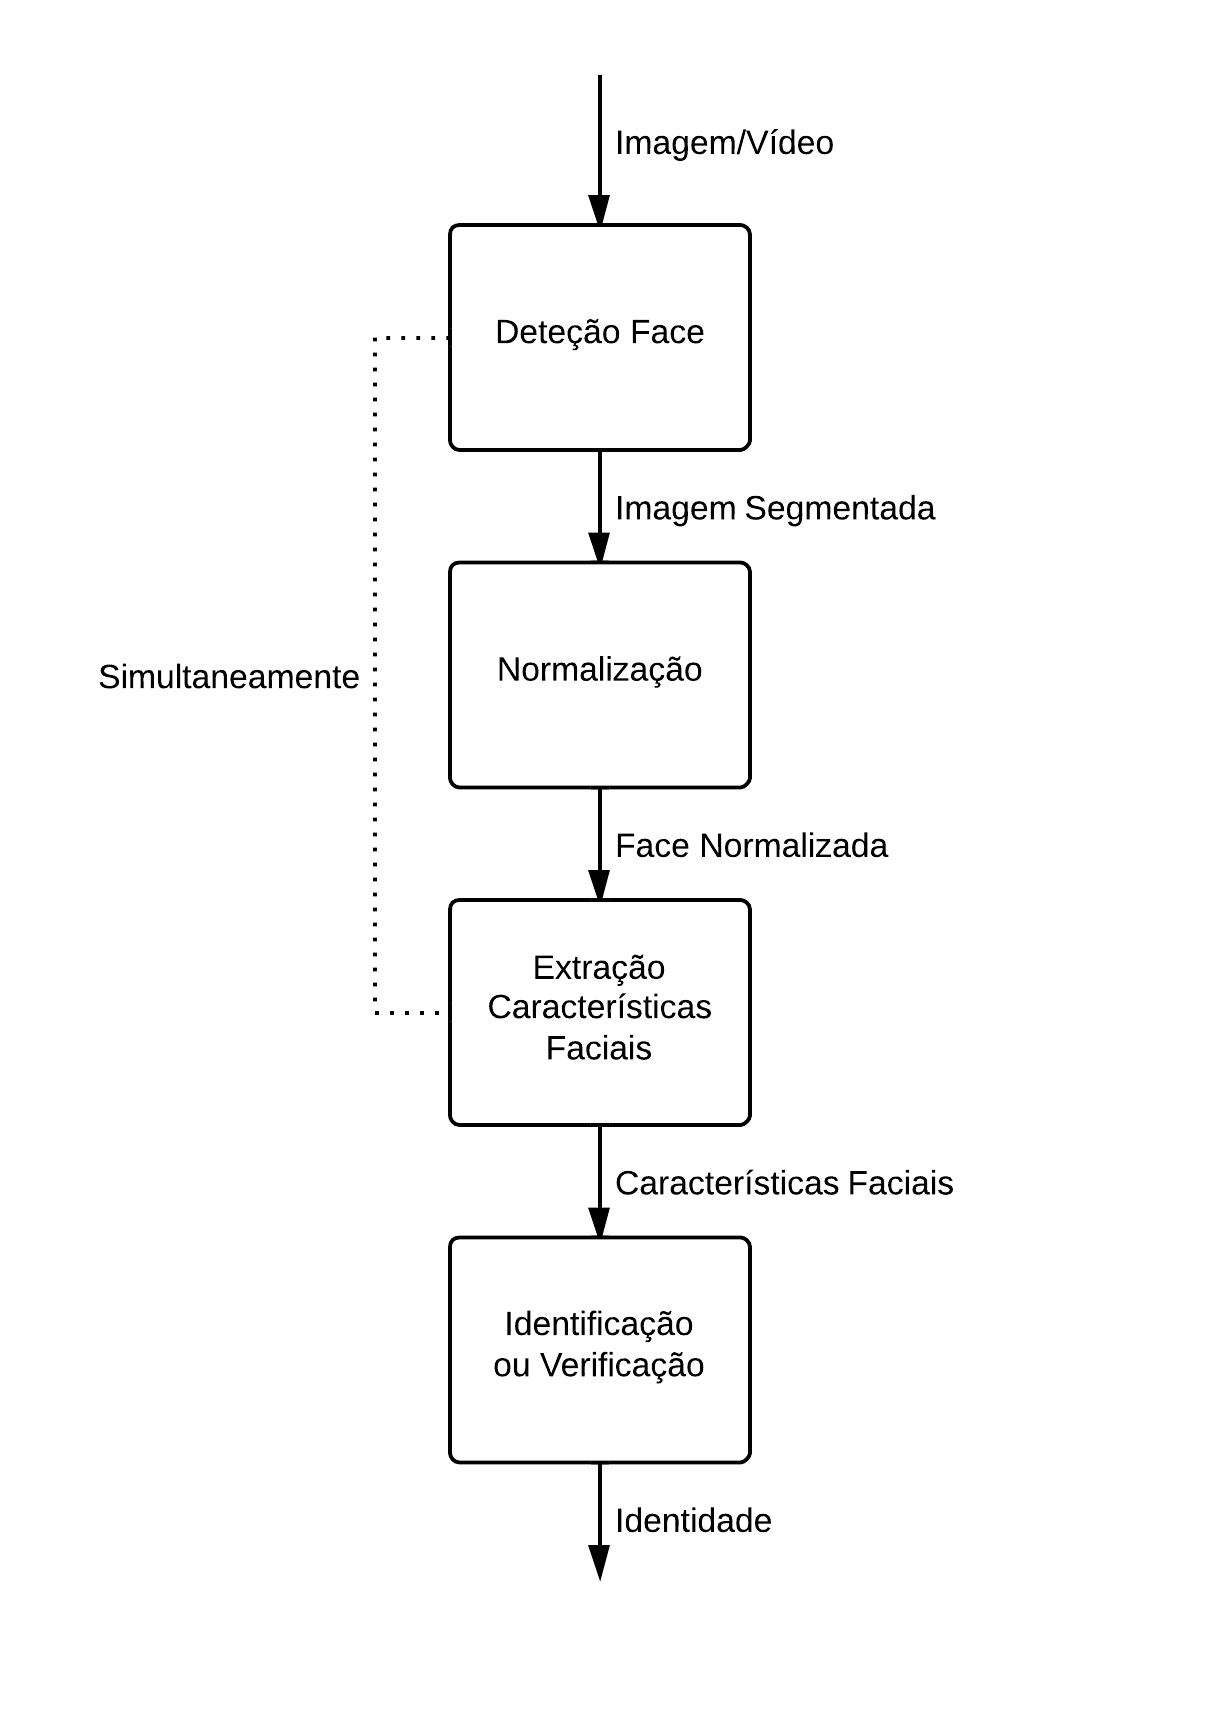
\includegraphics[width=0.5\textwidth]{SistemaGenericoRF}
    \caption{Sistema Genérico de Reconhecimento Facial}
    \label{fig:genericRF}
  \end{center}
\end{figure}

\subsection{Desafios} \label{desafios}
O reconhecimento facial automático em imagens é um problema complexo, sendo que existem um conjunto de desafios que se colocam na construção de um sistema de tipo. O primeiro passo em qualquer um desses sistemas, é a deteção de faces na imagem, a esse nível\textit{Yang et al.}, destacaram, no revisão ao estado da arte realizado em 2002,  os seguintes desafios \citep{Yang2002}:
\begin{itemize}
\item Pose e Orientação: A posição relativa da face à câmara pode sofrer uma grande variação dependendo do ambiente onde é capturada a imagem (variação no ângulo da face em relação à câmara vertical e horizontalmente, posição frontal, perfil). Ao variar a posição da face, alguns dos elementos que a permitem localizar e reconhecer podem ficar obstruídos. Avaliações efetuadas \citep{BlackburnDuaneM.;BoneMike;Phillips2001}, demonstram que este impacto é maior, quanto maior for o ângulo da pose em relação à posição frontal, sendo que uma variação até cerca de 25º não afeta significativamente os resultados do reconhecimento.
\item  Elementos Estruturais: a presença ou ausência de elementos estruturais, tais como barba ou óculos, assim como, a grande variação de forma e cor a que estes elementos podem apresentar afetam significativamente a forma como a face é percecionada pelo sistema.
\item Obstrução da face: as imagens captadas podem possuir objetos em frente à cara da pessoa a ser identificada, levando apenas a uma representação parcial da face na imagem.
\item Condições da imagem: aspetos como a resolução da imagem, o sensor utilizado para a captura e até mesmo eventuais defeitos associados à câmara utilizada podem potencialmente afetar o aspeto final da face na imagem.
\end{itemize}

Outro fator que afeta significativamente a perceção de uma face por um sistema de reconhecimento facial automático é a iluminação. Uma imagem pode ser capturada, com iluminação natural ou artificial. Para além disso, a iluminação pode estar sujeita a uma grande variação de tonalidades, intensidade e ângulo de incidência da luz.

Mesmo quando captadas pela mesma câmara, com as mesmas condições de iluminação e no mesmo local, podem existir variações significativas nas imagens captadas da face de uma pessoa devido às diferentes expressões faciais contidas nas imagens, fazendo com que este seja outro desafio a ultrapassar ao efetuar o reconhecimento facial automático.

O envelhecimento, ou eventuais alterações provocadas na face devido a fatores externos como por exemplo acidentes, exposição a condições extremas ou intervenção cirúrgica é outro dos fatores a ter em conta na identificação de uma pessoa.

Finalmente, existem ainda fatores como o elevado grau de semelhança entre pessoas com graus de parentesco próximos. Imagens capturadas de gémeos, ou até mesmo de pais e filhos, podem à primeira vista parecer imagens da mesma pessoa, tornando ainda mais difícil para um sistema automático efetuar a distinção dos indivíduos.

Assim sendo, para um reconhecimento fiável e eficaz é essencial que todas as etapas identificadas em \ref{sec:sub-problemas} sejam concluídas com sucesso. Sem uma correta deteção da presença de uma face na imagem, todos os passos subjacentes seriam impossíveis de ser realizados, por outro lado, o sucesso da extração das características faciais, encontram-se também dependente de uma normalização eficaz das imagens. No entanto, apesar desta dependência verificada entre as diversas etapas, cada uma delas representa problemas complexos, que devem a merecer a atenção e estudo de forma individual para que uma maior evolução das diversas técnicas envolvidas seja atingida \citep{Zhao2003}.


\section{Áreas de Aplicação}\label{sec:areasAplicacao}
O problema de reconhecimento facial automático tem merecido a atenção e estudo de inúmeros investigadores ao longo dos últimos 40 anos, motivados não só pelos desafios inerentes ao processo de reconhecimento facial, mas também pelas pela vasta gama aplicações onde a identificação de indivíduos é necessária \citep{Li2011}.

Adicionalmente, a evolução tecnológica da última década, permitiu a criação de sistemas computacionais mais poderosos, os quais tornaram possíveis desenvolvimentos na área que anteriormente seriam impensáveis gerando um ainda da maior interesse, tal como pode ser verificado pelo surgimento de uma vasta gama de aplicações comerciais e governamentais de reconhecimento facial, como é exemplo o sistema de fronteira automática dos aeroportos portugueses \citep{MinisteriodaAdministracaoInternaa}, assim como, pela recente aquisição de soluções de reconhecimento facial por parte de duas grandes empresas tecnológicas nomeadamente Google e Facebook.

De seguida encontram-se descritas, em cinco categorias, algumas das áreas de aplicação do reconhecimento facial automático, respetivamente ilustradas com exemplos de aplicação real. Esta categorização foi baseada no estudo efetuado em \cite{Li2011}, o qual é para nosso conhecimento o mais recente estudo efetuado às diversas áreas de aplicação do reconhecimento facial, assim como em estudos anteriores efetuados por \cite{Zhao2003}. Esta secção pretende apenas apresentar de uma forma sumária algumas das possíveis áreas de aplicação, e respetivas soluções, às quais o reconhecimento facial poderá ser aplicado, não pretendendo ser um estudo exaustivo de todas as soluções existentes.

\subsection{Controlo de Acesso e Segurança de Informação} \label{sec:controloAcesso}
A necessidade de sistemas de fácil utilização que assegurem a segurança da nossa informação digital, assim como da privacidade dos utilizadores, sem que para isso seja necessário a memorização e utilização de um sem número de palavras-chave e códigos de segurança é premente. Neste campo, o reconhecimento facial destaca-se ao permitir a criação de sistemas de autenticação não invasivos que requerem um nível de cooperação baixo por parte dos participantes, em contraste com os sistemas tradicionais como o uso de palavras-chave, ou mesmo de sistemas mais complexos como a análise de impressões digitais, retina ou íris. Por outro lado, este tipo de sistemas, permite ainda determinar a presença factual do utilizador que se pretende identificar, e não apenas determinar o conhecimento de um código de acesso à informação.

Atualmente, o uso de reconhecimento facial para o controlo de acesso a informação encontra-se já a ser utilizado em diversas aplicações comercias como são exemplos os sistemas de autenticação automática disponíveis numa grande variedade de computadores portáteis \ref{Asus, Hp, Topshiba}. De uma forma geral, nestes sistemas,o utilizador apenas necessita de se aproximar do computador para que o reconhecimento facial e consequente autenticação sejam efetuados. Desta forma o utilizador não necessita de efetuar qualquer intervenção para aceder aos seus dados ou de memorizar qualquer palavra-chave.

O uso de reconhecimento facial para garantir uma maior segurança de informação, ou efetuar um mais eficaz controlo do seu acesso, é geralmente aplicado em soluções com um número de utilizadores limitado e nas quais as imagens capturadas apresentam baixa variabilidade nas condições de iluminação e pose dos utilizadores. Desta forma, o nível de precisão do reconhecimento atingido nesta área é normalmente elevado, fazendo com que o nível de satisfação dos seus utilizadores seja também elevado \cite{Li2011}.

\subsection{Cartões Inteligentes e Identificação de Faces} \label{CartoesInteligentes}
Os documentos pessoais inteligentes registam uma presença cada vez mais ativa na sociedade atual, como é caso do cartão do cidadão português (CC), que à data de 5 de Novembro de 2012 já tinha sido adotado por mais de 7 milhões de portugueses \citep{Administrativa}, ou mesmo do passaporte eletrónico português (PEP), o qual recebeceu igualmente uma ampla aceitação desde a sua criação em 2006 \citep{MinisteriodaAdministracaoInterna}.

Tradicionalmente este tipo de documentos encontram-se dotados de capacidade de processamento e armazenamento próprios, podendo interagir com aplicações de terceiros como, por exemplo, sistemas de autenticação com recurso ao reconhecimento facial. O sistema designado de Reconhecimento Automático de Passageiros Identificados Documentalmente (RAPID)\citep{MinisteriodaAdministracaoInternaa}, desenvolvido pela empresa portuguesa Vision-Box \citep{Vision-Box} encontra-se desde 2007 em funcionamento nos vários aeroportos internacionais portugueses e tira partido das vantagens da associação da tecnologia de reconhecimento facial com documentos inteligentes. Em primeiro lugar, o sistema verifica se os dados armazenados no chip do passaporte são válidos, posteriormente, é efetuada uma comparação entre a fotografia armazenada no cartão e a imagem capturada do passageiro pelo dispositivo instalado na fronteira automática. Caso a identificação seja verificada, a porta que permite a passagem entre fronteiras é então automaticamente aberta. Todo o processo, encontra-se ainda a ser supervisionado por um operador numa cabine, o qual se encontra a supervisionar múltiplos dispositivos de identificação, sendo apenas necessária a sua intervenção quando não é efetuada uma identificação válida da pessoa.

O nível de precisão dos sistemas que tiram partido das sinergias entre cartões inteligentes e o reconhecimento facial apresenta uma correlação com o nível de atualização dos dados presentes nos documentos, sendo que  com um nível de atualização frequente é possível ser atingido um nível de satisfação elevado \cite{Li2011}, como se comprova pela bom funcionamento do sistema RAPID.
Contudo, esta é ainda uma área de investigação em aberto para que uma utilização destes sistemas de forma totalmente autónoma (sem que seja necessária a supervisão de um operador), em larga escala e, por exemplo, em ambientes não controlados seja possível.

\subsection{Entretenimento} \label{Entretenimento}
As tecnologias de reconhecimento facial apresentam uma forte potencialidade de aplicação nas área associadas ao entretenimento e à produção de conteúdos digitais, nomeadamente no que diz respeito à produção de jogo de computador e interação humano computador.

As consolas modernas estão dotadas de capacidade de processamento notáveis, para além disso, juntamente com estas consolas é cada vez mais comum o surgimento de dispositivos como o\textit{Kinect} da Microsoft que permitem novas formas de interação e a criação de novos tipos de jogos. Uma das novidades introduzidas pelo Kinect é a inclusão de diversos sensores e câmaras que permitem, entre outras coisas, efetuar um reconhecimento facial dos utilizadores. Desta forma, as equipas de desenvolvimento de jogos de computador, podem agora de uma forma mais fácil utilizar mecanismos de reconhecimento facial automático nos seus jogos de forma a criar jogos mais imersivos e personalizados. Este reconhecimento pode ainda ser aplicado ao nível da interação pessoa-computador  onde permite, a criação de sistemas com uma  uma maior facilidade de interação, uma vez que o próprio rosto poderá servir como um dispositivo de \textit{input} natural. 

À semelhança dos sistemas de controlo de acesso o reconhecimento facial automático na área do entretenimento é geralmente aplicado em soluções com um número de utilizadores limitado e onde o nível de precisão necessário não é muito alto fazendo assim com que a satisfação dos seus utilizadores seja, em geral, elevada.

\subsection{Gestão de Conteúdos Multimédia e Bases de Dados} \label{GestaoMultimedia}
A sociedade atual caracteriza-se pelo constante fluxo de informação a que os seus indivíduos se encontram expostos. A título de exemplo e de acordo com dados divulgados pela Intel\citep{IntelCorporation}, a cada minuto, são visualizados no Youtube 1,3 milhões de vídeos e carregadas para os seus servidores 30 novas horas de vídeo. Já o Flicker, no mesmo período de tempo, regista a visualização de 20 milhões de fotos e o carregamento de 3000 novas imagens para a sua plataforma. Segundo os mesmos dados, atualmente o número de dispositivos com ligação à Internet é equivalente ao da população mundial e é esperado que em 2015 seja o dobro dessa população.

Este crescimento verificado quer na quantidade de conteúdos produzidos, quer na diversidade de dispositivos que acedem a esses conteúdos, torna assim extremamente importante uma gestão e organização eficazes dos mesmos. Os métodos tradicionais de pesquisa e organização de conteúdos multimédia baseiam-se em anotações textuais associadas a estes conteúdos designadas de descritores. Com o uso de sistemas de reconhecimento facial é possível efetuar o reconhecimento das entidades presentes numa biblioteca multimédia mesmo que as suas fotografias não possuam qualquer anotação textual, uma vez que é feita uma análise da própria imagem e não apenas dos seus descritores, tornando-se assim um importante auxílio dos métodos tradicionais.

Atualmente existem no mercado diversas aplicações que permitem efetuar a organização de álbuns fotográficos  pessoais com recurso ao reconhecimento facial como por exemplo o Picasa da Google ou o iPhoto da Apple. Por outro lado, redes sociais como Google Plus e o Facebook, lançaram também recentemente serviços que permitem aos seus utilizadores a deteção e identificação automática de outros utilizadores presentes nas imagens carregadas para os seus servidores.

Apesar de a performance destes sistemas ter registado uma evolução notável nos últimos anos, a grande variabilidade associada às condições de captura de imagens e a grande quantidade de dados a ser processada faz com que exista ainda uma grande margem de evolução possível a este nível, sendo que a performance verificada ao nível do reconhecimento efetuado varia muito de acordo com a aplicação a analisar, assim como as características do conjunto de dados a organizar.

\subsection{Segurança e Aplicação da Lei} \label{sec:SegurancaAplicaçãoLei}
A preocupação com a segurança de instalações públicas e privadas, torna-se ainda mais premente em situações de grave crise económica como aquela que vivemos atualmente. Por outro lado, fatores como o controlo de emigração ilegal, preocupações relacionadas com a segurança de eventos com um grande impacto mediático ou mesmo o auxílio à investigação policial tornaram esta uma das áreas de aplicação que mais interesse despoletou por parte de sectores privados e governamentais desde o surgimento das primeiras tecnologias de reconhecimento facial.

Uma das aplicações mais comuns do reconhecimento facial em segurança é o reforço da vigilância da via pública. Desde 1998, diversas cidades implementaram sistemas de vigilância com recurso a reconhecimento facial, como são exemplos os sistemas instalados em \textit{Newham Borough of London}, \textit{Tampa (Florida)} e \textit{Virginia Beach (Virginia)} \citep{Li2011}.
Um outro exemplo, foi o sistema desenvolvido para os jogos olímpicos de 2008 em Pequim pela \textit{Chinese Academy Of Sciences} e que foi utilizado para validar as entradas nas cerimónias de abertura e encerramento dos jogos olímpicos \cite{ChineseAcademyOfSciences}.

A aplicação de sistemas de reconhecimento facial para a segurança e aplicação da lei tem atraído muita atenção por parte de sectores privados e governamentais, havendo o registo de alguns casos onde a sua aplicação se revelou um sucesso. Contudo, de uma forma geral estes sistemas debatem-se com um baixo nível de satisfação por parte dos seus utilizadores, isto porque, existe uma grande variabilidade nas condições de iluminação das imagens captadas, pose dos utilizadores, assim como, um número muito elevado de faces a analisar, resultando num número elevado de falsos positivos e consequentemente numa má performance dos sistemas \citep{Li2011}.

\section{Estratégias de Reconhecimento Facial}\label{sec:estratégias}
Após o trabalho inicial de Takeo Kanade em 1973 \citep{Kanade1973}, a área do reconhecimento facial automático passou um período de dormência até meados da década de 90, onde os trabalhos realizados recorrendo a métodos como \textit{Principal Component Analysis (PCA)}, \textit{Linear Discriminant analysis (LDA)} e \textit{Ellastic Grapth Matching (EGM)}, revitalizaram a área \citep{Chellappa2010}. Ao nível da PCA, o método
 \textit{Eingenfaces} desenvolvido por Turk e Pentland em 1991 \cite{Turk1991}, foi um marco fundamental no rejuvenescimento do reconhecimento facial automático. Este método tira partido da redundância natural existente entre as representações faciais de diversos indivíduos, para através de uma análise dos componentes principais das faces, desenvolvida anteriormente por Kirby e Sirovich  \cite{Kirby1990}, efetuar uma representação de baixo nível das faces existentes. Posteriormente, o método \textit{Fisherfaces} \cite{Belhumeur1997, Etemad1997, Zhao1998}, que tira partido da aplicação de LDA após uma análise inicial dos componentes principais da imagem, apresentou também resultados positivos em experiências em bases de dados com um número elevado de faces a analisar. Finalmente, ao nível de EGM, foi percursor o trabalho realizado por Wiskott \textit{et al.} \cite{wiskott1997face}. 
 
Desde então, diversos investigadores estenderam estes três tipos de algoritmos. Em 2003, Zhao \textit{et al.} \citep{Zhao2003} efetuaram um estudo aprofundado das técnicas desenvolvidas até então classificando-as em três categorias. Métodos holísticos, caso estes usem toda a região da face como fonte de comparação no reconhecimento, métodos baseados nas caraterísticas faciais, caso estes usem as características extraídas como informação essencial para a classificação da face e ainda como híbridos, caso seja utilizada uma mistura de ambos os métodos. Os resultados desta classificação podem ser visualizados na tabela \ref{tabelaZhao}.

\begin{center}
\begin{table}
	\caption{Categorização dos Métodos de Reconhecimento Facial em Imagens por Zhao \textit{et al.} \citep{Zhao2003}}
	% title of Table
	\centering
	% used for centering table
	\begin{tabular}{l p{8cm}}
	% centered columns (4 columns)
	\hline\hline
        Método                     & Trabalho Representativo\\
	% inserts table
	%heading
	\hline
		% inserts single horizontal line
Holistic methods	 \\	
$\quad$ \textit{Principal Component analysis (PCA)} \\
$\qquad$  Eigenfaces                 & Direct application of PCA [Craw and Cameron 1996; Kirby and Sirovich 1990; Turk and Pentland 1991] \\
$\qquad$        Probabilistic eigenfaces   & Two-class problem with prob. measure [Moghaddam and Pentland 1997] \\
$\qquad$        Fisherfaces/subspace LDA   & FLD on eigenspace [Belhumeur et al. 1997; Swets andWeng 1996b; Zhao et al. 1998] \\ 
$\qquad$        SVM                        & Two-class problem based on SVM [Phillips 1998] \\ 
$\qquad$        Evolution pursuit          & Enhanced GA learning [Liu andWechsler 2000a] \\ 
$\qquad$        Feature lines              & Point-to-line distance based [Li and Lu 1999] \\ 
$\qquad$        ICA                        & ICA-based feature analysis [Bartlett et al. 1998] \\ 
$\quad$ \textit{Other Representations} \\
$\qquad$        LDA/FLD                    & LDA/FLD on raw image [Etemad and Chellappa 1997] \\ 
$\qquad$        PDBNN                      & Probabilistic decision based NN [Lin et al. 1997] \\

Feature-based methods \\
$\qquad$        Pure geometry methods      & Earlier methods [Kanade 1973; Kelly 1970]; recent methods [Cox et al. 1996; Manjunath et al. 1992] \\ 
$\qquad$        Dynamic link architecture  & Graph matching methods [Okada et al. 1998;Wiskott et al. 1997] \\ 
$\qquad$        Hidden Markov model        & HMM methods [Nefian and Hayes 1998; Samaria 1994; Samaria and Young 1994] \\

Hybrid methods \\
$\qquad$        Convolution Neural Network & SOM learning based CNN methods [Lawrence et al. 1997] \\ 
$\qquad$        Modular eigenfaces         & Eigenfaces and eigenmodules [Pentland et al. 1994] \\ 
$\qquad$        Hybrid LFA                 & Local feature method [Penev and Atick 1996] \\ 
$\qquad$        Shape-normalized           & Flexible appearance models [Lanitis et al. 1995] \\ 
$\qquad$        Component-based            & Face region and components [Huang et al. 2003] \\
        \hline
    \end{tabular}
	\label{tabelaZhao}
\end{table}
\end{center}
 
 Tal como referido na secção \ref{desafios} deste relatório, o reconhecimento facial é uma tarefa complexa, composta por um conjunto de sub-problemas que enfrentam uma série de desafios para a sua conclusão. O primeiro desafio em qualquer sistema de reconhecimento facial é a deteção da face na imagem, a esse nível o trabalho realizado por Paul Viola e Michael Jones \citep{Viola2004} é considerado como um dos mais robustos métodos disponíveis na atualidade. Outras áreas onde a investigação atual se encontra focada têm a ver com a criação de métodos de reconhecimento facial robustos em relação à iluminação das imagens, assim como a pose dos indivíduos representados. \citep{Chellappa2010}.
 
 Ao nível da pose, o uso de  \textit{3D morphable face models} \cite{Blanz2003} tem revelado resultados positivos em posições não frontais. Estes algoritmos simulam o processo de formação de uma face em 3D, estimando a sua representação tridimensional a partir de imagens 2D fornecidas ao sistema com recurso a técnicas de computação gráfica. Esta estimativa é efetuada através do encaixe de um modelo 3D de faces na própria imagem fornecida, modelo esse apreendido através da digitalização 3D de um conjunto de rostos e respetiva textura. No entanto, em grande parte dos modelos desenvolvidos a seleção manual de um pequeno número de características faciais é requerida e o poder de computação necessário para a criação dos modelos é elevado. Extensões destes modelos foram também propostas para criar sistemas mais robustos em relação à variação na iluminação.  
 
 Outras abordagens que têm em vista a criação de sistemas de reconhecimento facial robustos em relação à iluminação centram os seus esforços na estimação do albedo para a normalização das imagens. O albedo representa a relação entre a quantidade de luz refletida por um ponto e quantidade de luz incidente, métodos recentes centram-se no desenvolvimento de filtros estocásticos não estacionários para a estimação de mapas de albedo das amostras faciais \cite{Biswas2009}. Estes mapas podem ainda ser combinados com os modelos 3D faciais desenvolvidos para uma representação facial mais completa. Apesar de os resultados obtidos por estes métodos serem promissores quando comparados com os métodos tradicionais como o \textit{Eigenfaces}, estes métodos ainda carecem de maior validação, uma vez que as suas avaliações foram feitas utilizando conjuntos de dados controlados e de reduzida dimensão \citep{Chellappa2010}.
 
O investimento realizado na investigação de metodologias de reconhecimento facial automático tem permitido progressos notáveis na área. Do mesmo modo, a investigação em áreas relacionadas como a deteção de faces nas imagens, o envelhecimento facial ou o reconhecimento de expressões faciais em imagens tem permitido evoluir ainda os resultados obtidos. Devido à complexidade envolvida no processo de reconhecimento facial automático a evolução na área encontra-se assim intrinsecamente ligada à evolução verificada nas múltiplas áreas envolvidas, sendo que a investigação independente de cada uma é crítica para uma resolução eficaz da grande variabilidade de desafios que o reconhecimento facial automático se propõe ultrapassar.

\subsection{Soluções Existentes}\label{sec:soluções}
A investigação desenvolvida nos vários centros de investigação na década de 90, levou à passagem das soluções de reconhecimento facial automático de meros protótipos de laboratório, para soluções comerciais de elevado valor acrescentado, dessas soluções resultaram três categorias comerciais de produtos na área do reconhecimento facial:
\begin{itemize}
\item Soluções Completas. Estas soluções caracterizam-se por oferecer toda a infraestrutura necessária para efetuar o reconhecimento facial, quer a nível de software, quer a nível de hardware.
\item Software. Soluções tradicionais de sistemas de reconhecimento facial, que consistem em software que permite efetuar o reconhecimento facial independentemente do hardware utilizado para a captura de informação.  Dentro destas soluções existe uma grande variedade nos produtos oferecidos, desde soluções baseadas na captura de imagens 2D estáticas, imagens 3D e vídeo. Para além disso, as soluções oferecidas encontram disponíveis para serem utilizadas em diversas plataformas, como por exemplo dispositivos móveis ou através da Internet.
\item SDK para reconhecimento facial. Permitem aos clientes, através de módulos independentes ou APIs, a criação de novas aplicações de reconhecimento facial.
\end{itemize}

Para além do reconhecimento facial automático, as soluções disponíveis possuem muitas vezes também associados outros métodos de biometria, como por exemplo reconhecimento de íris ou impressões digitais, assim como métodos mais tradicionais de autenticação como o uso de cartões de identificação ou passwords, de modo a aumentar a robustez e segurança dos sistemas.

Na tabela \ref{tab:solucoesExistente}, encontram-se listadas algumas das soluções comerciais atualmente existentes de reconhecimento facial, assim como alguns exemplos de aplicações onde estas foram utilizadas. Esta tabela não pretende representar um levantamento exaustivo das soluções existentes mas apenas ilustrar a vasta gama de produtos disponíveis.

Para além das soluções comerciais de reconhecimento facial ao longo dos últimos anos surgiram também algumas soluções gratuitas de reconhecimento facial. Deste tipo de soluções são exemplo o software Picasa da Google, ou software iPhoto da Apple que permitem aos seus utilizadores a organização de álbuns multimédia com recurso ao reconhecimento facial. Por outro lado, redes sociais como Google Plus e o Facebook, lançaram também recentemente serviços que permitem aos seus utilizadores a deteção e identificação automática de outros utilizadores presentes nas imagens carregadas para os seus servidores.


\section{Análises de Desempenho Efetuadas}\label{sec:performance}
A performance de um sistema de reconhecimento facial depende de uma grande variedade de fatores como a iluminação, posição da face na imagem, expressão facial e presença ou ausência de adereços (ex:óculos). Por outro lado, as condições de utilização do próprio sistema, tais como o número de utilizadores diferentes e a frequência de utilização, são também fatores a ter em conta ao avaliar a performance de um sistema. Uma avaliação apropriada dos sistemas de reconhecimento facial encontra-se então dependente da existência de uma base de dados de grandes dimensões e consequentemente um conjunto de casos de teste vasto, assim como, da existência de métodos apropriados para essa avaliação.

A criação do programa FERET em 1993, pelo NIST, permitiu assim colmatar uma lacuna existente na avaliação dos sistemas de reconhecimento facial existentes com a criação de uma base de dados de faces de grande dimensões assim como de um protocolo de avaliação dos respetivos sistemas de reconhecimento facial. Com base no protocolo desenvolvido foram levadas a cabo avaliações aos nos anos de 1994 e 1995. Um novo protocolo foi criado para a avaliação realizada em 1996. Posteriormente, o mesmo instituto realizou novas avaliações baseadas no protocolo FERET96 na edição de 2000 dos FRVT, a partir de 2002, um novo protocolo foi criado (protocolo FRVT 2002), com base no protocolo FERET96, mas com a particularidade de permitir a avaliação de sistemas de biometria em geral e não apenas sistemas de reconhecimento facial. Com base no novo protocolo criado foram então realizadas avaliações nos anos de 2002, 2006 e 2010. A decorrer encontram-se ainda as avaliações FRVT 2012. 

As avaliações levadas a cabo durante os programas FERET e FRVT constituem desta forma uma boa base para a análise da evolução dos sistemas de reconhecimento facial automático ao longo dos últimos 20 anos, tal como pode ser visto na figura \ref{fig:evolucaoAvaliacoes}. De seguida encontram-se descritas os principais objetivos e conclusões retiradas dos programas FERET e FRVT:

\subsection{FERET}
Para além dos objetivos anteriormente citados de criação de uma base de dados de grandes dimensões e de criação de um protocolo que permitisse uma avaliação concreta e de base científica dos algoritmos existentes, o programa FERET tinha ainda como propósitos avaliar o estado da arte e identificar futuras áreas de desenvolvimento do reconhecimento facial \cite{Phillips2000}. Tendo em conta estes objetivos, foi então avaliada a performance dos diferentes algoritmos em diferentes cenários, categorias de imagens e diferentes versões dos próprios algoritmos. A performance foi computada para situações de identificação e verificação de faces, estando os principais resultados da última avaliação, efetuada em 1996, descritos em Phillips \textit{et al.} \cite{Phillips2000}.

A primeira avaliação do programa FERET, em 1994, consistia num três de conjuntos de testes, cada um com uma galeria e conjunto de provas diferentes. O primeiro conjunto, consistia numa prova de reconhecimento de faces de uma galeria de 316 faces. O segundo, tinha com objetivo determinar a capacidade dos algoritmos de rejeitar faces não presentes na galeria, designadas de falso-alarme. O terceiro, tinha como objetivo analisar os efeitos da pose na performance dos algoritmos \citep{Phillips2000}.

Em 1995, teve lugar a segunda avaliação, com o objetivo de  avaliar os mesmo algoritmos em galerias de maior dimensão. A performance foi medida num único teste, com uma galeria de 817 indivíduos conhecidos, tendo sido dado um maior ênfase na avaliação de provas duplicadas. Um duplicado é uma imagem cuja imagem correspondente da galeria foi geralmente capturada em dias diferentes  \citep{Phillips2000}.

Na última edição, em 1996, e já com um protocolo atualizado, foram testados 12 algoritmos de reconhecimento facial, e estudada a sua performance em quatro situações diferentes, usando para isso uma galeria com um total de 1196 indivíduos. Na primeira situação, a galeria e as imagens de prova foram tiradas no mesmo dia e sobre as mesmas condições de iluminação. No segundo conjunto de provas, a galeria e as imagens de prova foram tiradas em dias diferentes. Para o terceiro teste, a galeria e as respetivas provas foram capturadas com pelo menos um ano de diferença. Finalmente, no quarto e último conjunto de testes, a galeria e as imagens de prova forma tiradas no mesmo dia, mas com diferentes condições de iluminação.

Várias conclusões foram retiradas das avaliações efetuadas. A primeira conclusão foi que, de facto, se verificava uma evolução nas técnicas de reconhecimento facial, uma vez que os resultados foram progressivamente melhores, mesmo quando comparadas versões diferentes do mesmo algoritmo. Essa conclusão é suportada pela análise dos resultados do caso geral de identificação, testado em todas as edições, onde as imagens da galeria e da prova foram capturadas no mesmo dia e com a mesma iluminação. Nesse teste em 1994, apenas 78\% indivíduos foram identificados com sucesso numa galeria de 317 indivíduos, ao passo que em 1995 foram identificados já 93 \% dos indivíduos numa galeria de 831 e nos testes da última edição (1996), 95\% dos indivíduos foi identificado numa galeria de 1196 indivíduos. De igual forma, foi também verificada evolução na deteção de duplicados, mantendo-se no entanto as percentagens de identificação de duplicados mais reduzidas quando comparadas com o caso geral de identificação devido à maior complexidade do problema.

Outra conclusão retirada foi que a performance se encontra dependente da galeria e conjunto de imagens de prova utilizadas, uma vez que foi verificado que mudando a galeria, mas mantendo o mesmo tipo de teste a ser efetuado a percentagem de indivíduos identificados varia significativamente. Para a galeria e conjunto de prova capturadas no mesmo dia a percentagem varia entre os 80\% e os 94\%, enquanto que para galeria e conjunto de prova, capturadas em dias diferentes essa percentagem varia entre os 24\% e os 69\% porcento. Para além disso, não se existiu qualquer algoritmo que se revelasse superior em todas as quatro situações de teste realizadas em 1996, variando as performances, conforme a situação de teste.

Finalmente, conforme a tarefa a efetuar, identificação ou verificação de faces, ficou também demonstrado que não havia uma técnica que se superiorizasse em ambas as situações, comprovando que o reconhecimento facial é uma tarefa complexa que necessita de um estudo e investigação concretos tendo em conta a área de aplicação em vista.

\subsection{FRVT}
Durante a década de 90 registou-se um progresso assinalável nas diversas técnicas de reconhecimento facial, tendo para isso sido muito importante o papel desempenhado por iniciativas como o FERET. No final da década de 90, assistiu-se então a uma passagem dos sistemas de reconhecimento facial existentes de meros protótipos universitários, para aplicações comerciais de reconhecimento facial automático, tal como pode ser comprovado  pela participação de 5 soluções comerciais na primeira edição dos \textit{Facial Recognition Vendor Test}, no ano 2000. Esta avaliação, tinham como objetivo maioritário efetuar uma avaliação técnica das capacidades dos sistemas comerciais de reconhecimento facial disponíveis, de forma a compreender os pontos fortes e fracos de cada sistema, obtendo também uma análise do estado da arte do reconhecimento facial à data \cite{BlackburnDuaneM.;BoneMike;Phillips2001}. Estas avaliações foram ainda repetidas em 2002, 2006, 2010 e ainda em 2012.

A primeira edição dos FRVT, em 2000, utilizou o mesmo protocolo de avaliação da avaliação última avaliação FERET em 1996, no entanto, os testes efetuados eram significativamente mais exigentes do que a avaliação anterior, sendo utilizada também uma muito maior variedade de imagens. Os resultados da avaliação efetuada foram ser reportados para as seguintes oito categorias: compressão, distância, expressão,  media, iluminação, pose, resolução e variação temporal. Ao nível das conclusões retiradas, podem ser destacados os seguintes tópicos \cite{BlackburnDuaneM.;BoneMike;Phillips2001, Chellappa2010, Li2011}:
\begin{itemize}
\item Compressão de imagens, utilizado JPEG, até 40:1 não reduziu a taxa de reconhecimento;
\item Pose não afeta o reconhecimento de forma significativa até $\pm$ 25º, mas afeta significativamente quando são atingidos os $\pm$ 40º;
\item De forma equivalente ao registado no programa FERET, o uso de diferentes iluminações interiores não afeta significativamente os resultados obtidos, no entanto esses resultados são afetados caso haja uma mudança entre zonas interiores e exteriores;
\item Registou-se uma melhoria significativa dos resultados obtidos em imagens tiradas com mais de 18 meses de distância, quando comparado com os resultados obtidos no FERET. (Aumento de 5\% a 12\% de faces identificadas conforme o conjunto de dados avaliado).
\end{itemize}

A segunda edição dos FRVT teve lugar em 2002, contou com a participação de soluções de reconhecimento facial de 10 empresas distintas. Esta edição consistiu em duas provas fundamentais, os \textit{High Computational Intesity test (HCInt)} e os \textit{Medium Computational Intensity test (MCInt)}. Os HCInt tinham como objetivo medir a performance dos sistemas existentes em 121 589 imagens frontais de 37 435 pessoas, representando um desafio computacional de elevado grau de exigência, como comprovado pelas 242 horas de computação necessárias para efetuar os testes. Os \textit{Medium Computational Intensity test (MCInt)}, assemelhavam-se às medições efectuadas em avaliações anteriores, como o FERET e o FRVT 2000, tendo como objetivo medir a performance dos sistemas em imagens de diferentes categorias, nomeadamente não frontais, capturas no interior e exterior, entre outros. As conclusões retiradas desta avaliação foram as seguintes \cite{Chellappa2010, Li2011}:
\begin{itemize}
\item Melhores sistemas são insensíveis a variações de luz interior;
\item Reconhecimento facial em imagens exteriores é ainda um desafio por resolver;
\item Utilização de \textit{3D morphable models} melhora a performance em situações não frontais;
\item Características como sexo e idade podem afetar significativamente a performance, sendo que se registou maior facilidade em distinguir homens e pessoas com idade superior.
\item O tempo de captura entre provas afeta significativamente a performance, registando-se uma diminuição linear da performance com o aumento do tempo.
\end{itemize}

As últimas edições dos FRVT para as quais foram divulgados resultados foram as edições de 2006 \cite{Phillips2007} e a de 2010. Na edição de 2010 a competição não assumiu o nome de FRVT 2010, mas sim de \textit{Multiple Biometric Evaluation (MBE)} 2010-\textit{still image track}, uma vez que além de avaliados sistemas de reconhecimento facial automático foram também avaliados sistemas de biometria com base na análise da íris. \cite{Grother2010}. Foi também realizada uma edição dos FRTV em 2012, mas a avaliação dos sistemas ainda se encontra a decorrer, não havendo por isso resultados divulgados.

\begin{figure}[t]
  \begin{center}
    \leavevmode
    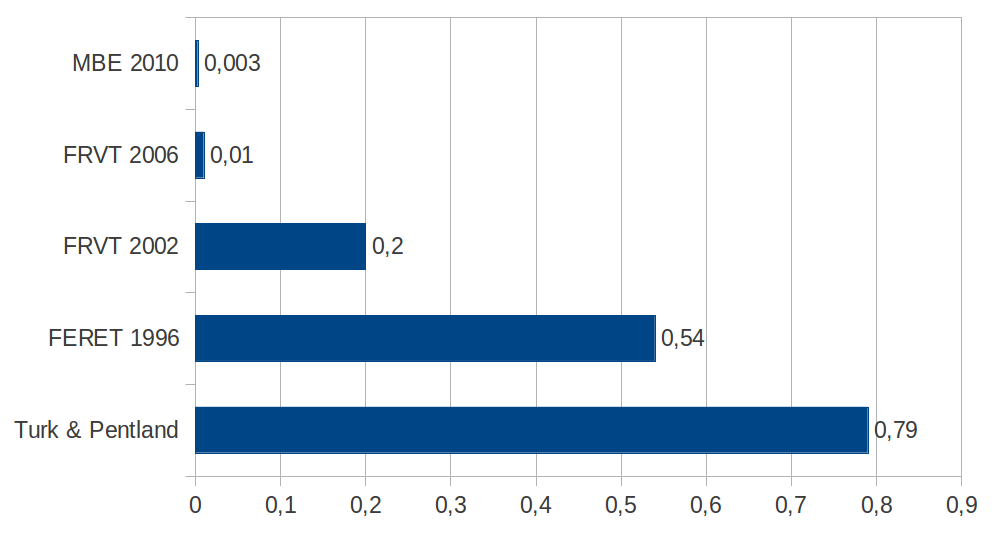
\includegraphics[width=0.9\textwidth]{EvolucaoAvaliacoes}
    \caption{A redução da taxa de erro para os algoritmos estados da arte tal como documentado nas avaliações FERET, FRVT 2002, FRVT 2006 e MBE 2010 \cite{Phillips2007, Grother2010}}	
    \label{fig:evolucaoAvaliacoes}
  \end{center}
\end{figure}

Em 2006, foi analisada a performance de sistemas de reconhecimento facial, de 22 organizações e de 10 países diferentes, baseados em representações 3D e em imagens estáticas de faces. As avaliações consistiam em três testes distintos: comparação de imagens capturadas com luz interior; comparação de digitalizações de faces 3D com base na forma e textura; comparação de imagens capturadas em estúdio com imagens capturadas em corredores e átrios. Em 2010, para além do conjunto de dados analisados em 2006 e 2002, de modo a averiguar a evolução comparativa dos algoritmos, foi também analisado um segundo conjunto de imagens recolhidas por várias agências de segurança e compiladas pelo \textit{Federal Bureau of Investigation (FBI)}. Este segundo conjunto de dados possuía mais de 1 milhão de faces fazendo da avaliação de 2010 a avaliação em maior escala feita aos sistemas de reconhecimento facial à data. Das provas de 2006 e 2010, as principais conclusões obtidas foram as seguintes \cite{Phillips2007, Grother2010, Chellappa2010, Li2011}:
\begin{itemize}
\item Desde 1993 foram atingidas melhorias de 2 ordens de magnitude;
\item Os resultados de 2010 e 2002 mostram uma melhoria de 1 ordem de magnitude nos sistemas de reconhecimento facial (Para um \textit{false accept rate (FAR)} de 0.001, foi registado em 2002 um \textit{false reject rate (FRR)} de 0.2, enquanto que em 2010 FRR=0.038);
\item Em condições de captura de informação controlada, a performance medida de sistemas de reconhecimento facial e sistemas baseados na análise da íris foi equivalente;
\item A performance de sistemas baseados em imagens estáticas e sistemas baseados em representações 3D da face foi equivalente;
\item Iluminação e resolução das imagens representam um papel fundamental no reconhecimento facial;
\end{itemize}
\chapter{Abstração de Imagens} \label{chap:abstracao} - TO-DO
A abstração de imagens permite uma simplificação do conteúdo visual ao retirar informação redundante e dar destaque apenas à informação essencial representada. Desta forma, os artistas têm a capacidade  de guiar a atenção de quem visualiza a imagem para conteúdos específicos, influenciando assim a perceção da mesma e tornado a comunicação mais eficaz.

Este filtros permitem uma simplificação do conteúdo visual ao retirar informação redundante e destacando a apenas a informação essencial. Estes filtros são tradicionalmente utilizados por artistas para comunicar de uma forma mais eficaz a informação pretendida ao retirar a informação desnecessária de imagens foto-realistas \citep{Kyprianidis2009}.


\section{Resumo ou Conclusões}

\chapter{Sistema de Reconhecimento Facial Visage} \label{chap:visage}

Intro ...


\section{Filtros de Abstração de Imagens no Reconhecimento Facial}
O reconhecimento facial em imagens sofreu uma evolução notável nos últimos 20 anos, tal como documentado no Capítulo \ref{chap:reco}. 

Em cenários cooperativos com condições de captura de imagens controladas, nomeadamente ao nível da pose, iluminação e expressões faciais, considera-se mesmo que o problema de verificação 1:1 se encontra praticamente resolvido, uma vez que as taxas de reconhecimento atingidas são satisfatórias para a grande maioria das aplicações \cite{Li2011}. Existem também várias aplicações em situações reais com um bom nível de satisfação por parte dos seus utilizadores, como é o caso do sistema de fronteira automático dos aeroportos portugueses (ver \ref{CartoesInteligentes}), ou o controlo de entradas nas cerimónias inaugurais dos jogos olímpicos de Pequim (ver \ref{sec:SegurancaAplicaçãoLei}). Em condições específicas e favoráveis, é então possível considerar que os sistemas de reconhecimento facial automático atuais conseguem mesmo ultrapassar a capacidade de reconhecimento humana, uma vez que conseguem identificar com precisão um maior número de faces do que aquelas que um humano consegue.

Contudo, o problema de reconhecimento facial automático ainda se encontra longe de ser um problema totalmente resolvido. Em cenários onde é registada uma grande variação ao nível da pose, iluminação ou outros fatores identificados na Secção \ref{desafios}, a identificação das entidades capturadas é ainda uma área de investigação em aberto \cite{Li2011}. Para além disso, o desempenho e satisfação obtida por parte dos utilizadores dos sistemas atuais demonstra uma grande variação tendo em conta as situações onde estes sistemas são utilizados. 

Por outro lado, a crescente ubiquidade tecnológica e poder computacional presente nos diversos dispositivos utilizados no nosso dia a dia aumenta o leque de aplicações possíveis do reconhecimento facial automático, apresentando novos desafios às soluções atualmente existentes (ver \ref{sec:areasAplicacao}).

Considerando todos os fatores mencionados anteriormente , o elevado custo soluções comerciais existentes e ainda a falta soluções abertas, torna-se pertinente a realização de investigação na área do reconhecimento facial em imagens. 

Ao nível da abstração de imagens, estudos efetuados demonstraram que aplicação de filtros de abstração de imagens na recuperação de informação multimédia, nomeadamente no âmbito da da ilustração automática de texto, tem a potencialidade de melhorar a informação retornada, assim como reduzir significativamente as necessidades de processamento e armazenamento das imagens \cite{Coelho:2012:IAC:2260641.2260676}. 

Tendo em conta a importância e a necessidade de investigação na área do reconhecimento facial automático, e uma vez que não existem estudos relativos à utilização de filtros de abstração no processo de reconhecimento facial, torna-se pertinente o estudo do seu impacto. A hipótese levantada no âmbito desta dissertação é então que o uso da abstração em imagens que vão ser ser alvo de reconhecimento facial pode melhorar o processo de reconhecimento facial automático em imagens.

\section{Visage - Visão geral} \label{sec:visage}
A criação do sistema Visage teve como principal objetivo o desenvolvimento de um sistema de reconhecimento facial automático que permita analisar qual o impacto da abstração de imagens e outras tarefas de pré-processamento no processo de reconhecimento facial automático. 

O sistema é composto por um conjunto de aplicações do tipo seguindo um paradigma de caixa preta. Neste paradigma, para um conjunto de dados de entrada é produzido um resultado específico. Com o sistema desenvolvido pretende-se ainda a criação de uma base sólida que permita o desenvolvimento de futuras aplicações que tirem partido do reconhecimento facial automático no seu funcionamento, como por exemplo, aplicações na área de \textit{image retrieval}.

De uma forma genérica, o funcionamento do sistema Visage pode ser agrupado nas seguintes fases fundamentais:
\begin{description}
\item[Pré-processamento] Corresponde à primeira etapa executada, na qual é fornecida uma galeria de imagens a pré-processar, as quais irão ser posteriormente utilizadas na fases de treino e identificação. O pré-processamento engloba tarefas como deteção das faces na imagem, normalização do contraste e iluminação, aplicação de filtros de abstração ou alinhamento das imagens.
\item[Treino] Nesta fase são fornecidas um conjunto de imagens anotadas ao sistema e pretende-se que este crie uma base de conhecimento que permita de futuro proceder à identificação de novas imagens de acordo com a informação treinada.
\item[Identificação] Corresponde à utilização do sistema como o intuito de identificar novas imagens não anotadas. Para uma dada imagem fornecida ao sistema, este deve devolver no nome da pessoa que se encontra na imagem tendo em conta a informação obtida na fase de treino. Nesta fase é também possível obter uma lista de entidades, ordenada de forma crescente pela similaridade em relação à pessoa representada na imagem.
\end{description}

Uma vez que foco desta dissertação não é o desenvolvimento de algoritmos de reconhecimento facial, mas sim a análise do impacto da manipulação efetuada sobre as imagens a reconhecer, foram utilizadas bibliotecas de código aberto que fornecem a implementação de algoritmos bem estabelecidos para o reconhecimento facial automático e facilitam a manipulação efetuada sobre as imagens. Por outro lado, a utilização destas bibliotecas permite também a contribuição para uma área onde as soluções abertas existentes são ainda poucas.

Para a manipulação das imagens e implementação do sistema de reconhecimento facial foi utilizada a biblioteca \textit{Open Source Computer Vision Library} (\textit{OpenCV}), uma biblioteca de código aberto nas áreas de visão por computador e \textit{machine learning}, onde se encontram implementados mais de 2500 algoritmos relacionados com as áreas de computação gráfica e visão por computador. Esta biblioteca possui uma comunidade de mais do que 47 mil utilizadores, já registou mais de 5 milhões de downloads e é utilizada globalmente por empresas como a Google, Yahoo, Microsoft, Intel, IBM, Sony, Honda, Toyota \cite{Team}. Ao nível do reconhecimento facial, esta biblioteca disponibiliza um módulo denominado \textit{Face Recognizer}, onde se encontram implementados os algoritmos \textit{Eigenfaces}, \textit{Fisherfaces} e \textit{Local Binary Patterns Histograms}. Tendo em conta a ampla utilização da biblioteca OpenCV e a sua constante atualização pela comunidade, assim como as facilidades providenciadas pelo módulo de reconhecimento facial, esta foi considerada a biblioteca a utilizar como base de implementação do sistema de reconhecimento facial a criar.

Ao nível dos filtros de abstração foram utilizados os filtros gaussiano e bilateral, implementados na biblioteca \textit{OpenCV}, e ainda o filtro anisotrópico kuwahara, recorrendo para a sua utilização à implementação efetuada por Kyprianidis \textit{et al.} \cite{Kyprianidis2009} do mesmo filtro.

Finalmente, ao nível das galerias de imagens, foi utilizada a coleção \textit{Labeled Faces in the Wild} descrita na secção seguinte.


\section{Coleção de dados - \textit{Labeled Faces in the Wild}} \label{sec:lfw}

A evolução do reconhecimento facial automático em imagens tem beneficiado do aumento dos recursos disponíveis para o seu estudo, nomeadamente através da criação de novas e mais completas coleções de dados \cite{Huang2007}. A grande maioria destas coleções caracteriza-se por ter condições de captura controladas, com o intuito de efetuar o estudo de fatores específicos que afetam a qualidade do reconhecimento. A análise do problema de reconhecimento facial automático de um ponto de vista geral implica a escolha de uma biblioteca apropriada e que represente a grande variabilidade associada aos diferentes desafios que afetam o reconhecimento facial em imagens.

Para o desenvolvimento do sistema de reconhecimento facial Visage e posterior análise dos resultados foi escolhida a biblioteca de imagens \textit{Labeled Faces in the Wild}.

A biblioteca \textit{Labeled Faces in the Wild (LFW)} é uma base de dados fotográfica desenhada especificamente para o estudo do problema de reconhecimento facial, particularmente em situações onde as condições de captura das imagens não possuem restrições. Nesse sentido, as imagens que constituem a galeria caracterizam-se por possuir uma grande variabilidade, nomeadamente ao nível da pose, expressão, iluminação, etnia, idade, género, vestuário e qualidade da câmara com a qual foi efetuada a captura \cite{Huang2007}.

Nesta coleção encontram-se representados 5749 indivíduos, ilustrados por 13233 imagens. O número de imagens por pessoa apresenta no entanto uma grande variação, desde um mínimo de 1 imagem por pessoa para 4069 indivíduos, até um máximo de 530 imagens que representam o antigo presidente dos Estados Unidos da América George W. Bush. O gráfico na Figura \ref{fig:distribuicaoLFW} ilustra a grande variação da distribuição do número de imagens por pessoa. No eixo vertical encontram-se representadas o número de pessoas em escala logarítmica e no eixo horizontal o número de imagens correspondente.

\begin{figure}[ht]
  \begin{center}
    \leavevmode
    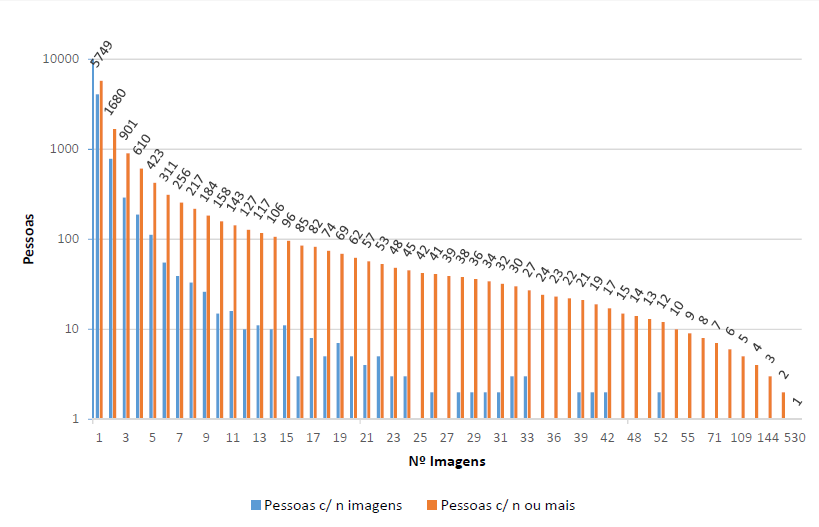
\includegraphics[width=1\textwidth]{Distribuicao}
    \caption{Distribuição do número de imagens por pessoa na biblioteca LFW.}
    \label{fig:distribuicaoLFW}
  \end{center}
\end{figure}

Devido à inexistência de restrições na captura de imagens, cada fotografia pode possuir mais do que uma face representada, sendo que a face que contém o píxel central deve ser considerada como a entidade representada na imagem. As imagens desta coleção são maioritariamente a cores, com diferentes graus de saturação, existindo também um número reduzido de imagens a preto e branco. A cada imagem encontra-se também associada uma anotação textual, relativa ao nome da pessoa representada. A Tabela \ref{tab:lfw} sintetiza algumas das características mais significativas da biblioteca. Nesta tabela são reportadas as caraterísticas da biblioteca no formato de imagens PNG uma vez que este foi o formato utilizado para avaliação do impacto dos filtros de abstração no processo de reconhecimento.

\begin{center}
\begin{table}
	\caption{Caracterização da Biblioteca LFW}
	\begin{center}
    \begin{tabular}{ll}
    \hline
    Característica                            & Valor            \\ \hline
    Imagens                                   & 13233 imagens    \\
    Pessoas representadas                     & 5749 pessoas     \\
    Tamanho total                             & 1.18 GB          \\
    Formato                                   & PNG              \\
    Tamanho de cada imagem: min / médio / max & 46.49 KB/ 93.72 KB/ 147.89 KB\\
    Dimensões imagem                          & 250$\times$250 píxeis \\
    \hline
    \end{tabular}
	\label{tab:lfw}
	\end{center}
\end{table}
\end{center}

Para além da coleção LFW original, encontram-se também disponíveis para fins de investigação duas outras coleções derivadas da coleção original, LFW funneled e LFW-a, onde as imagens originais foram sujeitas a um pré-processamento com vista a efetuar o alinhamento da posição da face na imagem, cada uma correspondendo a uma técnica diferente de alinhamento da imagem. Um exemplo de uma variante da mesma foto nas diferentes bibliotecas pode ser visto na Figura \ref{fig:lfwversoes}.

\begin{figure}[h]
        \centering
        \begin{subfigure}[b]{0.25\textwidth}
                \centering
                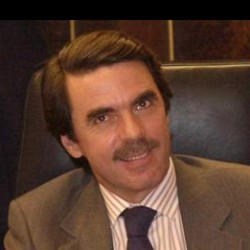
\includegraphics[width=\textwidth]{lfw_versoes/lfw}
                \caption{LFW}
                \label{fig:lfw_original}
        \end{subfigure}%
        ~ 
        \begin{subfigure}[b]{0.25\textwidth}
                \centering
                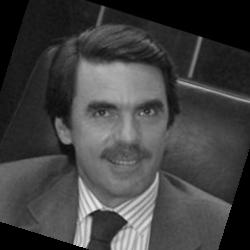
\includegraphics[width=\textwidth]{lfw_versoes/lfw-a}
                \caption{LFW-a}
                \label{fig:lfw_a}
        \end{subfigure}
        ~ 
        \begin{subfigure}[b]{0.25\textwidth}
                \centering
                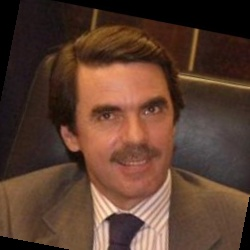
\includegraphics[width=\textwidth]{lfw_versoes/lfw-funneled}
                \caption{LFW funneled}
                \label{fig:lfw_funneled}
        \end{subfigure}
        \caption{Diferentes versões da biblioteca LFW}\label{fig:lfwversoes}
\end{figure}

A coleção LFW é particularmente interessante para o estudo do desempenho do sistema desenvolvido e consequentemente do impacto do uso da abstração de imagens no reconhecimento facial, uma vez que a variabilidade presente nas suas imagens, devido ao facto de estas não terem sido capturadas com o intuito específico da análise deste problema, representa uma amostra aproximada das variações encontradas no dia-a-dia de uma pessoa \cite{Huang2007}. Por outro lado, e uma vez que não pretendemos analisar a tarefa de alinhamento da face, a existência de versões já alinhadas da coleção permitiu retirar um fator importante de variação dos resultados obtidos. Assim sendo, optamos pela utilização da versão alinhada LFW-a para fins de avaliação do desempenho do sistema de reconhecimento facial criado e do impacto do uso de filtros de abstração no processo de reconhecimento.

\section{Arquitetura}
O sistema de reconhecimento facial criado é constituído pelos seguintes 6 módulos:

\begin{description}
\item[\textit{Person}] Módulo responsável por efetuar o encapsulamento da informação relativa a uma pessoa, nomeadamente o seu nome, código de identificação e imagens a esta associada. De modo a facilitar a avaliação do sistema criado é ainda possível armazenar de forma diferenciada imagens de treino e teste de cada pessoa.
\item[\textit{Library}]Módulo responsável por encapsular a informação de uma galeria de imagens utilizada para treinar o sistema, nomeadamente o seu diretório, as pessoas representadas nessa biblioteca (agrupadas num \textit{array} de objetos do tipo \textit{Person}) e alguns dados estatísticos como o número mínimo e máximo de imagens existentes por pessoa e o número total de imagens da galeria. Apesar de poder ser utilizado com diferentes funcionalidades este módulo foi desenvolvido com o intuito de facilitar a avaliação do sistema Visage com diferentes galerias de imagens, pelo que na criação de uma \textit{Library} é possível definir qual a percentagem das imagens, de cada pessoa, que devem ser utilizadas como conjunto de teste e conjunto de treino do sistema (Ver Capítulo \ref{chap:resultados} para mais detalhes).
\item[\textit{FaceDetector}] A par do módulo \textit{FaceModel} é um dos componentes principais do sistema, sendo responsável por efetuar um conjunto de tarefas de pré-processamento sobre as imagens utilizadas. Este módulo encontra-se descrito detalhadamente na Secção \ref{sec:facedetector}.
\item[\textit{FaceModel}] 
O módulo \textit{FaceModel} constitui uma camada de nível superior implementada para encapsular a comunicação com módulo de reconhecimento facial disponível na biblioteca \textit{OpenCV}, designado \textit{FaceRecognizer}, assim como estender algumas das funcionalidades do mesmo. Este módulo encontra-se descrito com maior detalhe na Secção \ref{sec:facemodel}.
\item[\textit{Evaluator}] Módulo responsável por agrupar os métodos e objetos utilizados para efetuar a avaliação do sistema.
\item[\textit{Utils}] Engloba algumas funções úteis utilizadas para o desenvolvimento e avaliação do sistema Visage que não se enquadram no âmbito dos restantes módulos.
\end{description}

\section{Módulo \textit{FaceDetector}} \label{sec:facedetector}
O módulo \textit{FaceDetector} é um dos componentes principais do sistema de reconhecimento facial criado, sendo responsável por efetuar um conjunto de tarefas de pré-processamento sobre as imagens fornecidas ao sistema.

\begin{figure}[t]
  \begin{center}
    \leavevmode
    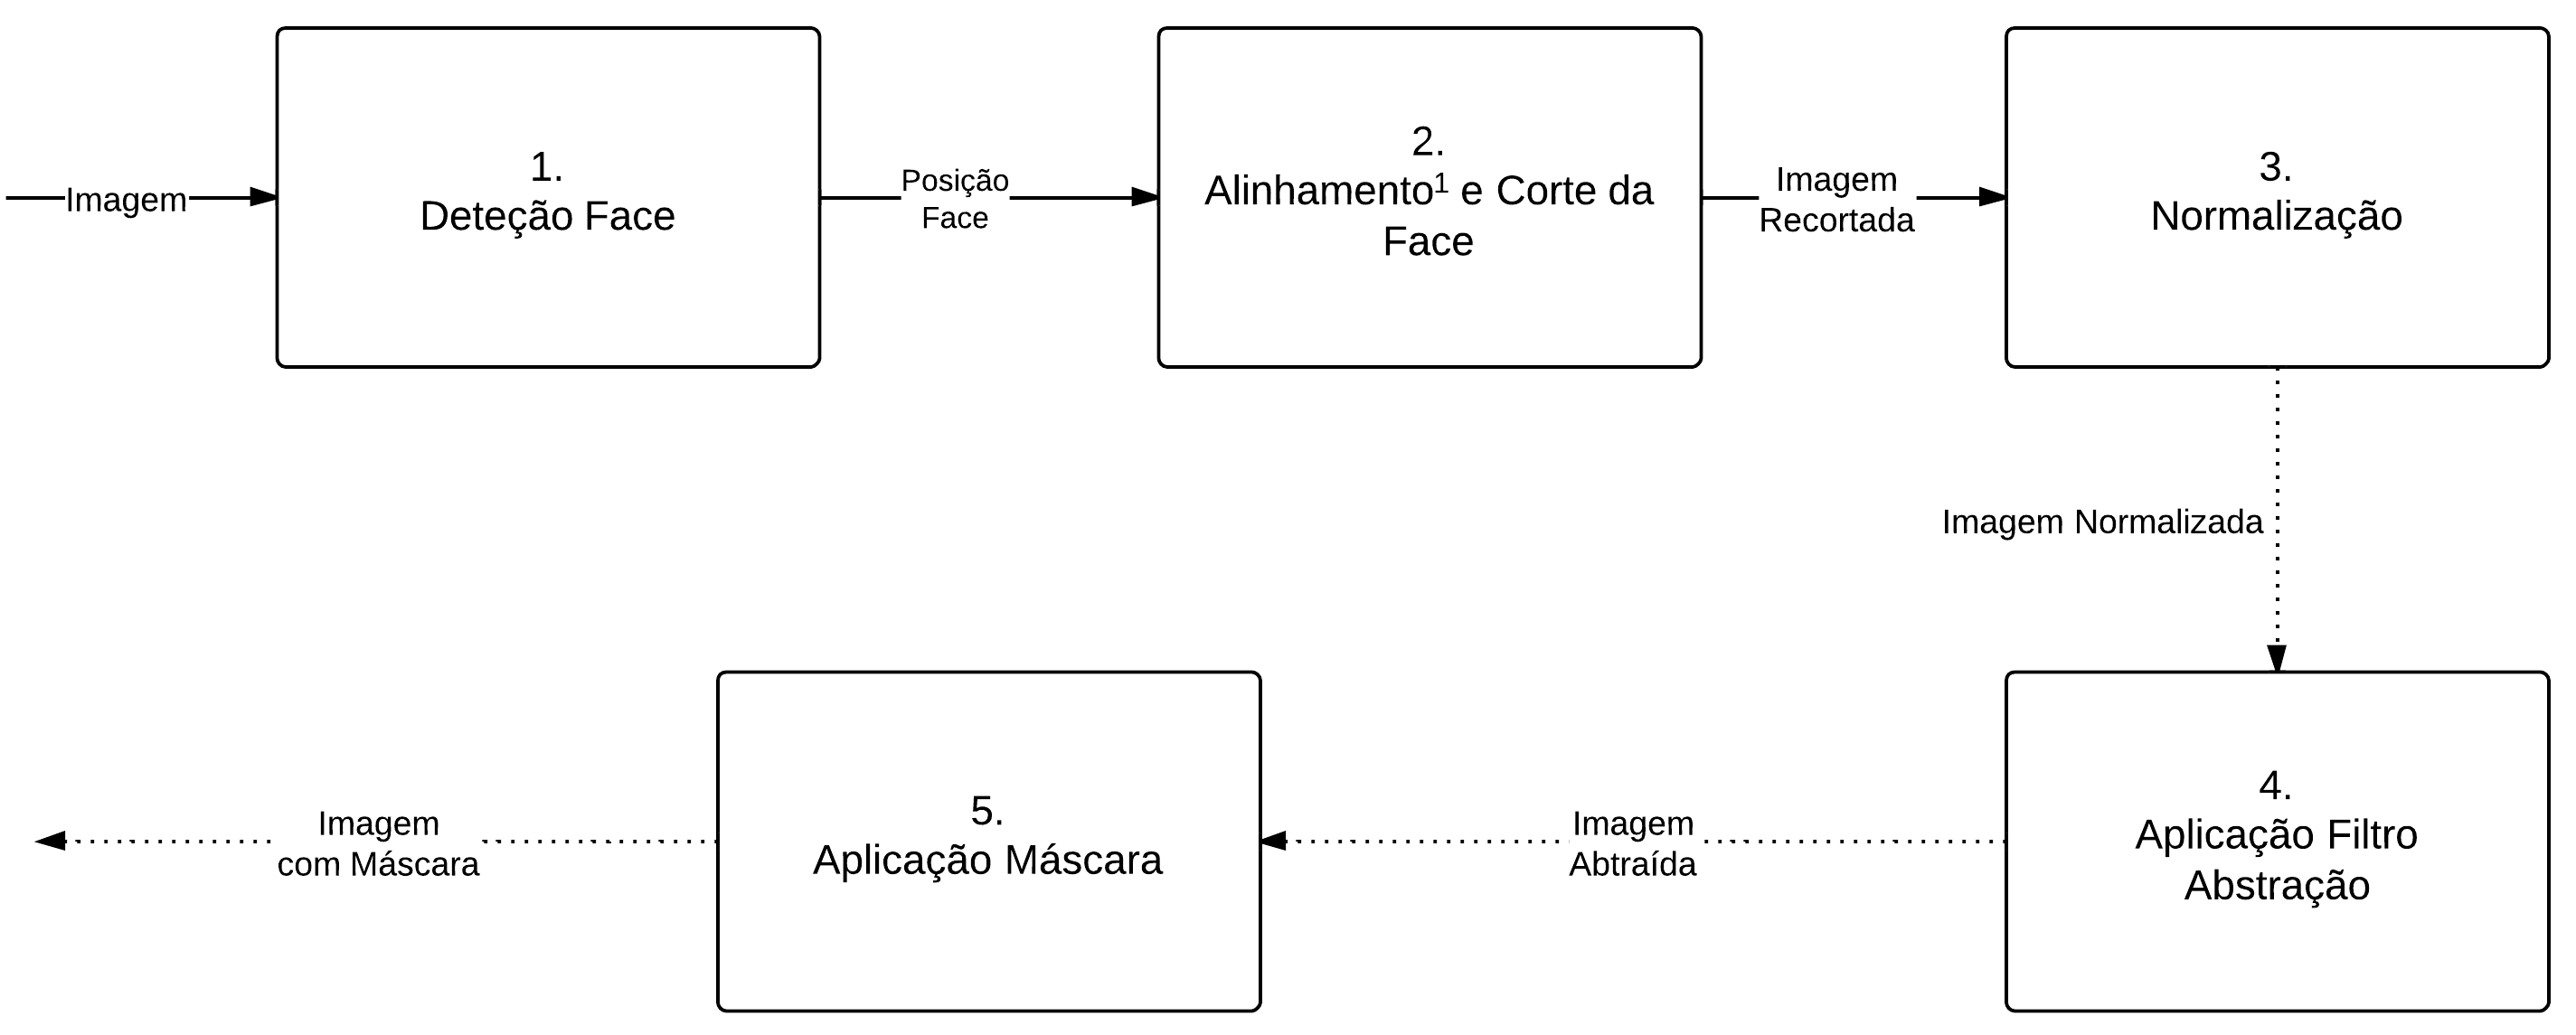
\includegraphics[width=1\textwidth]{PreProcessamentoVisage}
    \caption{Tarefas de pré-processamento disponíveis no sistema Visage.}
    \label{fig:preprocessamento}
  \end{center}
\end{figure}


Na Figura \ref{fig:preprocessamento} encontram-se representadas as tarefas de pré-processamento disponíveis no sistema de reconhecimento facial Visage, assim como a ordem pela qual as mesmas são aplicadas. As etapas de normalização, aplicação do filtro de abstração e aplicação da máscara constituem tarefas de pré-processamento opcionais pelo que se encontram representadas por uma linha a tracejado. As etapas de pré-processamento opcionais são independentes entre si, existindo assim a possibilidade de não aplicar uma das etapas sem prejudicar as restantes.  \footnote{Tal como mencionado em \ref{sec:lfw}, na avaliação do sistema foi utilizada a versão alinhada da biblioteca LFW, designada de LFW-a, pelo que a tarefa de alinhamento das imagens não foi realizada na avaliação de desempenho reportada nesta dissertação.}

\subsection{Deteção da Face} \label{sec:detecao_face}
A existência de elementos de fundo numa imagem produz um impacto significativo nos resultados obtidos por sistemas de reconhecimento facial automático, tal como é possível observar pelos resultados obtidos no Capítulo \ref{chap:resultados} e em estudos efetuados anteriormente \cite{Kumar2009}, pelo que a deteção da zona de uma imagem onde se encontra representada a face a identificar é fundamental para um bom desempenho do sistema criado. A fase de pré-processamento implementada no sistema Visage tem então como objetivo, para uma dada imagem fornecida ao sistema, determinar qual a zona da imagem onde se encontra a face a identificar.

A deteção facial é efetuada com recurso um classificador em cascata, designado de \textit{boosted cascade classifier},  treinado especificamente para a deteção de faces. O classificador utilizado encontra-se implementado na biblioteca \textit{OpenCV} e baseia-se nos trabalhos de Viola e Jones \cite{Viola2001} e posteriores melhorias introduzidas por Lienhart, Kuranov e Pisarevsky \cite{Lienhart2003}.

Um classificador é treinado com algumas centenas de imagens, de um objeto particular, neste caso uma face em posição frontal, designando-se essas imagens de exemplos positivos; assim como algumas imagens arbitrárias e não relacionadas, designadas de exemplos negativos. Quer os exemplos negativos, quer os positivos são previamente escalados para o mesmo tamanho. Após o treino, o classificador é capaz de determinar numa região de igual tamanho às imagens utilizadas no seu treino, designada de janela, se existe de uma face. Para efetuar a pesquisa de faces em toda a imagem a janela do classificador é movida ao longo da imagem de forma a que toda a área existente seja pesquisada. Para a pesquisa de faces de diferentes tamanhos é possível escalar o classificador, efetuando o varrimento da imagem nas diversas escalas que se pretende pesquisar.

Um dos principais contributos de Viola e Jones para a construção de um sistema de deteção facial eficaz é a utilização de um algoritmo de aprendizagem, designado de \textit{Adaboost}, que efetua a seleção de um número de características visuais críticas comuns a um conjunto alargado de imagens, permitindo assim a extração de pormenores essenciais para a classificação de um tipo de objeto \cite{Viola2001}. Desta forma é possível a criação de vários classificadores simples focados em características específicas da imagem. A palavra "\textit{boosted}" no classificador utilizado deriva da utilização desta técnica no mesmo.
 
A designação de classificador em cascata deriva da utilização de um conjunto de classificadores simples, de forma sequencial e combinada. Para a determinação da existência de uma face, todos os classificadores utilizados  têm de aprovar a existência da mesma, caso contrário a face é rejeitada. Um exemplo básico de um classificador seria uma árvore de decisão com pelo menos duas folhas.

No sistema Visage é utilizado um classificador facial, disponibilizado pela biblioteca \textit{OpenCV}, treinado através das características obtidas pela extração das \textit{Local Binary Patterns} \cite{Ahonen2006} de um conjunto de imagens de caras frontais. Contudo, a implementação existente na biblioteca OpenCV deste tipo de classificadores pode ser igualmente utilizada para reconhecer qualquer tipo de objetos para os quais exista informação de treino disponível.

\subsubsection*{Remoção de Conflitos e Falsos Positivos}

\begin{figure}[t]
        \centering
        \begin{subfigure}[b]{0.2\textwidth}
                \centering
                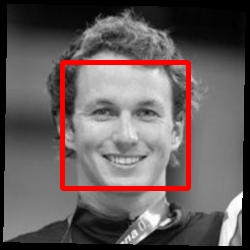
\includegraphics[width=\textwidth]{conflitos/correcta}
                \caption{Correcta}
                \label{fig:conflitos-correcta}
        \end{subfigure}%
        ~ 
        \begin{subfigure}[b]{0.2\textwidth}
                \centering
                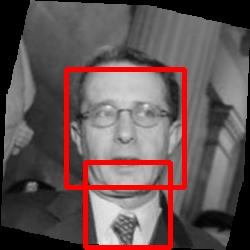
\includegraphics[width=\textwidth]{conflitos/falsos_positivos}
                \caption{Falso Positivo}
                \label{fig:conflitos-falsos_positivos}
        \end{subfigure}
        ~ 
        \begin{subfigure}[b]{0.2\textwidth}
                \centering
                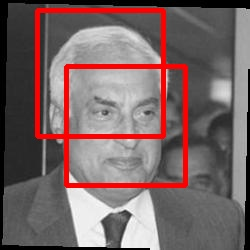
\includegraphics[width=\textwidth]{conflitos/multiplas_areas}
                \caption{Múltiplas Áreas}
                \label{fig:conflitos-multiplas_areas}
        \end{subfigure}
        ~ 
        \begin{subfigure}[b]{0.2\textwidth}
                \centering
                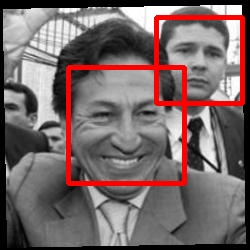
\includegraphics[width=\textwidth]{conflitos/multiplas_faces}
                \caption{Múltiplas Faces}
                \label{fig:conflitos-multiplas_faces}
        \end{subfigure}
        \caption{Comparação entre face correctamente detectada e situações de erro na detação}\label{fig:conflitos-detecao}
\end{figure}

Para uma dada imagem, a tarefa de deteção da face é responsável pela determinação de uma área de interesse, de forma rectangular, onde se encontra a face que se pretende fornecer às etapas de treino ou teste do sistema Visage. Um exemplo de uma imagem cuja face foi corretamente detetada e da respetiva área de interesse, assinada a vermelho, pode ser encontrado na Figura \ref{fig:conflitos-correcta}.

Apesar do bom desempenho do classificador utilizado na deteção das faces presentes nas imagens, existem algumas situações onde se verificou a existência de erros ou conflitos nos resultados obtidos, tal como ilustrado na Figura  \ref{fig:conflitos-detecao}. De seguida encontram-se descritas as três situações de erro encontradas:
\begin{description}
\item[Falsos Positivos] Zonas da imagem que não contém faces podem ser assinaladas como área de interesse, tal como ilustrado na Figura \ref{fig:conflitos-falsos_positivos};
\item[Múltiplas Áreas de Interesse] Para a mesma face, na análise de uma imagem são devolvidas várias regiões de interesse, tal como pode ser visto na Figura \ref{fig:conflitos-multiplas_areas};
\item[Múltiplas Faces] Na galeria utilizada para o desenvolvimento e avaliação do sistema, LFW-a, existem situaçoes onde mais do que uma pessoa se encontra representada na mesma imagem, no entanto, em cada imagem é apresentada apenas a anotação textual para a face mais relevante na fotografia, tal como pode ser visto na Figura \ref{fig:conflitos-multiplas_faces}, onde apenas a face maior possui uma anotação textual associada, pelo que apenas essa face deve ser extraída da imagem.
\end{description}

\begin{table}
\caption{Resultados etapa de de deteção facial para todas as pessoas com pelo menos 2 imagens na biblioteca LFW-a.}
    \begin{tabular}{ll}
    \hline
    \hline
    Pessoas                                                 & 1680                   \\
    Imagens                                                 & 9165                   \\ \hline
    Imagens com faces detectadas s/ conflito                & 95.50\% (8753 imagens) \\
    Conflitos e falsos positivos resolvidos automaticamente & 1.63\% (149 imagens)   \\
    Conflitos e falsos positivos não resolvidos (empates)   & 0.34\% (31 imagens)    \\
    Imagens com faces não detectadas                        & 2.52\% (231 imagens)   \\
    \hline
    \hline
    \end{tabular}
    \label{tab:desempenho_detecao}
\end{table}

Para a remoção dos casos de conflito observados na deteção das faces presentes na biblioteca LFW-a e ilustrados na Figura \ref{fig:conflitos-detecao}, foi adoptada a seguinte estratégia:

Para uma dada imagem é verificada a existência de uma cara usando o classificador em cascata treinado para o reconhecimento de caras frontais. Caso se verifique a deteção de um conflito, nessa imagem é necessário proceder à re-avaliação de cada uma das regiões assinaladas como área de interesse, de forma a determinar em qual se encontra a face que se pretender utilizar.

Na avaliação das várias regiões de interesse é procurada a existência de olhos, boca e nariz, com recurso a três classificadores em cascata treinados para o reconhecimento de cada um destes componentes em específico. Posteriormente é calculada uma pontuação para cada uma das regiões de interesse conforme os elementos encontrados:
\begin{itemize}
\item +100 Pontos caso sejam encontrados o par de olhos (olho esquerdo e direito) na face;
\item +50 Pontos caso seja encontrada a boca. No caso de terem sido encontrados previamente os olhos, é também verficado se distância entre a boca e os olhos é de de pelo menos 20 píxeis, de modo a garantir que um olho não é classificado como boca e vice-versa;
\item + 50 Pontos caso seja encontrado o nariz na face.
\end{itemize}
A pontuação de uma região de interesse varia assim entre os 0 e os 200 pontos. No final, é guardada apenas a região de interesse com maior pontuação. Em caso de empate, são guardadas ambas as regiões de interesse, e o utilizador do sistema é avisado do conflito, o qual deverá ser resolvido posteriormente de forma manual.

O desempenho da tarefa de deteção facial numa amostra da biblioteca LFW-a, pode ser visualizado na Tabela \ref{tab:desempenho_detecao}. Nesta amostra foram incluídas apenas as fotografias de pessoas que tenham pelos menos 2 imagens na biblioteca LFW-a, uma vez que apenas essas poderão ser utilizadas na avaliação do desempenho do sistema, utilizando, pelo menos, uma imagem para treino e uma imagem para teste. Tal como é possível observar o desempenho desta etapa é muito satisfatório, sendo que 95.5\% das faces imagens presentes nas imagens são detetadas automaticamente, às quais acrescentem 149 imagens para as quais foi possível resolver automaticamente os conflitos detetados, resultando num total de 97.13\% de faces corretamente detetadas.

\subsection{Alinhamento e Corte} \label{sec:alinhamentoEcorte}
A tarefa de deteção face é responsável pela determinação de uma região de interesse na imagem original onde se encontra a face, sendo essa região correspondente a um retângulo tal como ilustrado na Figura \ref{fig:conflitos-correcta}. Após a deteção da região de interesse onde se encontra a face, é então possível proceder ao seu alinhamento e corte através da seguinte estratégia:

\begin{enumerate}
\item Utilizando um classificador em cascata existente na biblioteca \textit{OpenCV} é verificada a posição do olho esquerdo na região de interesse determinada para a face;
\item Utilizando um classificador em cascata existente na biblioteca \textit{OpenCV} é verificada a posição do olho direito na região de interesse determinada para a face;
\item São removidos conflitos e falsos positivos nas posições obtidas para o olho esquerdo e direito (ver Sub-secção seguinte), obtendo-se assim as duas regiões mais prováveis para cada um dos olhos;
\item É calculado o ponto central das regiões determinadas como mais prováveis para o olho esquerdo e direito, em que $p_{esquerdo}(x_1,y_1)$ corresponde ao ponto central da região detetada para o olho esquerdo, e  $p_{direito}(x_2,y_2)$ corresponde ao ponto central da região detetada para o olho direito.
\item É calculado o ângulo de rotação da imagem ($\theta$), a partir da posição determinada para os olhos:
\begin{equation}
\theta = \arctan(x_1 - x_2, y_1 - y_2)
\end{equation}
\item A imagem é rodada de acordo com o ângulo de rotação $\theta$ calculado.
\item A imagem é cortada de acordo com a região de interesse determinada na tarefa de deteção face.
\end{enumerate}

Caso não se pretenda efetuar o alinhamento da face, mas apenas a sua segmentação da restante imagem, como se verifica na utilização da galeria já alinhada, LFW-a, na avaliação do desempenho do sistema, os passos 1 a 6 são ignorados, sendo apenas segmentada a imagem de acordo com a região de interesse determinada na tarefa de deteção face. Na Figura \ref{fig:alinhamentos} encontra-se representada uma comparação entre uma imagem apenas recortada, a mesma imagem alinhada e recortada pelas estratégias acima descritas e ainda as versões LFW e LFW-a dessa imagem.

\begin{figure}[t]
        \centering
        \begin{subfigure}[b]{0.2\textwidth}
                \centering
                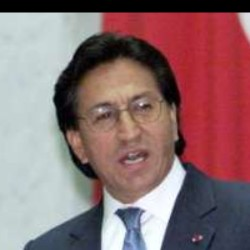
\includegraphics[width=\textwidth]{alinhamentos/original}
                \caption{LFW-Original}
                \label{fig:alinha_original}
        \end{subfigure}%
        ~ 
        \begin{subfigure}[b]{0.2\textwidth}
                \centering
                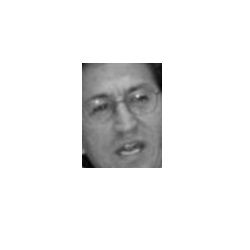
\includegraphics[width=\textwidth]{alinhamentos/nao-alinhada}
                \caption{Recortada}
                \label{fig:alinha_nao-alinhada}
        \end{subfigure}
        ~ 
        \begin{subfigure}[b]{0.2\textwidth}
                \centering
                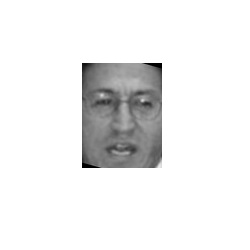
\includegraphics[width=\textwidth]{alinhamentos/alinhada}
                \caption{Alinhada}
                \label{fig:alinha_alinhada}
        \end{subfigure}
        ~ 
        \begin{subfigure}[b]{0.2\textwidth}
                \centering
                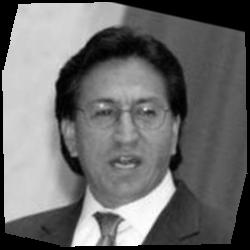
\includegraphics[width=\textwidth]{alinhamentos/lfw-a}
                \caption{LFW-a}
                \label{fig:alinha_lfw-a}
        \end{subfigure}
        \caption{Comparação entre versões original, recortada, alinhada e LFW-a.}\label{fig:alinhamentos}
\end{figure}

\subsubsection*{Remoção de Conflitos e Falsos Positivos}
Tal como explicado anteriormente, a necessidade de alinhamento de uma face previamente detetada é calculada com base na localização estimada para o seu olho esquerdo e direito e a inclinação da reta formada pela intersecção dos dois pontos centrais de cada um dos olhos. Para detetar um olho, à semelhança da estratégia adotada para detetar uma face, é utilizado um classificador em cascata que devolve uma região rectangular onde é provável a existência de um olho. 

A morfologia de um olho é um caso particularmente difícil de deteção, tendo-se registado a existência de um grande número de falsos positivos para os classificadores utilizados (olho esquerdo e direito), assim como uma má diferenciação entre o olho esquerdo, direito e a boca em algumas das imagens, pelo que a adoção de uma estratégia de remoção de conflitos se revelou essencial para a conclusão desta tarefa de pré-processamento com sucesso. A estratégia adotada foi a seguinte:

Seja $w$ a largura de uma imagem de face a alinhar e $h$ a sua altura. Sejam $c_{esquerdo}(x_1,y_1)$ e  $c_{direito}(x_2,y_2)$  os pontos correspondentes aos cantos superiores esquerdos das regiões de interesse detetadas para o olho esquerdo e direito, respetivamente, e $w_{esquerdo}$, $w_{direito}$, $h_{esquerdo}$ e $h_{direito}$ a largura e altura dessas mesmas regiões. Os conflitos entre as diversas regiões de interesse devolvidas pelos classificadores utilizados são removidos através da utilização das seguintes restrições:

\begin{itemize}
\item $x_1 < \frac{w}{4}$ e $\frac{w}{4} < x_2 < \frac{3\times w}{4}$;
\item $y_1 < \frac{h}{2}$ e $y_2 < \frac{h}{2}$;
\item $w_{esquerdo} < \frac{5\times w}{8}$ e $w_{direito} < \frac{5\times w}{8}$;
\item $h_{esquerdo} < \frac{h}{2}$ e $h_{direito} < \frac{h}{2}$;
\end{itemize}

\subsection{Normalização do Contraste} \label{sec:normalizacao}

Tal como destacado na Secção \ref{sec:sub-problemas} a tarefa de normalização encontra-se presente em alguns sistemas de reconhecimento facial automático com o objetivo de melhorar os resultados obtidos independentemente de fatores como a iluminação ou pose das faces nas imagens. A tarefa de normalização do contraste de imagem tem como objetivo normalizar a face no que diz respeito à sua iluminação e aumentar o contraste existente na mesma. De forma a tornar o sistema versátil e analisar o impacto de diferentes estratégias foram utilizadas as seguintes alternativas, ilustradas na Figura \ref{fig:normalizacao}, para a normalização do contraste:

\begin{figure}[t]
        \centering
        \begin{subfigure}[b]{0.2\textwidth}
                \centering
                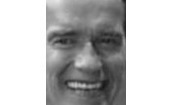
\includegraphics[width=\textwidth]{normalizacao/original}
                \caption{Original               }
                \label{fig:normalizacao-original}
        \end{subfigure}%
        ~
        \begin{subfigure}[b]{0.2\textwidth}
                \centering
                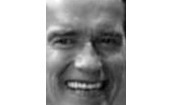
\includegraphics[width=\textwidth]{normalizacao/normalized}
                \caption{\textit{C. Streching}}
                \label{fig:normalizacao-normalized}
        \end{subfigure}
        ~ 
        \begin{subfigure}[b]{0.2\textwidth}
                \centering
                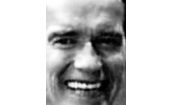
\includegraphics[width=\textwidth]{normalizacao/equalized}
                \caption{Equalização H.}
                \label{fig:normalizacao-equalized}
        \end{subfigure}
        ~
        \begin{subfigure}[b]{0.2\textwidth}
                \centering
                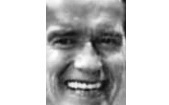
\includegraphics[width=\textwidth]{normalizacao/clahe}
                \caption{\textit{CLAHE}}
                \label{fig:normalizacao-clahe}
        \end{subfigure}
        ~ 
        \caption{Comparação entre imagem original e as várias técnicas de normalização disponíveis.}\label{fig:normalizacao}
\end{figure}

\begin{description}
\item[\textit{Contrast Streching}]
A técnica de \textit{Contrast Streching}, também designada por alguns autores simplesmente de normalização, consiste numa tentativa de alargar a gama de valores utilizados para codificar a intensidade de uma imagem de forma a que seja utilizada toda a gama de valores possíveis. No sistema desenvolvido as imagens utilizadas encontram-se convertidas para tons de cinzento, pelo que a normalização efetuada consiste num mapeamento linear dos valores originais para uma gama de intensidade entre 0 e 255. Um exemplo de uma face normalizada segundo esta estratégia pode ser visualizado na imagem \ref{fig:normalizacao-normalized}.
\end{description}

\begin{description}
\item[Equalização Histograma]
O histograma de uma imagem descreve a distribuição estatística dos níveis de intensidade de uma imagem, neste caso concreto dos níveis de cinzento, em função do seu número de píxeis. A equalização do histograma de uma imagem consiste no mapeamento das variações da escala de cinzentos de forma a que o histograma resultante se aproxime de uma outra distribuição, mais alargada e idealmente uniforme na distribuição dos valores de intensidade da imagem. Este procedimento parte do princípio de que a qualidade da imagem é uniforme em toda a imagem, aplicando um mapeamento similar a toda a imagem \cite{Bradski2008}. Um exemplo de uma imagem cujo histograma foi equalizado pode ser visto na Figura \ref{fig:normalizacao-equalized}.
\end{description}

\begin{description}
\item[\textit{CLAHE}]
\textit{Contrast limited adaptive histogram equalization (CLAHE)} procura ultrapassar as limitações da equalização de contraste, através de uma abordagem local ao problema de normalização do histograma de uma imagem. Ao contrário da abordagem tradicional apresentada acima, esta técnica tem em conta a intensidade de um conjunto de píxeis e dos seus vizinhos para a normalização do contraste e não a intensidade de toda a imagem. Para além disso, tal como o seu nome indica, esta abordagem incluí ainda um limite para o qual a equalização do histograma é realizada, evitando assim o mapeamento demasiado agressivo quando duas escalas de intensidade dispares se encontram na mesma região \cite{Reza2004}. Na Figura \ref{fig:normalizacao-clahe} encontra-se representada uma imagem resultante da sua normalização através da técnica CLAHE.
\end{description}

\subsection{Aplicação Filtro Abstração} \label{sec:filtros}
A quarta etapa de pré-processamento efetuada no sistema Visage corresponde à aplicação de um filtro de abstração sobre uma imagem. Os filtros de abstração constituem uma forma moderna de simplificação de conteúdo visual, com a sua utilização no âmbito do sistema Visage, pretendemos analisar o seu impacto no processo de reconhecimento.

Encontram-se disponíveis três filtros, Gaussiano, Bilateral e Kuwahara Anisotrópico, os quais constituem três níveis de abstração sucessivamente mais complexos. A abstração efetuada para cada filtro encontra  ilustrada na Figura \ref{fig:filters}, apresentado-se de seguida uma breve descrição de cada um dos filtros utilizados:

\begin{figure}[t]
        \centering
        \begin{subfigure}[b]{0.2\textwidth}
                \centering
                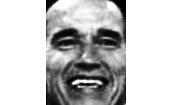
\includegraphics[width=\textwidth]{filters/original}
                \caption{Original}
                \label{fig:filters-original}
        \end{subfigure}%
        ~
        \begin{subfigure}[b]{0.2\textwidth}
                \centering
                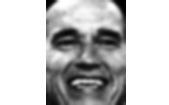
\includegraphics[width=\textwidth]{filters/gaussian}
                \caption{Gaussiano}
                \label{fig:filters-gaussian}
        \end{subfigure}
        ~ 
        \begin{subfigure}[b]{0.2\textwidth}
                \centering
                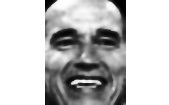
\includegraphics[width=\textwidth]{filters/bilateral}
                \caption{Bilateral}
                \label{fig:filters-bilateral}
        \end{subfigure}
        ~
        \begin{subfigure}[b]{0.2\textwidth}
                \centering
                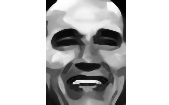
\includegraphics[width=\textwidth]{filters/akf}
                \caption{Kuwahara A.}
                \label{fig:filters-kuwahara}
        \end{subfigure}
        ~ 
        \caption{Comparação entre imagem original e os vários filtros de abstração utilizados.}\label{fig:filters}
\end{figure}

\begin{description}
\item[Filtro Gaussiano]
A aplicação de um filtro gaussiano para a suavização de uma imagem é uma técnica amplamente utilizada em áreas próximas do processamento de imagem e computação gráfica e tem como objetivo reduzir o ruído e detalhe de uma imagem. Um filtro gaussiano calcula um média pesada dos valores dos píxeis vizinhos, na qual o peso de um píxel na média diminui conforme a sua distância ao centro aumenta.

No âmbito do sistema Visage a utilização deste filtro tirou partido da implementação existente na biblioteca \textit{OpenCV}, nomeadamente a partir da função \textit{gaussianBlur}, tendo sido utilizada uma vizinhança de raio sete píxeis.

\item[Filtro Bilateral]
Tal como introduzido na Secção \ref{subsec:bilateral}, o filtro bilateral tem como objetivo suavizar as zonas com menor contraste na imagem sem afetar os limites de maior contraste, permitindo assim reduzir o ruído presente na imagem enquanto os seu contornos são preservados.

À semelhança do filtro gaussiano a utilização deste filtro foi efetuada com recurso à implementação existente na biblioteca \textit{OpenCV}, nomeadamente a partir da função \textit{bilateralFilter}, tendo sido utilizado um raio de oito píxeis vizinhos na aplicação do filtro.

\item[Filtro Kuwahara Anisotrópico]
O filtro Kuwahara Anisotrópico (FKA) é uma generalização do filtro Kuwahara (ver \ref{subsec:kuwahara}) que remove alguns artefactos originados na aplicação do filtro original através da adaptação da forma, escala e orientação do filtro à estrutura local das características da imagem \cite{Kyprianidis2009}. Desta forma é produzido um efeito de abstração tipo pintura, onde é removida informação não essencial em zonas de elevado contraste, enquanto são preservados os limites representados nas zonas de menor contraste. As imagens ficam assim com a clareza de uma ilustração, mas preservam a informação direcional tal como nas pinturas a óleo clássicas. Por outro lado, este filtro tira partido da placa gráfica para a realização da abstração das imagens, tornando-se assim particularmente indicado para o processamento de um elevado número de fotografias.

Para a utilização deste filtro foi utilizada a implementação de Jan Kyprianidis disponível em [] \footnote{https://code.google.com/p/gpuakf/}.

\end{description}
\subsection{Aplicação de Máscara} \label{sec:mascara}

\begin{figure}[t]
        \centering
        \begin{subfigure}[b]{0.2\textwidth}
                \centering
                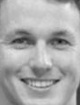
\includegraphics[width=\textwidth]{mascara/sem_mascara}
                \caption{Original}
                \label{fig:sem-mascara}
        \end{subfigure}%
        ~ ~ ~
        \begin{subfigure}[b]{0.2\textwidth}
                \centering
                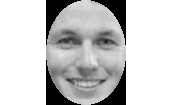
\includegraphics[width=\textwidth]{mascara/com_mascara}
                \caption{Recortada}
                \label{fig:com-mascara}
        \end{subfigure}
        ~ 
        \caption{Exemplo de face já segmentada, com e sem máscara.}\label{fig:mascara}
\end{figure}

A existência de fundo e elementos externos à face numa imagem pode afetar significativamente os resultados obtidos no seu reconhecimento ao permitir que um conjunto de imagens com fundos semelhantes possam ser identificadas como pertencendo à mesma pessoa não pela face representada na imagem, mas pelos elementos presentes no fundo da mesma. A aplicação de uma máscara elíptica sobre face visa a remoção do fundo ainda existente na imagem após a deteção e segmentação da face e eventuais tarefas de pré-processamento realizadas.

Um exemplo de uma imagem antes e depois da aplicação da máscara pode ser visto em \ref{fig:mascara}. A estratégia de aplicação de uma máscara para melhoria dos resultados obtidos no reconhecimento facial já foi aplicada com sucesso anteriormente em diversas situações, como são exemplo a avaliação FERET \cite{Phillips2000} ou o trabalho realizado por Ahonen \textit{et al.} \cite{ahonen2004face}.

\section{Módulo \textit{FaceModel}} \label{sec:facemodel}
O módulo \textit{FaceModel} constitui uma camada de nível superior implementada para encapsular a comunicação com módulo de reconhecimento facial disponível na biblioteca \textit{OpenCV}, designado \textit{FaceRecognizer}, assim como estender algumas das funcionalidades do mesmo. 

As principais responsabilidades do módulo \textit{FaceModel} consistem em criar e treinar de um modelo de reconhecimento facial, assim como determinar para uma dada imagem qual a sua identificação mais provável, ou qual o conjunto ordenado de identificações mais prováveis a partir do modelo criado.

O modelo de reconhecimento facial pode ser criado com três algoritmos de reconhecimento facial diferentes, \textit{Eigenfaces}, \textit{Fisherfaces} e \textit{LBPH}, implementados na biblioteca OpenCV e descritos em mais pormenor nas secções \ref{sec:eigen}, \ref{sec:fisher} e \ref{sec:lbph}, respetivamente. Uma vez treinado um modelo é também possível armazenar o mesmo num ficheiro e carrega-lo posteriormente, evitando assim um novo treino, o qual dependendo do número de imagens a treinar pode revelar-se computacionalmente custoso.

As funcionalidades disponíveis na biblioteca \textit{OpenCV} para os três algoritmos implementados foram expandidas no de forma a permitir que, para uma dada imagem fornecida ao sistema, seja devolvida uma lista ordenada, por ordem crescente de similaridade, de entidades. Desta forma é possível para além de identificar a pessoa presente numa imagem, dizer qual a lista de pessoas que mais se parecem com a pessoa representada na imagem. Uma descrição detalhada da expansão efetuada às funcionalidades disponíveis na biblioteca OpenCV pode ser encontrada em \ref{sec:topn}.

\subsection{\textit{Eigenfaces}} \label{sec:eigen}
O método \textit{Eigenfaces} foi introduzido por Turk e Pentland em 1991 \cite{Turk1991}, e tira partido da Análise dos Componentes Principais (ACP) para efetuar o reconhecimento facial automático.

A análise de componentes principais tem como objetivo determinar as relações existentes entre diferentes conjuntos de dados, nomeadamente ao nível das suas diferenças e semelhanças, tirando partido da redundância existente para criar uma representação reduzida dos dados sem que a perda de informação ocorrida seja significativa. As imagens faciais possuem uma grande redundância natural, o algoritmo \textit{Eigenfaces}, através da análise dos componentes principais dessas imagens, efetua uma projeção das imagens faciais num sub-espaço onde se evidenciam apenas as variações entre as diversas caras conhecidas pelo sistema.

A redução do espaço de representação revela-se fulcral no problema de reconhecimento facial em imagens, devido à grande dimensionalidade exigida para a representação de uma face. Considerando, por exemplo, uma dada imagem de $n$ x $m$ píxeis de tons cinzentos, essa imagem poderia ser traduzida por um espaço vetorial de $m = $ $n$ x $m$ píxeis, assim sendo, uma imagem de apenas $256x256$ píxeis necessitaria de um total de $65536$ píxeis para ser representada.

O processo de reconhecimento facial com recurso ao algoritmo \textit{Eigenfaces} consiste nos seguintes passos:
\begin{enumerate}
\item Aquisição de um conjunto de dados iniciais (conjunto de treino);
\item Projeção dos dados obtidos num sub-espaço de faces através da ACP;
\item Aquisição de uma imagem a reconhecer;
\item Projeção da face a reconhecer no sub-espaço do conjunto de treino, calculando as distâncias obtidas para cada face conhecida pelo sistema;
\item Determinar qual a face do conjunto de treino com menor distância à face a reconhecer;
\item Caso a distância para a face obtida seja menor do que um limite operacional estabelecido, a imagem é reconhecida como sendo essa pessoa, caso contrário, a face é identificada como sendo uma pessoa desconhecida pelo sistema.
\end{enumerate}

Este método efetua assim uma abordagem holística ao problema de reconhecimento facial em imagens, uma vez que tem em consideração a representação facial como um todo, não fazendo a distinção entre pontos específicos da face como olhos, orelhas ou nariz para efetuar o reconhecimento facial. Uma vantagem deste tipo de representação é a reduzida sensibilidade ao ruído presente nas imagens \cite{Zhao2003}.

\subsection{\textit{Fisherfaces}} \label{sec:fisher}
A análise dos componentes principais visa determinar o sub-espaço onde se verifica uma maior variação entre um conjunto de imagens. No entanto, a variação na representação facial de uma pessoa encontra-se muitas vezes relacionada com mudanças de expressões faciais ou iluminação dos indivíduos, pelo que, o sub-espaço criado pelo algoritmo \textit{Eigenfaces} não traduz muitas vezes apenas as diferenças de identidade entre os diversos indivíduos, mas também as diferenças verificadas entre as várias representações de um indivíduo devido à variação nas condições de captura das imagens. O algoritmo \textit{Fisherfaces} \cite{Belhumeur1997, Etemad1997, Zhao1998}, tenta resolver este problema, através da aplicação de um passo de Análise Linear Discriminante (ALD) \textit{(Linear Discriminant analysis)} após a análise dos componentes principais, de forma a determinar mais corretamente as variações intra-classe existentes no conjunto de imagens a avaliar.

A ALD, inicialmente introduzida por Fisher em 1936 \cite{FISHER1936}, tenta maximizar as diferenças existentes entre diferentes indivíduos(inter-classe) e minimizar as variações entre imagens da mesma pessoa(intra-classe) de modo a obter uma representação mais robusta em termos de variação ao nível da iluminação. Após a aplicação dos passos de ACP e ALD, o processo de reconhecimento do método \textit{Fisherfaces} é semelhante ao efetuado pelo método \textit{Eigenfaces}, sendo também efetuada uma abordagem holística ao reconhecimento facial.


\subsection{\textit{Local Binary Patterns Histograms (LBPH)}} \label{sec:lbph}
Ao contrário dos algoritmos descritos anteriormente, o LBPH efetua uma abordagem local ao problema de reconhecimento facial, efetuando uma extração das características locais de uma imagem. Este tipo de abordagem possuí a vantagem de possuir uma baixa dimensionalidade implícita, pelo que não existe a necessidade de efetuar a projeção das imagens num sub-espaço.

A ideia base das \textit{Local Binary Patterns (LBP)}, consiste em resumir a estrutura local de imagem através de uma comparação de um píxel com os seus vizinhos. Dado um píxel central é analisada a diferença entre esse píxel e cada um dos seus vizinhos. Se a intensidade do píxel for maior ou igual do que a do seu vizinho é atribuído o valor 1, caso contrário é atribuído o valor 0. Cada píxel pode então ser traduzido por um número binário do género $11001111$. Dados $8$ píxeis é então possível efetuar $2^8$ combinações, cada uma designada de LBP.

Ahonen \textit{et al.} \cite{ahonen2004face}, propuseram o uso de LBP para o reconhecimento facial em imagens. A sua abordagem consiste na divisão da face em pequenas regiões das quais são derivadas LBP e concatenadas numa representação única designada de LBPH, a qual representa uma imagem facial. O reconhecimento é depois efetuado através do determinação do vizinho mais próximo no espaço de faces computado.

\subsection{Top $N$ Resultados} \label{sec:topn}
Após o treino do sistema, a identificação de uma imagem é obtida de forma semelhante para os três algoritmos disponíveis, e pode ser resumida no seguinte conjunto de passos:
\begin{enumerate}
\item É criada uma representação de baixo nível da imagem a identificar, aqui designada de prova.
\item A prova é comparada a cada uma das representações de baixo nível criadas durante o treino do sistema e às quais se encontra associado um código numérico representativo da pessoa associada a essa representação.
\item É devolvida o código da pessoa correspondente à menor distância entre a prova e a representação de baixo nível treinada.
\end{enumerate}

Para os algoritmos \textit{Eigenfaces} e \textit{Fisherfaces} a representação de baixo nível de uma imagem corresponde à projeção desta no sub-espaço de imagens criado com a análise dos componentes principais, no caso do \textit{Eigenfaces}, e com a posterior análise linear discriminante, no caso do \textit{Fisherfaces}. A comparação entre a prova e as representações de baixo nível criadas no treino é efetuada em ambos os casos através da distância euclidiana entre as matrizes das duas representações.

Para o algoritmo \textit{LBPH} a representação de baixo nível criada corresponde ao histograma representativo das \textit{local binary patterns} de uma imagem. A comparação entre a prova e as representações de baixo nível criadas durante o treino é efetuada através da comparação da distância entre os seus histogramas.

A extensão efetuada à implementação existente na biblioteca \textit{OpenCV}, incide sobre o ponto 3 dos passos acima citados. Em vez de apenas ser devolvido o código identificativo da pessoa cuja representação apresenta menor distância às representações de baixo nível existentes, é devolvida uma lista de $n$ elementos, ordenada de forma crescente pelas distâncias calculadas. Esta lista encontra-se agrupada pelas diferentes entidades, significando assim que cada pessoa apenas aparece uma única vez na lista, independentemente, ou não da existência de várias representações de baixo nível referentes a essa pessoa. Desta forma torna-se possível o desenvolvimento de aplicações que, da uma imagem, respondam às perguntas "Qual é nome das 10 pessoas mais parecidas com a imagem fornecida?" em vez de apenas "Qual é a pessoa mais parecida com a imagem fornecida?".

\section{Funcionalidades}
O trabalho realizado no âmbito desta dissertação resultou na criação de cinco executáveis com diferentes funcionalidades e responsabilidades no âmbito do sistema Visage. Os primeiros três \textit{FaceDetector.exe}, \textit{FaceRecognizer.exe} e \textit{CSVCreator.exe} foram utilizados para efetuar a avaliação reportada no Capítulo \ref{chap:resultados}. Já os programas \textit{TrainAndSaveModel.exe} e \textit{TopN.exe} permitem a utilização do sistema Visage como base de outros programas que tirem partido do reconhecimento facial de imagens no seu funcionamento.

\begin{description}
\item[FaceDetector.exe] Efetua o pré-processamento de uma galeria de imagens de acordo com os seguintes argumentos:

\begin{itemize}
\item \textbf{\textit{libraryPath.txt}}: O ficheiro txt com a descrição das imagens da galeria a processar.
\item \textbf{\textit{outputDirName}}: O caminho do novo diretório a criar.
\item \textbf{-mask}: Define se deve ser colocada uma máscara sobre a imagem (ver \ref{sec:mascara}). Parâmetro opcional.
\item \textbf{\textit{-N, -E ou -C}}: Define qual o tipo de normalização que deve ser efetuada sobre a imagem, \textit{-N}, \textit{-E} ou \textit{-C} para as técnicas \textit{Contrast Streching}, Equalização Histograma e CLAHE, respetivamente (ver \ref{sec:normalizacao}). Parâmetro opcional.
\item \textbf{\textit{-G ou -B}}: Define qual o filtro de abstração a aplicar sobre a imagem, -G ou -B, para os filtros gaussiano ou bilateral, respetivamente. Para efetuar o pré-processamento com recurso ao filtro kuwahara anisotrópico é necessário recorrer a um programa externo (ver \ref{sec:filtros}). Parâmetro opcional.
\item \textbf{\textit{-align}}: Define se deve ser efetuado alinhamento das faces detetadas nas imagens (ver \ref{sec:alinhamentoEcorte}). Parâmetro opcional.
\end{itemize}

\item[FaceRecognizer.exe] Efetua a avaliação do desempenho do sistema de reconhecimento facial para uma determinada galeria, de acordo com os seguintes parâmentros:

\begin{itemize}
\item \textbf{\textit{libraryPath.txt}}: O ficheiro txt com a descrição das imagens da galeria a processar.
\item \textbf{\textit{results.txt}}: O ficheito txt com os resultados da avaliação efetuada num formato legível para humanos.
\item \textbf{\textit{-E, -F ou -L}}: Define qual o algoritmo de reconhecimento facial a utilizar -E, -F ou -L para \textit{Eigenfaces}, \textit{Fisherfaces} ou \textit{LBPH} (ver \ref{sec:facemodel}).
\item \textbf{\textit{nResults }}: Define o número de rankings máximo a avaliar.
\end{itemize}

\item[CSVCreator.exe] Permite criar novas sub-galerias a partir de outras pré-existentes, assim como computar as estatísticas de uma galeria, de acordo com os seguinte parâmetros:

\begin{itemize}
\item \textbf{\textit{libraryPath.txt}}: O ficheiro txt com a descrição das imagens da galeria original.
\item \textbf{\textit{outputfilename}}: O nome do ficheiro com a descrição da sub-galeria criada.
\item \textbf{\textit{bottomLimit}}: O número de mínimo de imagens por pessoa.
\item \textbf{\textit{topLimit}}: O número de máximo de imagens por pessoa.
\item \textbf{\textit{statsFile}}: Nome do ficheiro onde ficam armazenadas as estatísticas de uma galeria.
\end{itemize}

\item[TrainAndSaveModel.exe] Permite treinar um modelo de reconhecimento facial de uma galeria passada como argumento e grava-lo para um ficheiro para posterior utilização.

\begin{itemize}
\item \textbf{\textit{libraryPath.txt}}: O ficheiro txt com a descrição das imagens da galeria a processar.
\item \textbf{\textit{percentageToTrain}}: A percentagem de imagens de cada pessoa a usar como imagem de treino e teste.
\item \textbf{\textit{-E, -F ou -L}}: Define qual o algoritmo de reconhecimento facial a utilizar -E, -F ou -L para \textit{Eigenfaces}, \textit{Fisherfaces} ou \textit{LBPH} (ver \ref{sec:facemodel}).
\item \textbf{\textit{output.xml}}: O ficheiro onde deve ser gravado o modelo treinado.
\end{itemize}

\item[topN.exe] Devolve o nomes das \textit{n} personalidades mais parecidas com a personalidade representada na imagem. Efetua o pré-processamento da imagem passada como argumentos, com aplicação de máscara, normalização através de equalização do histograma e alinhamento da face.

\begin{itemize}
\item \textbf{\textit{imagePath}}: O caminho da imagem a reconhecer.
\item \textbf{\textit{model.xml}}: O modelo de reconhecimento facial previamente treinado a utilizar.
\item \textbf{\textit{nResults}}: O número de elementos máximo a incluir no top de resultados devolvido.
\end{itemize}

\end{description}
\chapter{Avaliação e Resultados} \label{chap:resultados}
\textbf{FALTA FAZER ESTE TEXTO}
\textbf{FALTA REFERIR MAQUINAS UTILIZADAS}

A hipótese levantada no âmbito desta dissertação é que o uso de abstração em imagens que vão ser ser alvo de reconhecimento facial pode melhorar o processo de reconhecimento facial automático em imagens. Para a análise desta hipótese foi criado um sistema de reconhecimento facial automático em imagens, assim  como, escolhida uma biblioteca de imagens a analisar, tal como descrito em \ref{chap:visage}. Neste capítulo, é apresentada a metodologia de avaliação adotada para a análise da hipótese levantada, assim como do sistema de reconhecimento facial Visage e são também apresentados os resultados obtidos.



-Definição da coleção base a analisar

-Definição de quais os conjuntos de teste a criar a partir da coleção base

-Definição das experiências que se pretendem realizar e porquê

-Forma de avaliar e resultados dessas experiências

O desempenho de sistemas de reconhecimento facial pode ser analisado através de diferentes perspetivas, tal como introduzido na secção \ref{sec:problema} desta dissertação. A biblioteca LFW foi criada com o propósito inicial da análise do sub-problema de reconhecimento facial \textit{pair matching}, no qual o sistema deve decidir se duas faces representam ou não o mesmo indivíduo. No entanto, as características desta biblioteca, nomeadamente no que diz respeito à existência da anotação textual das pessoas presentes em cada imagem, à existência de apenas uma pessoa representada (de forma relevante) em cada imagem e ainda da normalização do formato das imagens, permitem que esta biblioteca possa ser utilizada com um esforço reduzido para o analise dos restantes sub-problemas de reconhecimento facial automático.

No âmbito desta dissertação temos em vista a realização de um conjunto de experiências descritas em \ref{sec:experiencias} e análise dos seus resultados através de duas perspetivas descritas nos pontos \ref{sec:avaliacao1} e \ref{sec:avaliacao2} a seguir. Uma vez que estas avaliações não se encontram enquadradas no paradigma de avaliação de \textit{pair matching}, para o qual a biblioteca LFW foi originalmente criada tornou-se necessário a criação de novos conjuntos de teste, os quais passamos a apresentar de seguida.

As imagens dos conjuntos de testes descritos em \ref{sec:conjuntos} foram sujeitas a um conjunto de tarefas de pré-processamento, descritas em \ref{sec:experiencias}, resultado na criação de um conjunto de galerias de imagens pré-processadas, as quais se encontram resumidas na tabela \ref{tab:colecoes}. Todas as galerias resultantes possuem as mesmas imagens, diferenciando-se apenas pelas tarefas de pré-processamento a que foram sujeitas.

Nesta secção encontram-se reportados os resultados da avaliação efetuada ao desempenho do sistema de reconhecimento facial Visage.

A qualidade do desempenho de um sistema de reconhecimento facial automático, assim como a satisfação dos seus utilizadores está intimamente relacionada com o fim para o qual o sistema foi criado. No âmbito desta dissertação, a avaliação do desempenho foi efetuada segundo duas perspetivas distintas, \textit{Closed-set Identification} e \textit{Image Retrieval}, as quais são apresentadas de seguida. A primeira constitui uma medida padrão de avaliação do desempenho de sistemas de reconhecimento facial automático, a segunda, pretende analisar o desempenho do sistema de um ponto de vista mais próximo de um provável caso de uso, neste caso, \textit{Image Retrieval}.


\section{Conjuntos de Teste}  \label{sec:conjuntos}

Na avaliação de sistemas de reconhecimento facial automáticos designam-se de \textit{amostras biométricas} as capturas de características de uma pessoa que permitem efetuar o seu reconhecimento. Dependendo do sistema, as amostras biométricas podem ser apenas uma imagem, um conjunto de imagens, ou um vídeo. No projeto Visage as amostras biométricas de um indivíduo são constituídas por um conjunto de imagens, um exemplo de amostras biométricas de um indivíduo para a biblioteca LFW-a pode encontra-se representado nas figuras \ref{fig:galeria}  e \ref{fig:provas}. Designam-se ainda de \textit{provas} as amostras biométricas apresentadas ao sistema para serem reconhecidas.

Para a avaliação efetuada foram criados 4 conjuntos de teste. Todos os conjuntos possuem um total de 1180 imagens, correspondentes a amostras biométricas de 59 pessoas diferentes, existindo 20 imagens por cada pessoa presente em cada conjunto. Dessas imagens foram ainda criados dois conjuntos de dados: conjunto $\mathscr{G}$, designado de galeria de treino e conjunto $\mathscr{P}$, designado de provas.

\begin{figure}
        \centering
        \begin{subfigure}[b]{0.2\textwidth}
                \centering
                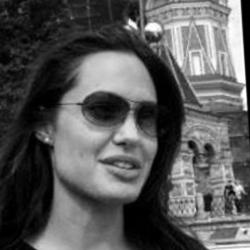
\includegraphics[width=\textwidth]{angelina/1}
        \end{subfigure}%
        ~ %add desired spacing between images, e. g. ~, \quad, \qquad etc.
        \begin{subfigure}[b]{0.2\textwidth}
                \centering
                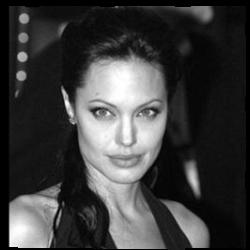
\includegraphics[width=\textwidth]{angelina/2}
        \end{subfigure}
        ~
        \begin{subfigure}[b]{0.2\textwidth}
                \centering
                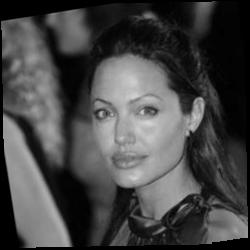
\includegraphics[width=\textwidth]{angelina/3}
        \end{subfigure}%
        ~ %add desired spacing between images, e. g. ~, \quad, \qquad etc.
        \begin{subfigure}[b]{0.2\textwidth}
                \centering
                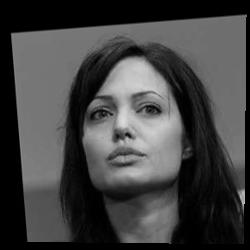
\includegraphics[width=\textwidth]{angelina/4}
        \end{subfigure}
%

        \begin{subfigure}[b]{0.2\textwidth}
                \centering
                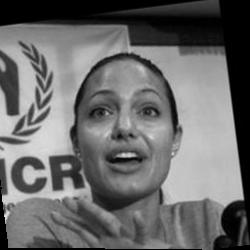
\includegraphics[width=\textwidth]{angelina/5}
        \end{subfigure}%
        ~ %add desired spacing between images, e. g. ~, \quad, \qquad etc.
        \begin{subfigure}[b]{0.2\textwidth}
                \centering
                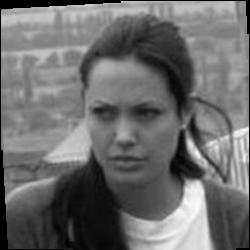
\includegraphics[width=\textwidth]{angelina/6}
        \end{subfigure}
        ~
        \begin{subfigure}[b]{0.2\textwidth}
                \centering
                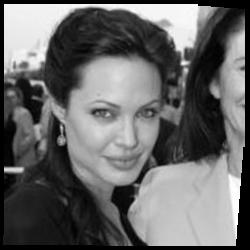
\includegraphics[width=\textwidth]{angelina/7}
        \end{subfigure}%
        ~ %add desired spacing between images, e. g. ~, \quad, \qquad etc.
        \begin{subfigure}[b]{0.2\textwidth}
                \centering
                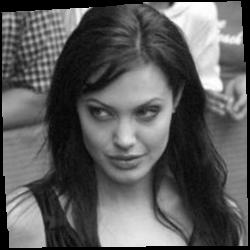
\includegraphics[width=\textwidth]{angelina/8}
        \end{subfigure}
%
        \begin{subfigure}[b]{0.2\textwidth}
                \centering
                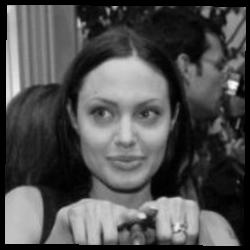
\includegraphics[width=\textwidth]{angelina/9}
        \end{subfigure}%
        ~ %add desired spacing between images, e. g. ~, \quad, \qquad etc.
        \begin{subfigure}[b]{0.2\textwidth}
                \centering
                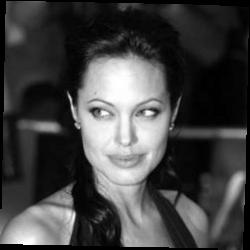
\includegraphics[width=\textwidth]{angelina/10}
        \end{subfigure}
        ~
        \begin{subfigure}[b]{0.2\textwidth}
                \centering
                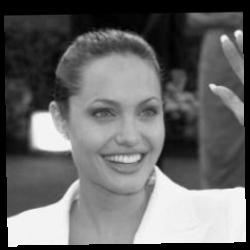
\includegraphics[width=\textwidth]{angelina/11}
        \end{subfigure}%
        ~ %add desired spacing between images, e. g. ~, \quad, \qquad etc.
        \begin{subfigure}[b]{0.2\textwidth}
                \centering
                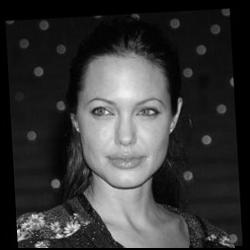
\includegraphics[width=\textwidth]{angelina/12}
        \end{subfigure}
%
        \begin{subfigure}[b]{0.2\textwidth}
                \centering
                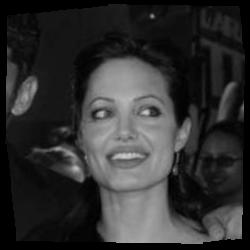
\includegraphics[width=\textwidth]{angelina/13}
        \end{subfigure}%
        ~ %add desired spacing between images, e. g. ~, \quad, \qquad etc.
        \begin{subfigure}[b]{0.2\textwidth}
                \centering
                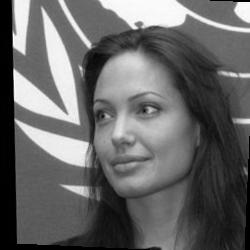
\includegraphics[width=\textwidth]{angelina/14}
        \end{subfigure}
        ~
        \begin{subfigure}[b]{0.2\textwidth}
                \centering
                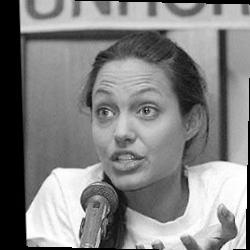
\includegraphics[width=\textwidth]{angelina/15}
        \end{subfigure}%
        ~ %add desired spacing between images, e. g. ~, \quad, \qquad etc.
        \begin{subfigure}[b]{0.2\textwidth}
                \centering
                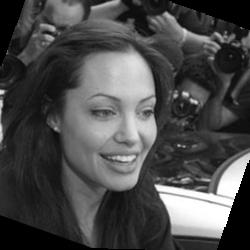
\includegraphics[width=\textwidth]{angelina/16}
        \end{subfigure}
        \caption{Exemplo de imagens do conjunto $\mathscr{G}$ para o sujeito Angelina Jolie}
        \label{fig:galeria}        
\end{figure}

A galeria de treino, $\mathscr{G}$, é constituída por 80\% das imagens de cada pessoa (16 imagens por pessoa), sendo as suas imagens utilizadas como amostras biométricas para o treino do sistema de reconhecimento facial. Um exemplo das imagens presentes na galeria de treino para o sujeito Angelina Jolie pode ser visto na figura \ref{fig:galeria}.

\begin{figure}
        \centering
        \begin{subfigure}[b]{0.2\textwidth}
                \centering
                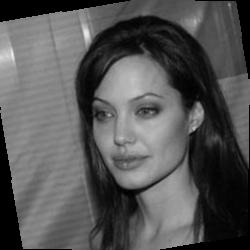
\includegraphics[width=\textwidth]{angelina/17}
        \end{subfigure}%
        ~ %add desired spacing between images, e. g. ~, \quad, \qquad etc.
        \begin{subfigure}[b]{0.2\textwidth}
                \centering
                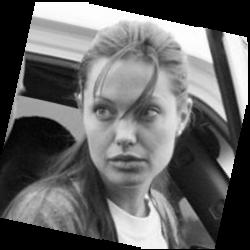
\includegraphics[width=\textwidth]{angelina/18}
        \end{subfigure}
        ~
        \begin{subfigure}[b]{0.2\textwidth}
                \centering
                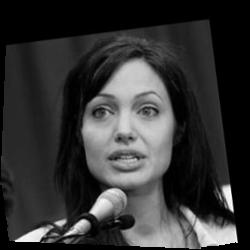
\includegraphics[width=\textwidth]{angelina/19}
        \end{subfigure}%
        ~ %add desired spacing between images, e. g. ~, \quad, \qquad etc.
        \begin{subfigure}[b]{0.2\textwidth}
                \centering
                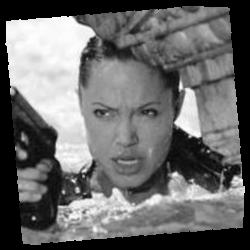
\includegraphics[width=\textwidth]{angelina/20}
        \end{subfigure}
        \caption{Exemplo de imagens do conjunto $\mathscr{P}$ para o sujeito Angelina Jolie}
        \label{fig:provas}   
\end{figure}

O conjunto $\mathscr{P}$ contem os restantes 20\% das imagens de cada pessoa (4 imagens por pessoa) e, tal como o seu nome indica, as suas imagens são utilizadas para a avaliação do sistema desenvolvido. Um exemplo das imagens presentes nas provas para o sujeito Angelina Jolie pode ser visto na figura \ref{fig:provas}.

A diferença existente entre os quatro conjuntos criados encontras-se relacionada com as imagens incluídas na galeria de treino e nas provas, sendo que estas diferem de forma aleatória entre os quatro conjuntos. A criação de 4 conjuntos com igual tamanho mas diferentes imagens de treino e teste tem em vista analisar o desempenho do sistema com diferentes galerias, de forma a determinar se existe uma variação significativa dos resultados obtidos em cada galeria.

\section{Pré-processamento} \label{sec:experiencias}
O módulo de reconhecimento facial, \textit{Face Recognizer}, disponibilizado pela plataforma \textit{OpenCV}, constituiu uma base sólida para o desenvolvimento do sistema de reconhecimento facial \textit{Visage}, contudo, de modo a tornar este sistema mais completo e versátil, revelou-se necessário adapta-lo e expandir as suas capacidades, nomeadamente através da aplicação de uma cadeia de pré-processamento às imagens existentes \footnote{a qual se encontra ilustrada na figura \ref{fig:preprocessamento}}. A evolução do sistema desenvolvido foi efetuada de forma gradual e iterativa, e culminou na construção de um conjunto de galerias de imagens, analisadas através de um grupo de experiências que permitem tirar conclusões acerca dos efeitos das diversas etapas de pré-processamento realizadas e da contribuição de cada uma delas para a melhoria do desempenho do sistema criado. 

Todas as galerias criadas possuem as imagens contidas nos conjuntos de teste definidos em \ref{sec:conjuntos}, diferenciando-se pelos diferentes passos de pré-processamento a que as imagens foram sujeitas. De notar que, tal  como representado em \ref{fig:preprocessamento}, o pré-processamento das imagens é efetuado antes da aplicação da máscara nas mesmas, de forma a não afetar os resultados obtidos nas tarefas de pré-processamento. Na tabela \ref{tab:colecoes} encontram-se resumidas as galerias resultantes do conjunto de experiências efetuadas, as quais se encontram descritas pormenorizadamente de seguida.

\subsection{Deteção e segmentação da face}
Na revisão efetuada ao estado da arte do reconhecimento facial em imagens destacou-se a importância da resolução de um conjunto de sub-problemas específicos para um reconhecimento facial eficaz (ver \ref{sec:sub-problemas}), nomeadamente a deteção e segmentação das faces existentes numa imagem. Para a resolução deste problema, foi implementado o módulo de deteção facial descrito em \ref{chap:facedetector}. Na implementação deste módulo revelou-se necessário a avaliação de diferentes alternativas relativamente à forma como é efetuada a segmentação da face da restante imagem, assim como a determinação do impacto dessa segmentação. 

Após uma análise das diferente alternativas existentes, e através de alguns teste intermédios realizados durante o período de desenvolvimento, foram então criadas as galerias de imagens Original, figura \ref{fig:original}; Cropped, figura \ref{fig:cropped}; e Masked, figura \ref{fig:masked}. A primeira, é constituída pelas imagens originais da biblioteca LFW-a e permite estabelecer uma base de comparação entre as imagens segmentadas e as imagens originais. A galeria cropped é composta por um conjunto de imagens onde as faces foram detetadas e segmentadas pelo detetor facial implementado e descrito no capítulo \ref{chap:facedetector}. A terceira e última galeria criada possui as mesmas imagens da galeria Cropped, sobre as quais foi posteriormente aplicada uma máscara elíptica de modo a diminuir a presença de fundo nas imagens recortadas.

\subsection{Normalização do Contraste}
A normalização das imagens em termos de contraste é passo comum e essencial à maioria dos sistemas de reconhecimento facial automático modernos, tal como destacado no capítulo \ref{chap:reco} desta dissertação. Assim sendo, no decorrer do desenvolvimento do sistema de reconhecimento facial Visage, revelou-se também importante analisar o qual o impacto da normalização do contraste nas imagens utilizadas, assim como qual a melhor forma de efetuar a sua normalização. Foram então estudadas três formas distintas de efetuar a normalização do contraste, as quais são apresentadas de seguida:

\begin{description}
\item[\textit{Contrast Streching}]
A técnica de \textit{Contrast Streching}, também designada por alguns autores simplesmente de normalização, consiste numa tentativa de alargar a gama de valores utilizados para codificar a intensidade de uma imagem de forma a que seja utilizada toda a gama de valores possíveis. Nesta avaliação as imagens utilizadas encontram-se convertidas para tons de cinzento, pelo que a normalização efetuada consiste num mapeamento linear dos valores originais para uma gama de intensidade entre 0 e 255. Da aplicação da técnica de contrast streching às imagens presentes nos conjuntos de teste descritos anteriormente resultou a criação da galeria Normalized. Um exemplo de uma imagem dessa galeria pode ser visualizado na imagem \ref{fig:normalized}.
\end{description}

\begin{description}
\item[Equalização Histograma]
O histograma de uma imagem descreve a distribuição estatística dos níveis de intensidade de uma imagem, neste caso concreto dos níveis de cinzento, em função do seu número de pixeis. A equalização do histograma de uma imagem consiste no mapeamento das variações da escala de cinzentos de forma a que o histograma resultante se aproxime de uma outra distribuição, mais alargada e idealmente uniforme na distribuição dos valores de intensidade da imagem. Este procedimento parte do princípio de que a qualidade da imagem é uniforme em toda a imagem, aplicando um mapeamento similar a toda a imagem \cite{Bradski2008}. As imagens normalizadas através da equalização simples do histograma encontram-se representadas na galeria Equalized e um exemplo das mesmas pode ser visto na figura \ref{fig:equalized}.
\end{description}

\begin{description}
\item[\textit{CLAHE}]
\textit{Contrast limited adaptive histogram equalization (CLAHE)} procura ultrapassar as limitações da equalização de contraste, através de uma abordagem local ao problema de normalização do histograma de uma imagem. Ao contrário da abordagem tradicional apresentada acima, esta técnica tem em conta a intensidade de um conjunto de pixeis e dos seus vizinhos para a normalização do seu contraste e não a intensidade de toda a imagem. Para além disso, tal como o seu nome indica, esta abordagem incluí ainda um limite para o qual a equalização do histograma é realizada, evitando assim a o mapeamento demasiado agressivo quando duas escalas de intensidade dispares se encontram na mesma região \cite{Reza2004}. Na imagem \ref{fig:clahe} encontra-se representada uma imagem da galeria CLAHE, resultante da normalização das imagens dos conjuntos de teste através da técnica CLAHE.
\end{description}

\subsection{Abstração Imagens}
A terceira experiência visa analisar o impacto da abstração de imagens no reconhecimento.

Gaussian Blur

Bilateral

Anisotropic Kuwahara

\begin{figure}
        \centering
        \begin{subfigure}[b]{0.2\textwidth}
                \centering
                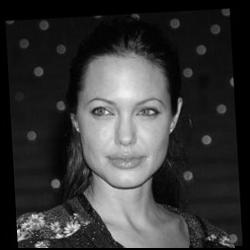
\includegraphics[width=\textwidth]{angelina/Angelina_Jolie_0006}
                \caption{Original}
                \label{fig:original} 
        \end{subfigure}%
%

        \begin{subfigure}[b]{0.2\textwidth}
                \centering
                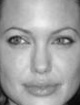
\includegraphics[width=\textwidth]{angelina/Angelina_Jolie_0006_cropped}
                \caption{Cropped}
                \label{fig:cropped} 
        \end{subfigure}
        ~ ~
        \begin{subfigure}[b]{0.2\textwidth}
                \centering
                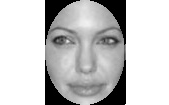
\includegraphics[width=\textwidth]{angelina/Angelina_Jolie_0006_masked}
                \caption{Masked}
                \label{fig:masked}
        \end{subfigure}%
%

        \begin{subfigure}[b]{0.2\textwidth}
                \centering
                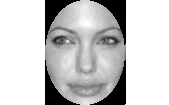
\includegraphics[width=\textwidth]{angelina/Angelina_Jolie_0006_normalized}
                \caption{Normalized}
                \label{fig:normalized} 
        \end{subfigure}
        ~ ~
        \begin{subfigure}[b]{0.2\textwidth}
                \centering
                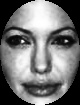
\includegraphics[width=\textwidth]{angelina/Angelina_Jolie_0006_equalized}
                \caption{Equalized}
                \label{fig:equalized}
        \end{subfigure}
        ~ ~
        \begin{subfigure}[b]{0.2\textwidth}
                \centering
                \includegraphics[width=\textwidth]{angelina/Angelina_Jolie_0006_CLAHE}
                \caption{CLAHE}
                \label{fig:clahe}
        \end{subfigure}
        \caption{Exemplo dos vários pré-processamentos disponíveis.}
        \label{fig:galeriaspreprocessadas}   
\end{figure}


\begin{center}
\begin{table}
	\caption{Galerias criadas após pré-processamento.}
	\begin{center}
    \begin{tabular}{l|cccc|c}
    \hline\hline
    Designação & Recortada   & Normalização           & Filtro Abstração & Máscara & Exemplo \\
	\hline
    Original   &   -         & -                      & -                &   -     & \ref{fig:original} \\
	~ & ~ & ~ & ~ & ~ & ~\\
    Cropped    & Sim         & -                      & -                &   -     & \ref{fig:cropped}  \\
    Masked     & Sim         & -                      & -                & Sim     & \ref{fig:masked}  \\
	~ & ~ & ~ & ~ & ~ & ~\\
    Normalized & Sim         & Constrast Streching    & -                & Sim     & \ref{fig:normalized}  \\
    Equalized  & Sim         & Histogram Equalization & -                & Sim     & \ref{fig:equalized}  \\
    CLAHE      & Sim         & CLAHE                  & -                & Sim     & \ref{fig:clahe}  \\
	~ & ~ & ~ & ~ & ~ & ~\\
    Bilateral  & Sim         & Histogram Equalization & Bilateral Filter & Sim       \\
    Gaussian   & Sim         & Histogram Equalization & Gaussian Filter  & Sim       \\
    \hline\hline
    \end{tabular}
	\label{tab:colecoes}
	\end{center}
\end{table}
\end{center}


\section{Avaliação \textit{Closed-Set Identification}} \label{sec:avaliacao1}
Tal como introduzido na secção \ref{sec:problema}, o paradigma de \textit{closed-set identification}, constitui um sub-problema de identificação em que uma prova é apresentada ao sistema e pretende-se que este devolva a identidade da pessoa presente na imagem. Neste caso particular do problema de identificação, todas as provas apresentadas possuem uma correspondência na galeria, em oposição ao caso geral de identificação, no qual pode ou não haver uma correspondência.

A avaliação \textit{closed-set} é uma medida padrão de avaliação do desempenho em sistemas de reconhecimento facial automático, tendo sido utilizada em diversas avaliações efetuadas, nomeadamente nas avaliações FERET e FRVT apresentadas na revisão do estado da arte desta dissertação (ver \ref{chap:reco}). A utilização de um conjunto fechado de imagens permite uma análise detalhada do desempenho de um algoritmo permitindo responder à pergunta "a identificação correta encontra-se nos primeiros $n$ resultados?" em vez de apenas " o primeiro resultado é o correto?".

\subsection{Metodologia Avaliação}
Para cada conjunto de teste descrito em \ref{sec:conjuntos}, seja $\mathscr{G}$ a sua galeria de treino, em que $\mathscr{G} = \{g_1, ..., g_N\}$ e seja $\mathscr{P}$ o conjunto das suas provas, em que $\mathscr{P} = \{p_1, ..., p_N\}$. Quando uma prova $p_j$ é apresentada ao sistema, essa prova é então comparada a cada amostra biométrica $g_i$ da galeria, resultando dessa comparação o respetivo índice de similaridade (\textit{similarity score}), $s_{ij}$. Este índice é designado de $match$ $score$, caso $g_i$ e $p_j$ sejam amostras da mesma pessoa, caso não o sejam é designado de $nonmatch$ $score$. Quanto menor o índice de similaridade, maior é a probabilidade das imagens comparadas pertencerem à mesma pessoa, sendo que o melhor valor possível para o índice de similaridade de um $match$ $score$ é zero.

Na identificação de $p_j \in \mathscr{P}$, em primeiro lugar são calculados os índices de similaridade para todas as amostras na galeria $\mathscr{G}$, sendo posteriormente ordenados os seus resultados. O ranking de $p_j$, $r_{p_j}$, é igual a $n$, se o seu $match$ $score$ corresponde ao enésimo menor índice de similaridade. A taxa de identificação para o ranking $n$, $T_{I}(n)$, corresponde à fração de provas com ranking $n$ ou menor do que $n$, ou seja:
\begin{equation}
T_{I}(n) = \frac{|C(n)|}{|\mathscr{P}|} \times 100
\end{equation}
Em que $|C(n)|$ é número de provas com ranking $n$, ou menor do que $n$, e $|\mathscr{P}|$ o número de provas existentes em $\mathscr{P}$.

A $T_{I}(n)$ é calculada para todos os rankings entre 1 e 30. Dentro desse intervalo, os primeiros níveis de ranking apresentam uma maior variação na percentagem de pessoas identificadas, revelando-se assim mais significativos para a análise do desempenho do sistema.

A avaliação é efetuada através da análise do desempenho dos três algoritmos disponíveis em cada uma das galerias de imagens pré-processadas, encontrando-se os resultados obtidos agrupados num conjunto de três experiências, cada uma dedicada a analisar a variação do comportamento do sistema dado um problema específico. A divisão entre imagens de treino e teste de cada galeria é efetuada segundo os quatro conjuntos de testes criados, sendo cada galeria avaliada em cada um dos quatro conjuntos de teste existentes e posteriormente calculada a média dos resultados obtidos.

A média dos resultados obtidos encontra-se representada em um gráfico do tipo \textit{Cumulative match score} (CMS). Um gráfico do tipo CMS representa $T_{I}(n)$ como uma função de ranking $n$. No eixo horizontal encontra-se representado o ranking e no eixo vertical encontra-se representada a respetiva taxa de identificação, um exemplo de um gráfico CMS pode ser visto em \ref{fig:exp1_comaparacao}.

\subsection{Resultados Experiência 1 : Análise do impacto da segmentação das faces}

\begin{figure}[p]
        \centering
        \begin{subfigure}[b]{0.58\textwidth}
                \centering
                \includegraphics[width=\textwidth]{resultados/original_cropped_masked_eigen}
                \caption{Eigenfaces}
                \label{fig:original_cropped_masked_eigen}
        \end{subfigure}%

        \begin{subfigure}[b]{0.58\textwidth}
                \centering
                \includegraphics[width=\textwidth]{resultados/original_cropped_masked_fisher}
                \caption{Fisherfaces}
                \label{fig:original_cropped_masked_fisher}
        \end{subfigure}

        \begin{subfigure}[b]{0.58\textwidth}
                \centering
                \includegraphics[width=\textwidth]{resultados/original_cropped_masked_lbph}
                \caption{LBPH}
                \label{fig:original_cropped_masked_lbph}
        \end{subfigure}
        \caption{Desempenho algoritmos Eigenfaces, Fisherfaces e LBPH para os conjuntos Original, Cropped e Masked}
        \label{fig:original_cropped_masked}
\end{figure}

Esta experiência visa analisar o impacto da segmentação das faces presentes na imagem do fundo existente nas mesmas, assim como determinar qual, de entre duas alternativas, a melhor forma de segmentar essa mesma face. Os resultados obtidos podem ser visualizados na figura \ref{fig:original_cropped_masked}, onde se encontram ilustrada a performance dos algoritmos, \textit{Eigenfaces}, \textit{Fisherfaces} e \textit{LBPH}, nos três conjuntos criados especialmente para esta experiência, os quais se encontram descritos mais pormenorizadamente em \ref{sec:experiencias}.

Após a analise dos resultados obtidos na experiência 1, nomeadamente através da comparação das taxa de identificação de ranking 1 dos conjuntos Cropped e Masked com o conjunto Original, verifica-se que a segmentação das faces presentes nas imagens originais produz uma melhoria efetiva dos resultados obtidos, traduzindo-se num aumento de cerca de 12\%, 14\% e 40\% para os algoritmos \textit{Eigenfaces}, \textit{Fisherfaces} e \textit{LBPH}, respetivamente.

Uma análise mais aprofundada desses resultados, demonstra ainda que, no caso dos algoritmos \textit{Eigenfaces} e \textit{LBPH}, a diferença na taxa de identificação entre as imagens originais (conjunto Original) e as imagens segmentadas (conjuntos Cropped e Masked) é significativa e relativamente constante nos vários níveis para os quais a taxa de deteção se encontra reportada. Por outro lado, no caso do algoritmo \textit{Fisherfaces}, apesar da diferença significativa no número de imagens corretamente identificadas nos primeiros níveis, a partir do ranking 15, todos os conjuntos de imagens obtém uma taxa de identificação similar, e com uma progressão semelhante. Esta aproximação no número de caras corretamente identificadas nos rankings mais elevados pode ser explicada pela existência de informação no fundo das imagens, a qual poderá ser utilizada pelo próprio algoritmo para a identificação das mesmas, ao invés da utilização da face contida na imagem, reforçando assim a importância da extração do fundo contido nas imagens originais.

Por outro lado, note-se ainda que, apesar do impacto positivo da segmentação das imagens nos três algoritmos testados, o impacto desta segmentação varia significativamente conforme o algoritmo utilizado, sendo que o \textit{Fisherfaces} é o que revela resultados mais constantes independentemente da manipulação efetuada nas imagens e o algoritmo \textit{LBPH} o que regista uma maior melhoria desses mesmos resultados.

Ao nível da diferença entre as imagens apenas segmentadas (conjunto Cropped) e as imagens com máscara (conjunto Masked), é possível verificar que ambas possuem resultados semelhantes, sendo que a maior diferença foi detetada no algoritmo \textit{Eigenfaces}, onde as imagens com máscara demonstraram um desempenho ligeiramente superior, como é possível verificar pelas $T_{I}(2)$ de 43,4\% e 40,1\% para as imagens com máscara e recortadas, respetivamente. Apesar da diferença registada ser muito significativa, a existência de uma máscara garante uma extração de uma maior quantidade de fundo das imagens, permitindo assim uma maior confiança dos resultados obtidos, no sentido em que se reduz o perigo de identificação pelas características do fundo da imagem e não das caraterísticas faciais presentes na mesma. 

\begin{figure}[ht]
  \begin{center}
    \leavevmode
    \includegraphics[width=0.6\textwidth]{resultados/exp1_comparacao}
    \caption{Comparação do desempenho dos três algoritmos implementados para o conjunto Masked}
    \label{fig:exp1_comaparacao}
  \end{center}
\end{figure}

Finalmente, através da análise do gráfico \ref{fig:exp1_comaparacao}, é possível concluir que ao nível dos algoritmos utilizados o algoritmo \textit{LBPH} obtém resultados globalmente melhores, ao passo que o algoritmo \textit{Eingefaces} obtém os piores resultados. Esta diferença verifica-se quer nos rankings inferiores, quer nos superiores, sendo menor quanto maior é o ranking utilizado, como é possível verificar pelas taxas de identificação de ranking 1 de 46,8\% e 28,1\%, no conjunto Masked, para os algoritmos \textit{LBPH} e \textit{Eigenfaces}, respetivamente, e pelas taxas de identificação de ranking 30 de 94,9\% e 89,3\%, para os mesmos algoritmos no mesmo conjunto.

\subsection{Resultados Experiência 2: Impacto da Normalização do Contraste}
\begin{figure}[p]
        \centering
        \begin{subfigure}[b]{0.58\textwidth}
                \centering
                \includegraphics[width=\textwidth]{resultados/Exp_2_eigen}
                \caption{Eigenfaces}
                \label{fig:masked_normalized_equalized_clahe_eigen}
        \end{subfigure}%

        \begin{subfigure}[b]{0.58\textwidth}
                \centering
                \includegraphics[width=\textwidth]{resultados/Exp_2_fisher}
                \caption{Fisherfaces}
                \label{fig:masked_normalized_equalized_clahe_fisher}
        \end{subfigure}

        \begin{subfigure}[b]{0.58\textwidth}
                \centering
                \includegraphics[width=\textwidth]{resultados/Exp_2_lbph}
                \caption{LBPH}
                \label{fig:masked_normalized_equalized_clahe_lbph}
        \end{subfigure}
        \caption{Desempenho algoritmos Eigenfaces, Fisherfaces e LBPH para os conjuntos Normalized, Equalized e CLAHE}
        \label{fig:exp2}
\end{figure}

A aquisição de imagens em condições não controladas pode resultar na obtenção de fotografias com um contraste reduzido e níveis de iluminação muito distintos. De forma a ultrapassar este problema, a normalização do contraste de uma imagem é uma tarefa comum nos sistemas de reconhecimento faciais modernos. Nesta experiência pretendemos analisar qual o impacto da normalização do contraste de uma imagem nos diferentes algoritmos implementados, assim como determinar qual a melhor de entre três técnicas distintas implementadas, através da analise do desempenho do sistema em três galerias previamente normalizadas com cada uma dessas técnicas (ver \ref{sec:experiencias}).

Na figura \ref{fig:exp2} é possível visualizar os resultados para obtidos para o desempenho do sistema nas galerias Normalized, Equalized e CLAHE, correspondentes às três técnicas de normalização \textit{contrast stretching}, equalização histograma e CLAHE, respectivamente. Nos gráficos da figura \ref{fig:exp2} encontra-se ainda representados os resultados obtidos para o conjunto Masked, utilizado na experiência 1, o qual serve de referência para a comparação entre os conjuntos não normalizados e os conjuntos normalizados.

Como é possível concluir pela observação da figura \ref{fig:exp2}, a normalização das imagens apresenta resultados globalmente melhores do que os obtidos para conjuntos não normalizados. O impacto obtido varia, no entanto, consideravelmente conforme o algoritmo utilizado, sendo que o maior impacto é registado para o algoritmo Eigenfaces, onde existe uma melhoria na ordem dos 15.0\% na percentagem de pessoas reconhecidas no primeiro nível do ranking, quando comparadas as galerias Masked e Equalized. Os algoritmos \textit{Fisherfaces} e \textit{LBPH} mostram uma diferença máxima de apenas 3.8\% e 2.2\% entre os conjuntos Masked e Equalized, pelo que é possível concluir que estes algoritmos possuem uma maior resistência aos efeitos da iluminação no desempenho quando comparados com o algoritmo \textit{Eigenfaces} \footnote{A pouca variação obtida neste dois últimos algoritmos vai de acordo com o defendido por investigações anteriores realizadas por \cite{ahonen2004face}.}.

Ao nível das três técnicas utilizadas é possível concluir que as duas variantes de equalização do histograma possuem os resultados mais satisfatórios. A equalização simples do histograma, conjunto Equalized, tem tendência a demonstrar resultados melhores para os primeiros níveis de ranking, sendo posteriormente igualada ou até ultrapassada pela técnica CLAHE nos níveis mais superiores. Uma vez que os primeiros níveis de ranking incluem a informação mais significativa para a maioria dos utilizadores de sistemas de reconhecimento facial automático, consideramos que o desempenho da equalização do histograma das imagens possuí resultados mais relevantes para a utilização no sistema de reconhecimento facial Visage do que a técnica \textit{CLAHE}.

\begin{figure}[ht]
  \begin{center}
    \leavevmode
    \includegraphics[width=0.6\textwidth]{resultados/exp2_comparacao}
    \caption{Comparação do desempenho dos três algoritmos implementados para o conjunto Equalized}
    \label{fig:exp2_comaparacao}
  \end{center}
\end{figure}

Finalmente, a análise comparativa dos resultados obtidos para os três algoritmos implementados, ilustrada pelo gráfico \ref{fig:exp2_comaparacao}, permite concluir que após a normalização do histograma das imagens o desempenho dos algoritmos apresenta uma diferença muito menor do que a registada anteriormente e ilustrada pelo gráfico \ref{fig:exp1_comaparacao}. Nesta experiência o algoritmo LBPH continua a ser o algoritmo com melhor desempenho, registando no entanto uma diferença de apenas 1.8\% e 6.0\% para os algoritmos \textit{Fisherfaces} e \textit{Eigenfaces}, respetivamente, na taxa de identificação de ranking 1 no conjunto Equalized. De notar ainda que, a partir do segundo nível do ranking, o algoritmo  \textit{Eigenfaces} possui uma taxa de identificação idêntica ao valores obtidos pela algoritmo \textit{Fisherfaces}, ultrapassando o desempenho do segundo, a partir do ranking 11. Esta grange evolução no desempenho, notada para o algoritmo \textit{Eigenfaces}, em contraste com a ligeira melhoria obtida pelos restantes denota a complexidade associada ao problema de reconhecimento facial automático, nomeadamente no que diz respeito à forma como diferentes fatores afetam de forma diferenciada diferentes algoritmos e diferentes conjuntos de dados.

\subsection{Resultados Experiência 3}

\section{Avaliação \textit{Image Retrieval}} \label{sec:avaliacao2}
A metodologia de avaliação proposta na secção \ref{sec:avaliacao1} desta dissertação permite-nos efetuar uma avaliação qualitativa do desempenho do sistema de reconhecimento facial criado, assim como dos diferentes algoritmos implementados, através de uma medida padrão para a avaliação de sistemas de reconhecimento facial automáticos. Nesta segunda avaliação propomos a avaliação do desempenho do sistema de um ponto de vista centrado num possível caso de uso do mesmo: \textit{Image Retrieval}.

A área de recuperação de informação multimédia regista atualmente uma importância crescente, resultado do elevado número de conteúdos produzidos, assim como do elevado número de dispositivos de partilha disponíveis, tal como destacado no estado da arte desta dissertação. Desta forma, a recuperação de informação multimédia e em particular a área de \textit{Image Retrieval} representa uma das áreas com maior potencial para a utilização do sistema de reconhecimento facial criado.

Para uma dada imagem contendo uma face, o sistema Visage é capaz de detetar a face presente na imagem e apresentar uma lista ordenada de possíveis entidades que se encontram representadas nessa imagem. Com base neste sistema é possível desenvolver aplicações de \textit{image retrieval} capazes de encontrar fotos de uma personalidade específica ou apresentar, para uma foto de rosto fornecida pelo utilizador, a celebridade ou figura pública mais parecida.

\subsection{Metodologia Avaliação}
Em recuperação de informação multimédia designa-se de \textit{precisão} a fração de documentos relevantes do total de documentos retornados por uma pesquisa. Ao analisar a precisão podem ser analisados todos os documentos relevantes ou apenas os $n$ documentos mais relevantes, designado-se nessa situação de \textit{precisão a n}.

No sistema de reconhecimento facial criado, para uma dada imagem é apresentada uma lista de possíveis entidades que se encontram representadas nessa imagem, em que o primeiro resultado representa a entidade com maior probabilidade de estar presente na imagem e em que cada entidade aparece uma única vez na lista de resultados possíveis. Caso se pretenda efetuar a identificação de uma personalidade existe apenas um resultado verdadeiramente relevante na lista de resultados obtida, pelo que a medida de \textit{precisão a n} utilizada em recuperação de informação multimédia não é válida para a avaliação efetuada nesta secção.

Para avaliação do desempenho do sistema do ponto de vista de \textit{image retrieval} foi então criada a medida \textit{precisão na galeria} (PG). A \textit{precisão na galeria} resulta da adaptação da precisão de recuperação de informação multimédia ao caso particular do sistema de reconhecimento facial automático desenvolvido. Considerando a definição de ranking de uma prova apresentada em \ref{sec:avaliacao1}, a \textit{precisão na galeria} de $p_j$, $PG_{p_j}$, corresponde a:

\begin{equation}
PG_{p_j} = \frac{1}{r_{p_j}} \times 100
\end{equation}

Em que $\mathscr{P}$ é o conjunto de provas da galeria, $p_j \in \mathscr{P}$ e $r_{p_j}$ corresponde ao ranking da prova $p_j$.

A \textit{precisão na galeria} de uma prova progride então de 100\% para ranking 1, 50\% para ranking 2, 33\% ranking 3 e assim sucessivamente. As provas com um menor ranking têm então uma maior precisão, assim como uma maior distância entre si em termos de precisão (50 unidades entre 1 e 2, 22 unidades entre 2 e 3, etc). Ora, no caso de \textit{image retrieval} é importante que o resultado mais relevante, a identificação correta de uma pessoa, surja com o menor ranking possível, pelo que a distância nas \textit{precisões na galeria} obtidas nos primeiros resultados deve ser maior do que a obtida para os resultados que surgem posteriormente na lista de entidades possíveis, tal como verificado na métrica adotada. Desta forma, é possível analisar a desempenho do sistema com ênfase nos resultados de topo para uma determinada prova, beneficiando os valores de \textit{precisão na galeria} quando o nome correto aparece cedo na lista de resultado possíveis, ao mesmo tempo que se diferencia significativamente os resultados de topo.

Dada a \textit{precisão na galeria} a \textit{média da precisão na galeria} (MPG) de um algoritmo é calculada através da média da \textit{precisão na galeria} obtida para cada prova, ou seja:
\begin{equation}
MPG_{algoritmo} = \frac{ \sum\limits_{i=0}^{n} PG_{p_i} }{n}
\end{equation}

Em que $n$ corresponde ao número de provas existentes em $\mathscr{P}$.

\subsection{Resultados}
Na tabela \ref{tab:resultadosprecicao} encontram-se representada a média dos resultados obtidos nos quatro conjuntos de teste existentes para a\textit{média da precisão na galeria} dos três algoritmos implementados em cada uma das galerias introduzidas em \ref{sec:experiencias}.

-LBPH tem maior precisão em todos os conjuntos à excepção das imagens não manipuladas.

-Conjuntos Cropped e Masked tem resultados semelhantes.

-Má manipulação pode reduzir eficácia, exemplo Normalized.

-Equalized é o que apresenta melhores resultados para os três algoritmos

-Corte e Equalização reduzem as diferenças de desempenho entre os algoritmos.

\begin{center}
\begin{table}
    \begin{center}
    \caption{Resultados Média Precisão na Galeria (melhores a negrito)}
    \begin{tabular}{l|ccc}
    Galeria    & $MPG_{Eigenfaces}$ & $MPG_{Fisherfaces}$ & $MPG_{LBPH}$ \\ 
    \hline\hline
    Original   & 23.1\%          & \textbf{43.4\%}  & 16.0\%             \\
    ~ \\
    Cropped    & 37.7\%          & 54.8\%           & \textbf{58.2\%}    \\
    Masked     & 40.0\%          & 54.0\%           & \textbf{58.3\%}    \\
    ~ \\
    Normalized & 42.4\%          & 53.5\%           & \textbf{57.2\%}    \\
    Equalized  & 55.2\%          & 57.3\%           & \textbf{59.6\%}    \\
    CLAHE      & 53.6\%          & 55.9\%           & \textbf{56.5\%}    \\
    \hline\hline
    \end{tabular}
    \label{tab:resultadosprecicao}
    \end{center}
\end{table}
\end{center}


\section{Variação Desempenho} \label{sec:variacaodesempenho}
Considerando que de um ponto de vista estatístico um algoritmo de reconhecimento facial estima a identidade de uma face, é então possível interrogarmos-nos se, para uma dada categoria de imagens, se verifica uma variação no desempenho de um algoritmo quando são utilizadas galerias de treino e provas diferentes \cite{Phillips2000}.

Para o estudo do desempenho do sistema de reconhecimento facial Visage foram criados quatro conjuntos de teste, que designamos aqui de A, B, C, D, onde a diferença entre os quatro conjuntos se encontra nas imagens utilizadas como galeria de treino e provas, tal com descrito em \ref{sec:conjuntos}. As imagens de cada conjunto podem ser sujeitas a um conjunto de operações de pré-processamento diferentes, resultantes na criação das galerias original, cropped, masked, normalized, equalized e CLAHE, onde cada galeria contem todas as imagens dos quatro conjuntos de teste, tal como descrito em \ref{sec:experiencias}.

Nesta secção é efetuada a análise do desempenho do sistema nos quatro conjuntos de teste criados em cada uma das galerias existente.

-Conjunto B obtém melhor desempenho em todos os algoritmos e todas as galerias.

-No conjunto B Fisherfaces obtem melhores resultados

-LBPH é o que apresenta melhor desempenho e menor desvio padrão

\begin{center}
\begin{table}
    \begin{center}
    \caption{Algoritmos ordenados por desempenho nos diversos conjuntos de teste, em cada galeria (L = LBPH, F = Fisherfaces, E = Eigenfaces).}
    \begin{tabular}{l|cccc}
    Galeria    & A & B & C & D \\ 
    \hline\hline
    Original   & F, E, L          &\textbf{ F, E, L }         & F, E, L           & F, E, L    \\
    ~ \\
    Cropped    & L, F, E          & L, F, E          & L, F, E           & L, F, E    \\
    Masked     & L, F, E          & L, F, E          & L, F, E           & L, F, E    \\
    ~ \\
    Normalized & L, F, E          &\textbf{ F, L, E}          & L, F, E           & L, F, E    \\
    Equalized  & L, F, E          &\textbf{ F, L, E}          & L, F, E           & L, F, E    \\
    CLAHE      & L, F, E          &\textbf{ F, L, E}          & L, F, E           & L, F, E    \\
    \hline\hline
    \end{tabular}
    \label{tab:ordem_algoritmos}
    \end{center}
\end{table}
\end{center}

\begin{center}
\begin{table}
    \begin{center}
    \caption{Desvio padrão ($\sigma$) entre os valores de MPG obtidos para os 4 conjuntos de teste.}
    \begin{tabular}{l|ccc}
    Galeria    & $\sigma_{Eigenfaces}$ & $\sigma_{Fisherfaces}$ & $\sigma_{LBPH}$ \\ 
    \hline\hline
    Original   & 1.21\%          & 1.12\%           & \textbf{0.39\%}    \\
    ~ \\
    Cropped    & 2.44\%          & 2.41\%           & \textbf{1.91\%}    \\
    Masked     & 2.83\%          & 3.29\%           & \textbf{1.46\%}    \\
    ~ \\
    Normalized & 2.09\%          & 3.85\%           & \textbf{1.36\%}    \\
    Equalized  &\textbf{ 1.13\%} & 2.26\%           & \textbf{1.13\%}    \\
    CLAHE      & 2.38\%          & 4.03\%           & \textbf{1.17\%}    \\
    \hline\hline
    \end{tabular}
    \label{tab:desviopadrao}
    \end{center}
\end{table}
\end{center}

\section{Discussão Resultados Obtidos} \label{sec:discussao}

\chapter{Conclusões e Perspetivas Futuras} \label{chap:conclusao}

\section{Conclusões}
A investigação realizada no âmbito desta dissertação teve como principal objetivo estudar o impacto do uso da abstração de imagens no processo de reconhecimento facial automático, assim como de um conjunto de tarefas de pré-processamento efetuadas sobre as imagens. Tendo em vista esse objetivo, foi desenvolvido o sistema de reconhecimento facial Visage. Para uma dada imagem fornecida ao sistema Visage, é aplicada sobre ela uma cadeia de pré-processamento, na qual a abstração de imagens se encontra incluída, e é efetuado posteriormente o seu reconhecimento, sendo devolvida uma lista ordenada de possíveis entidades contidas na imagem original.

Através da análise do estado da arte apresentada é possível concluir que o reconhecimento facial em imagens é um tema atual e onde se tem verificado um interesse crescente devido às suas múltiplas áreas de aplicação, assim como ao elevado valor comercial tradicionalmente associado a este tipo de soluções. 

O problema de reconhecimento facial é, no entanto, um problema complexo que integra, também ele, um conjunto de sub-problemas  complexos. Estes sub-problemas, aliados as múltiplas áreas de aplicação do reconhecimento facial, fazem com que exista uma grande variação do desempenho dos sistemas existentes, a qual se encontra diretamente relacionada com as condições de utilização dos mesmos, nomeadamente ao no que diz respeito às galerias de imagens utilizadas. A este nível, em situações onde as condições de captura das imagens são controladas e existe uma cooperação ativa por parte dos utilizadores os resultados obtidos são muito satisfatórios, sendo mesmo considerado que, nestas situações, o problema se encontra praticamente resolvido. Em contraste, em situações de captura não controladas e onde exista uma variação da iluminação, pose e expressão dos indivíduos este é ainda um problema desafiante e onde se verifica necessidade de investigação na atualidade.

Por outro lado, os filtros de abstração são ferramentas computacionalmente eficazes de abstração de informação, sendo tradicionalmente utilizados para comunicar mais eficazmente uma mensagem visual. Para além disso, o uso destes filtros para a pesquisa baseada em conteúdos com vista a ilustração automática de texto demonstrou resultados positivos quer ao nível da informação retornada, quer ao nível das necessidades de armazenamento das imagens.

Tendo em conta a pertinência do estudo no âmbito do reconhecimento facial automático em situações de captura de imagens não controladas, assim como a inexistência de estudos relativos ao impacto da utilização de filtros de abstração no processo de reconhecimento, a investigação levada a cabo no âmbito desta dissertação contribui de forma relevante para o conhecimento existente na área. 

Ao nível das avaliações efetuadas, é possível concluir que a deteção e segmentação correta das faces constituem as etapas de pré-processamento mais relevantes para a obtenção de resultados positivos no reconhecimento dos indivíduos, independentemente do algoritmo de reconhecimento utilizado. Por outro lado, a normalização do contraste das imagens através da equalização do seu histograma revela uma melhoria significativa nos resultados obtidos com particular ênfase no algoritmo \textit{Eigenfaces}. 

Finalmente, a integração da abstração de imagens no processo de reconhecimento apresenta um compromisso entre a diminuição da necessidade de processamento e armazenamento necessárias, com a ligeira diminuição da eficácia do reconhecimento. A este nível destaca-se o filtro Kuwahara anisotrópico, o qual representa o maior grau de abstração dos filtros utilizados, permitindo uma diminuição considerável do tamanho da galeria processada, mas que regista também um maior impacto no desempenho do reconhecimento.

Por último, a implementação do sistema Visage com base em uma biblioteca de código aberto permite também alargar o número de soluções atualmente existentes a este nível, ao mesmo tempo que constitui uma base sólida para o desenvolvimento de futuras aplicações que tirem partido do reconhecimento facial automático em imagens no seu funcionamento.

\section{Perspetivas Futuras}
O sistema de reconhecimento facial desenvolvido, assim como as avaliações efetuadas, vão de encontro aos objetivos traçados no âmbito desta dissertação, permitindo contribuir ativamente para o conhecimento existente acerca da aplicação de filtros de abstração no processo de reconhecimento facial em imagens. De seguida, encontra-se resumido algum do trabalho futuro com vista a melhorar o sistema de reconhecimento facial Visage, assim como expandir as conclusões da avaliação efetuada.

A primeira etapa de pré-processamento aplicada no sistema Visage corresponde à deteção das faces presentes numa imagem. Nesta fase, é apenas considerada a existência de uma cara relevante na imagem e é utilizado um classificador em cascata treinado para caras em posição frontal. A expansão desta etapa de pré-processamento, permitindo a identificação de múltiplas pessoas na mesma imagem, seria um próximo passo na melhoria da etapa de deteção facial. A utilização de vários classificadores diferentes correspondentes às múltiplas poses representadas nas diferentes imagens permitiria também efetuar uma deteção facial mais robusta, para além de possibilitar a criação de modelos de reconhecimento facial focados em reconhecer imagens de uma pessoa com uma pose específica.

Ao nível das restantes tarefas de pré-processamento aplicadas antes de efetuar a abstração das imagens existe também algum espaço para melhoria. Em primeiro lugar, o processo de alinhamento das imagens poderia ser melhorado de forma a o tornar mais robusto e ter em consideração a pose de uma face no seu alinhamento. No que diz respeito às técnicas de normalização do contraste, a diferença obtida com recurso à equalização do histograma e com recurso à técnica \textit{CLAHE} indicam também que esta é uma área onde existe um espaço para melhoria.

A abstração de imagens foi efetuada com recurso a três filtros distintos, os quais representam três graus de abstração de complexidade diferente. No âmbito de trabalho futuro a avaliação de outras técnicas de abstração de imagens poderá ser considerada.

A arquitetura do sistema Visage baseou-se na implementação de múltiplas aplicações do tipo caixa preta, onde para um conjunto de dados de entrada é produzido um resultado específico, sem que para isso seja necessário ter um conhecimento aprofundado acerca do funcionamento do sistema. A integração e eventual adaptação deste sistema a uma arquitetura cliente-servidor poderia permitir uma utilização dos métodos implementados de uma forma mais simples e intuitiva por parte de outras aplicações.


 

%% Comment next 2 commands if numbered appendices are not used
%%\appendix
%%\chapter{Avaliação \textit{Closed-set Identification}} \label{ap1:closed-set}
Nas tabelas abaixo encontram-se representados os resultados obtidos na avaliação \textit{Closed-set Identification}, para as nove galerias avaliadas, agrupados pelo algoritmo utilizado.

\begin{table}[h]
    \begin{center}
    \caption{Média dos resultados obtidos para o algoritmo \textit{Eigenfaces} nos 4 conjuntos de teste avaliados.}	
	\begin{tabular}{c|p{1.2cm}p{1.1cm}p{1.1cm}p{1.7cm}p{1.5cm}p{1.2cm}p{1.2cm}p{1.2cm}p{1.2cm}}
	Rank & Original & Cropped & Masked & Normalized & Equalized & CLAHE & Gaussian & Bilateral & AKF \\ 
	\hline\hline
	1 & 12.9\% & 25.9\% & 28.1\% & 30.0\% & 43.0\% & 40.9\% & 43.4\% & 42.7\% & 41.0\% \\ 
	2 & 18.3\% & 34.3\% & 37.7\% & 39.1\% & 55.3\% & 52.5\% & 55.5\% & 54.1\% & 51.5\% \\ 
	3 & 23.8\% & 40.2\% & 43.4\% & 45.9\% & 60.7\% & 59.8\% & 61.2\% & 60.7\% & 58.9\% \\ 
	4 & 27.9\% & 46.3\% & 47.9\% & 52.1\% & 64.6\% & 64.1\% & 65.3\% & 64.3\% & 62.5\% \\ 
	5 & 31.9\% & 50.0\% & 52.8\% & 56.7\% & 68.3\% & 68.0\% & 68.5\% & 67.9\% & 66.1\% \\ 
	6 & 35.7\% & 53.8\% & 55.7\% & 60.3\% & 70.8\% & 71.4\% & 71.7\% & 70.8\% & 69.5\% \\ 
	7 & 39.4\% & 57.0\% & 58.3\% & 62.9\% & 73.1\% & 73.6\% & 73.5\% & 72.9\% & 72.0\% \\ 
	8 & 41.3\% & 60.1\% & 61.1\% & 65.7\% & 74.6\% & 75.6\% & 75.5\% & 74.8\% & 73.6\% \\ 
	9 & 44.8\% & 62.2\% & 63.9\% & 68.6\% & 76.1\% & 78.0\% & 76.5\% & 76.2\% & 75.4\% \\ 
	10 & 47.6\% & 64.0\% & 65.8\% & 70.4\% & 77.9\% & 80.3\% & 78.3\% & 77.7\% & 76.4\% \\ 
	11 & 49.4\% & 66.1\% & 68.3\% & 72.7\% & 80.1\% & 81.4\% & 79.9\% & 79.0\% & 78.0\% \\ 
	12 & 51.9\% & 68.6\% & 70.2\% & 73.9\% & 81.4\% & 82.6\% & 81.4\% & 80.8\% & 79.7\% \\ 
	13 & 53.8\% & 70.8\% & 71.5\% & 75.5\% & 82.6\% & 84.2\% & 82.3\% & 81.9\% & 80.9\% \\ 
	14 & 55.7\% & 71.8\% & 73.1\% & 76.9\% & 83.6\% & 85.3\% & 84.0\% & 84.0\% & 82.5\% \\ 
	15 & 57.7\% & 72.9\% & 75.0\% & 79.7\% & 84.3\% & 86.8\% & 85.0\% & 85.1\% & 83.4\% \\ 
	16 & 59.8\% & 75.2\% & 77.0\% & 80.8\% & 85.6\% & 87.6\% & 85.9\% & 85.7\% & 84.5\% \\ 
	17 & 60.9\% & 76.9\% & 78.2\% & 81.8\% & 87.3\% & 88.5\% & 86.9\% & 86.9\% & 85.8\% \\ 
	18 & 62.0\% & 78.2\% & 79.3\% & 83.5\% & 88.2\% & 89.0\% & 87.6\% & 87.6\% & 86.8\% \\ 
	19 & 63.2\% & 80.1\% & 80.5\% & 84.0\% & 88.9\% & 89.9\% & 88.9\% & 89.0\% & 87.6\% \\ 
	20 & 65.2\% & 81.3\% & 81.5\% & 85.0\% & 89.3\% & 90.6\% & 89.4\% & 89.7\% & 88.5\% \\ 
	21 & 66.4\% & 81.9\% & 82.2\% & 86.0\% & 89.9\% & 91.0\% & 90.3\% & 90.2\% & 88.9\% \\ 
	22 & 67.4\% & 83.2\% & 83.1\% & 87.0\% & 90.8\% & 92.2\% & 90.8\% & 90.6\% & 89.3\% \\ 
	23 & 69.5\% & 84.4\% & 83.9\% & 87.6\% & 91.2\% & 92.6\% & 91.2\% & 91.1\% & 89.9\% \\ 
	24 & 70.8\% & 85.4\% & 85.1\% & 88.5\% & 91.3\% & 93.2\% & 91.5\% & 91.6\% & 90.6\% \\ 
	25 & 72.0\% & 86.2\% & 86.1\% & 89.4\% & 91.4\% & 93.4\% & 91.7\% & 91.8\% & 91.2\% \\ 
	26 & 73.0\% & 86.8\% & 87.1\% & 89.8\% & 91.8\% & 93.5\% & 92.2\% & 92.2\% & 91.8\% \\ 
	27 & 74.5\% & 87.4\% & 87.8\% & 90.8\% & 92.4\% & 93.6\% & 92.6\% & 92.5\% & 92.6\% \\ 
	28 & 75.9\% & 88.0\% & 88.2\% & 91.4\% & 92.9\% & 94.1\% & 93.0\% & 93.0\% & 92.9\% \\ 
	29 & 77.5\% & 88.9\% & 88.6\% & 91.8\% & 93.5\% & 94.3\% & 93.4\% & 93.6\% & 93.3\% \\ 
	30 & 78.4\% & 89.5\% & 89.3\% & 92.3\% & 94.0\% & 95.0\% & 94.4\% & 94.5\% & 94.3\% \\
	\hline\hline
    \end{tabular}
    \label{tab:media_eigen}
    \end{center}
\end{table}	

\begin{table}[h]
    \begin{center}
    \caption{Média dos resultados obtidos para o algoritmo \textit{Fisherfaces} nos 4 conjuntos de teste avaliados.}	
	\begin{tabular}{c|p{1.2cm}p{1.1cm}p{1.1cm}p{1.7cm}p{1.5cm}p{1.2cm}p{1.2cm}p{1.2cm}p{1.2cm}}
	Rank & Original & Cropped & Masked & Normalized & Equalized & CLAHE & Gaussian & Bilateral & AKF \\ 
	\hline\hline
	1 & 30.1\% & 44.2\% & 43.6\% & 42.2\% & 47.3\% & 45.8\% & 44.4\% & 44.2\% & 42.7\% \\ 
	2 & 41.2\% & 53.5\% & 51.7\% & 52.9\% & 55.5\% & 54.3\% & 52.4\% & 52.8\% & 52.2\% \\ 
	3 & 49.2\% & 59.1\% & 59.5\% & 60.0\% & 60.4\% & 60.8\% & 58.3\% & 60.0\% & 58.8\% \\ 
	4 & 55.2\% & 63.6\% & 64.1\% & 64.1\% & 63.9\% & 64.2\% & 62.1\% & 64.5\% & 62.7\% \\ 
	5 & 58.8\% & 66.3\% & 66.5\% & 67.5\% & 67.5\% & 66.8\% & 64.8\% & 67.4\% & 66.4\% \\ 
	6 & 61.4\% & 69.0\% & 68.8\% & 69.1\% & 70.2\% & 70.0\% & 67.6\% & 69.2\% & 71.0\% \\ 
	7 & 64.6\% & 72.0\% & 71.3\% & 70.3\% & 72.6\% & 72.0\% & 69.7\% & 71.7\% & 72.6\% \\ 
	8 & 67.1\% & 73.5\% & 72.5\% & 72.0\% & 74.3\% & 74.8\% & 72.5\% & 73.8\% & 74.6\% \\ 
	9 & 69.0\% & 74.8\% & 73.6\% & 73.7\% & 75.6\% & 76.2\% & 74.3\% & 75.1\% & 76.2\% \\ 
	10 & 71.3\% & 76.6\% & 75.3\% & 75.1\% & 77.5\% & 77.7\% & 75.6\% & 76.8\% & 77.9\% \\ 
	11 & 72.9\% & 77.9\% & 76.7\% & 76.3\% & 79.3\% & 78.2\% & 76.7\% & 78.2\% & 79.1\% \\ 
	12 & 75.6\% & 78.9\% & 77.7\% & 77.5\% & 80.8\% & 79.7\% & 77.8\% & 78.7\% & 80.1\% \\ 
	13 & 77.0\% & 80.0\% & 79.3\% & 79.1\% & 81.7\% & 80.5\% & 79.2\% & 79.7\% & 81.1\% \\ 
	14 & 78.9\% & 81.1\% & 80.2\% & 80.5\% & 82.8\% & 82.1\% & 80.4\% & 80.5\% & 82.4\% \\ 
	15 & 80.6\% & 81.7\% & 81.0\% & 81.1\% & 83.7\% & 83.3\% & 81.7\% & 81.1\% & 83.7\% \\ 
	16 & 82.3\% & 82.9\% & 82.0\% & 82.0\% & 84.3\% & 84.1\% & 82.0\% & 82.6\% & 85.3\% \\ 
	17 & 83.4\% & 83.8\% & 82.7\% & 82.4\% & 85.0\% & 85.4\% & 82.6\% & 83.6\% & 85.5\% \\ 
	18 & 84.2\% & 84.4\% & 83.5\% & 83.1\% & 85.6\% & 86.7\% & 83.3\% & 84.4\% & 86.0\% \\ 
	19 & 85.3\% & 85.6\% & 84.0\% & 84.0\% & 86.4\% & 87.2\% & 84.3\% & 85.3\% & 86.6\% \\ 
	20 & 86.4\% & 86.4\% & 84.4\% & 85.3\% & 87.1\% & 87.7\% & 85.0\% & 86.0\% & 86.9\% \\ 
	21 & 87.6\% & 87.0\% & 85.4\% & 85.8\% & 87.7\% & 87.8\% & 85.8\% & 86.6\% & 88.6\% \\ 
	22 & 88.5\% & 87.6\% & 86.1\% & 86.2\% & 88.1\% & 88.2\% & 86.2\% & 87.1\% & 89.5\% \\ 
	23 & 89.1\% & 88.8\% & 87.0\% & 87.1\% & 88.8\% & 89.0\% & 87.3\% & 88.1\% & 90.4\% \\ 
	24 & 89.5\% & 89.5\% & 87.9\% & 88.0\% & 89.0\% & 89.3\% & 88.1\% & 88.7\% & 90.8\% \\ 
	25 & 90.2\% & 90.2\% & 88.6\% & 88.5\% & 89.1\% & 89.7\% & 88.7\% & 89.0\% & 91.4\% \\ 
	26 & 90.7\% & 90.8\% & 89.1\% & 89.4\% & 89.8\% & 89.8\% & 89.3\% & 89.3\% & 92.0\% \\ 
	27 & 91.2\% & 91.4\% & 89.4\% & 89.9\% & 90.5\% & 90.0\% & 89.6\% & 90.5\% & 92.3\% \\ 
	28 & 91.5\% & 91.8\% & 90.0\% & 90.4\% & 90.7\% & 90.9\% & 90.5\% & 90.9\% & 93.5\% \\ 
	29 & 91.8\% & 92.0\% & 90.5\% & 90.8\% & 91.0\% & 91.2\% & 91.2\% & 91.1\% & 93.8\% \\ 
	30 & 92.2\% & 92.5\% & 91.0\% & 91.3\% & 91.1\% & 91.5\% & 91.5\% & 91.3\% & 94.2\% \\
	\hline\hline
    \end{tabular}
    \label{tab:media_fisher}
    \end{center}
\end{table}

\begin{table}[h]
    \begin{center}
    \caption{Média dos resultados obtidos para o algoritmo \textit{LBPH} nos 4 conjuntos de teste avaliados.}	
	\begin{tabular}{c|p{1.2cm}p{1.1cm}p{1.1cm}p{1.7cm}p{1.5cm}p{1.2cm}p{1.2cm}p{1.2cm}p{1.2cm}}
	Rank & Original & Cropped & Masked & Normalized & Equalized & CLAHE & Gaussian & Bilateral & AKF\\ 
	\hline\hline
	1 & 7.6\% & 47.3\% & 46.8\% & 45.7\% & 49.1\% & 46.1\% & 47.5\% & 42.3\% & 31.5\% \\ 
	2 & 12.5\% & 57.8\% & 57.6\% & 55.9\% & 59.5\% & 54.8\% & 58.3\% & 53.4\% & 41.5\% \\ 
	3 & 15.4\% & 63.1\% & 65.3\% & 63.1\% & 65.0\% & 60.1\% & 61.8\% & 58.8\% & 46.2\% \\ 
	4 & 18.4\% & 67.4\% & 68.8\% & 67.4\% & 68.9\% & 64.5\% & 65.9\% & 63.5\% & 51.7\% \\ 
	5 & 21.6\% & 70.8\% & 71.9\% & 70.6\% & 71.8\% & 68.3\% & 69.4\% & 66.3\% & 56.6\% \\ 
	6 & 23.9\% & 72.8\% & 74.2\% & 72.8\% & 74.1\% & 70.8\% & 72.7\% & 70.2\% & 59.3\% \\ 
	7 & 26.7\% & 74.3\% & 76.0\% & 76.0\% & 75.9\% & 74.3\% & 75.4\% & 72.6\% & 61.6\% \\ 
	8 & 29.8\% & 76.5\% & 77.5\% & 77.5\% & 77.9\% & 76.4\% & 76.8\% & 74.5\% & 62.8\% \\ 
	9 & 32.0\% & 78.5\% & 78.5\% & 79.6\% & 79.2\% & 77.9\% & 78.6\% & 76.4\% & 64.3\% \\ 
	10 & 34.1\% & 79.8\% & 79.9\% & 80.9\% & 80.3\% & 79.5\% & 80.0\% & 78.4\% & 67.3\% \\ 
	11 & 36.0\% & 81.1\% & 81.7\% & 82.7\% & 81.6\% & 81.4\% & 81.5\% & 79.8\% & 69.1\% \\ 
	12 & 37.9\% & 82.4\% & 82.7\% & 83.9\% & 82.1\% & 82.4\% & 82.5\% & 80.5\% & 69.9\% \\ 
	13 & 40.2\% & 83.4\% & 84.0\% & 85.5\% & 83.6\% & 84.0\% & 83.9\% & 81.4\% & 71.5\% \\ 
	14 & 42.0\% & 85.4\% & 85.0\% & 86.4\% & 84.6\% & 85.5\% & 85.7\% & 82.2\% & 72.5\% \\ 
	15 & 43.9\% & 87.1\% & 85.8\% & 87.3\% & 85.6\% & 86.4\% & 86.3\% & 83.3\% & 74.1\% \\ 
	16 & 45.7\% & 88.0\% & 87.1\% & 88.2\% & 86.7\% & 87.3\% & 87.2\% & 84.2\% & 75.0\% \\ 
	17 & 48.1\% & 88.9\% & 88.6\% & 89.2\% & 87.1\% & 88.7\% & 87.8\% & 84.5\% & 76.7\% \\ 
	18 & 50.1\% & 89.6\% & 89.4\% & 89.7\% & 87.8\% & 89.1\% & 89.0\% & 85.3\% & 77.9\% \\ 
	19 & 52.4\% & 89.9\% & 89.7\% & 90.5\% & 88.2\% & 89.9\% & 89.8\% & 85.9\% & 80.0\% \\ 
	20 & 53.8\% & 90.4\% & 90.2\% & 91.0\% & 89.3\% & 90.8\% & 90.7\% & 86.6\% & 81.4\% \\ 
	21 & 56.7\% & 91.1\% & 91.0\% & 91.4\% & 90.0\% & 91.6\% & 91.1\% & 87.0\% & 81.9\% \\ 
	22 & 58.3\% & 91.4\% & 91.1\% & 92.3\% & 90.6\% & 92.4\% & 92.1\% & 87.5\% & 82.5\% \\ 
	23 & 60.1\% & 91.6\% & 91.5\% & 92.8\% & 91.4\% & 92.7\% & 92.2\% & 87.9\% & 83.5\% \\ 
	24 & 62.0\% & 92.1\% & 92.4\% & 93.5\% & 92.0\% & 93.0\% & 92.8\% & 88.4\% & 84.2\% \\ 
	25 & 63.5\% & 92.4\% & 93.0\% & 94.0\% & 92.4\% & 93.3\% & 93.3\% & 89.0\% & 85.0\% \\ 
	26 & 65.4\% & 93.4\% & 93.9\% & 94.3\% & 92.8\% & 93.9\% & 93.9\% & 89.4\% & 85.5\% \\ 
	27 & 67.2\% & 93.6\% & 94.3\% & 94.5\% & 93.1\% & 94.2\% & 94.3\% & 90.2\% & 85.9\% \\ 
	28 & 68.2\% & 94.6\% & 94.5\% & 95.0\% & 93.4\% & 94.6\% & 94.7\% & 90.9\% & 86.6\% \\ 
	29 & 69.2\% & 95.0\% & 94.6\% & 95.4\% & 93.6\% & 95.2\% & 95.0\% & 91.6\% & 87.2\% \\ 
	30 & 70.2\% & 95.4\% & 94.9\% & 95.7\% & 94.2\% & 95.6\% & 95.7\% & 92.1\% & 87.9\% \\
	\hline\hline
    \end{tabular}
    \label{tab:media_lbph}
    \end{center}
\end{table}	

%%----------------------------------------
%% Final materials
%%----------------------------------------

\bibliographystyle{alpha}
%% Bibliography
%% Comment the next command if BibTeX file not used, 
%% Assumes that bibliography is in ``myrefs.bib''
\PrintBib{myrefs}

%% Index
%% Uncomment next command if index is required, 
%% don't forget to run ``makeindex tese'' command
%\PrintIndex

\end{document}
